\documentclass[11pt,oneside]{book}
\usepackage{fontspec}
\usepackage{xeCJK}
\setmainfont{Latin Modern Roman}
\setCJKmainfont[ItalicFont={Noto Serif CJK KR},BoldItalicFont={Noto Serif CJK KR Bold}]{Noto Serif CJK KR}
\setCJKsansfont{Noto Sans CJK KR}
\setCJKmonofont{Noto Sans Mono CJK KR}
\newfontfamily\proseunicodefont{DejaVu Serif}
\usepackage[margin=1in]{geometry}
\usepackage{microtype}
\usepackage{amsmath,amssymb,amsthm,mathtools,bm}
\usepackage{graphicx}
\usepackage{xcolor}
\usepackage{booktabs}
\usepackage{array}
\usepackage{longtable}
\usepackage{enumitem}
\usepackage{float}
\usepackage{caption}
\usepackage{hyperref}
\usepackage{fancyhdr}
\usepackage{tikz}
\usetikzlibrary{arrows.meta,positioning,calc,decorations.pathmorphing}

\hypersetup{
  colorlinks=true,
  linkcolor=blue!50!black,
  urlcolor=blue!50!black,
  citecolor=blue!50!black
}

\setlength{\parskip}{0.5em}
\setlength{\parindent}{0pt}
\setlist[itemize]{topsep=0.25em,itemsep=0.2em}
\setlist[enumerate]{topsep=0.25em,itemsep=0.2em}
\setlength{\headheight}{40pt}
\numberwithin{equation}{chapter}

\newtheorem{theorem}{정리}[chapter]
\newtheorem{proposition}[theorem]{명제}
\newtheorem{lemma}[theorem]{보조정리}
\newtheorem{corollary}[theorem]{따름정리}
\theoremstyle{definition}
\newtheorem{definition}[theorem]{정의}
\newtheorem{example}[theorem]{예}
\theoremstyle{remark}
\newtheorem{remark}[theorem]{비고}

\providecommand{\ket}[1]{\left\lvert#1\right\rangle}
\providecommand{\bra}[1]{\left\langle#1\right\rvert}
\providecommand{\braket}[2]{\left\langle#1\,\middle|\,#2\right\rangle}
\providecommand{\expect}[1]{\left\langle#1\right\rangle}
\newcommand{\lectureoverview}[1]{\paragraph{개요.} #1}

\makeatletter
\newcommand{\course@headerfont}{\normalfont\small\itshape}
\newcommand{\course@pagefont}{\normalfont\small}
\newcommand{\course@headerraise}{14pt}
\newlength{\course@headerboxheight}
\setlength{\course@headerboxheight}{\dimexpr\headheight-\course@headerraise-9pt\relax}
\newcommand{\course@leftheadbox}[1]{%
  \raisebox{\course@headerraise}{%
    \parbox[t][\course@headerboxheight][t]{0.82\textwidth}{%
      \raggedright\course@headerfont\strut\MakeUppercase{#1}\strut%
    }%
  }%
}
\newcommand{\course@rightheadbox}[1]{%
  \raisebox{\course@headerraise}{%
    \parbox[t][\course@headerboxheight][t]{0.82\textwidth}{%
      \raggedleft\course@headerfont\strut\MakeUppercase{#1}\strut%
    }%
  }%
}
\renewcommand{\chaptermark}[1]{\markboth{\MakeUppercase{\chaptername\ \thechapter.\ #1}}{}}
\renewcommand{\sectionmark}[1]{\markright{\MakeUppercase{\thesection\hspace{0.4em}#1}}}
\fancyhf{}
\fancyhead[L]{\course@leftheadbox{\leftmark}}
\fancyhead[R]{\course@pagefont\thepage}
\renewcommand{\headrulewidth}{0.5pt}
\pagestyle{fancy}
\fancypagestyle{plain}{%
  \fancyhf{}
  \fancyhead[L]{\course@leftheadbox{\leftmark}}
  \fancyhead[R]{\course@pagefont\thepage}
  \renewcommand{\headrulewidth}{0.5pt}
}
\makeatother

% Transcript provenance used by the polished lecture chapters.
\newenvironment{classroomqa}{%
  \par\medskip\noindent\begin{minipage}{\linewidth}\small\hrule\medskip
}{%
  \medskip\hrule\end{minipage}\par\medskip
}
\newcommand{\audiencequestion}[1]{\noindent\textbf{청중 질문.} #1\par\smallskip}
\newcommand{\lecturerresponse}[1]{\noindent\textbf{답변.} #1\par}
\newcommand{\lecturetimestamp}[1]{\footnote{강의 시각: #1.}}
\newcommand{\lectureframe}[1]{\par\smallskip{\centering\footnotesize\itshape 강의 화면: #1.\par}}
\newcommand{\editorialnote}[1]{\footnote{편집자 설명: #1}}

\newsavebox{\coursefitfigurebox}
\newenvironment{coursefitfigure}{%
  \begin{lrbox}{\coursefitfigurebox}%
}{%
  \end{lrbox}%
  \ifdim\wd\coursefitfigurebox>\linewidth
    \resizebox{\linewidth}{!}{\usebox{\coursefitfigurebox}}%
  \else
    \usebox{\coursefitfigurebox}%
  \fi
}

\renewcommand{\contentsname}{목차}
\renewcommand{\chaptername}{장}
\renewcommand{\figurename}{그림}
\renewcommand{\tablename}{표}
\renewcommand{\proofname}{증명}
\renewcommand{\bibname}{참고문헌}
\emergencystretch=2em
\pdfstringdefDisableCommands{\def\proseunicodefont{}}

\geometry{paperwidth=177.6mm,paperheight=252mm,left=16mm,right=16mm,
 top=18mm,bottom=18mm,includeheadfoot,headheight=28pt,headsep=7mm,footskip=9mm}
\usepackage{scrextend}
\changefontsizes[17pt]{12pt}
\raggedbottom
\renewenvironment{classroomqa}{\par\medskip\begingroup}{\par\endgroup\medskip}
\fancyhf{}
\setlength{\headwidth}{\textwidth}
\fancyhead[L]{\parbox{\textwidth}{\raggedright\fontsize{9}{11}\selectfont\nouppercase{\leftmark}}}
\fancyfoot[C]{\small\thepage}
\renewcommand{\headrulewidth}{0.3pt}
\fancypagestyle{plain}{\fancyhf{}\fancyfoot[C]{\small\thepage}\renewcommand{\headrulewidth}{0pt}}

\graphicspath{{../../../generated_course_notes/supplementary/quantum_entanglement/2006_fall_part_1/figures/}{../../../generated_course_notes/supplementary/quantum_entanglement/2006_fall_part_1/assets/}}
\begin{document}
\frontmatter
\hypersetup{pageanchor=false}
\begin{titlepage}
\hyphenpenalty=10000\exhyphenpenalty=10000
\thispagestyle{empty}
\begin{tikzpicture}[remember picture,overlay]
  \node[anchor=center,inner sep=0] at (current page.center) {%
    \includegraphics[height=\paperheight,keepaspectratio]{../../../generated_course_notes/supplementary/quantum_entanglement/2006_fall_part_1/assets/cover-art.png}%
  };
  \node[
    anchor=north west,
    align=left,
    text width=0.78\paperwidth,
    fill=white,
    fill opacity=0.9,
    rounded corners=8pt,
    inner xsep=10pt,
    inner ysep=8pt
  ] at ([xshift=0.08\paperwidth,yshift=-0.06\paperheight]current page.north west) {%
    {\fontsize{30}{33}\selectfont\bfseries\color{black!88} 양자 얽힘 1부\\[0.85em]}
    {\large\color{black!72} 한국어판 / 2006년 가을 · 1부}
  };
  \node[
    anchor=south west,
    align=left,
    text width=0.68\paperwidth,
    fill=white,
    fill opacity=0.82,
    text opacity=1,
    rounded corners=6pt,
    inner sep=12pt
  ] at ([xshift=0.08\paperwidth,yshift=0.08\paperheight]current page.south west) {%
    {\normalsize\color{black!78} 원 강의: Leonard Susskind\\[0.35em]}
    {\small\color{black!72} 보조 강의 노트: \href{https://lazying.art}{LazyingArt LLC} / \href{https://github.com/lachlanchen/Video2Book}{Video2Book}.}
  };
\end{tikzpicture}
\mbox{}
\end{titlepage}
\hypersetup{pageanchor=true}

\clearpage
\chapter{이 노트에 관하여}
이 독립적으로 편집된 보충 노트는 Leonard Susskind의 강의를 바탕으로 합니다. 기계 생성 전사본과 자막, 일부 칠판 화면을 토대로 내용을 재구성한 뒤, 이용 가능한 원자료와 대조해 확인했습니다. 이 노트는 Susskind 교수의 원고가 아니며, 그에게 검토나 승인을 받지 않았습니다.

이 판본은 \href{https://lazying.art}{LazyingArt LLC}가 오픈 소스 \href{https://github.com/lachlanchen/Video2Book}{Video2Book} 워크플로를 사용해 제작했습니다.
기계 전사본은 별도로 제공되며, 음성 인식 오류가 있을 수 있습니다. 편집상 명확히 한 부분과 상당한 재구성이 이루어진 부분은 각주에 표시했습니다.
\clearpage
\tableofcontents
\mainmatter
\graphicspath{{../../../generated_course_notes/supplementary/quantum_entanglement/2006_fall_part_1/chapters/lecture_01/}{../../../generated_course_notes/supplementary/quantum_entanglement/2006_fall_part_1/figures/}{../../../generated_course_notes/supplementary/quantum_entanglement/2006_fall_part_1/assets/}}
\chapter{고전 정보, 가역적 동역학, 그리고 행렬}

\lectureoverview{양자역학은 일상적인 직관이 형성된 범위를 벗어나 추론해야 하는 학문이다. 따라서 우리는 한 걸음 앞서 고전적 정보, 즉 비트와 구성, 가역적인 갱신 법칙부터 살펴본다. 이 논의는 자연스럽게 벡터와 행렬로 이어지며, 이는 양자 비트를 기술하는 언어가 된다.}

\section{잘못된 세계에 맞춰 형성된 직관}

우리의 물리적 직관은 오래전부터 형성되어 왔다. 방정식이 쓰이기 훨씬 전부터 먹잇감을 쫓는 동물은 상대 속도와 방향을 가늠해야 했다. 사자가 영양을 따라잡고 있다면, 사자는 둘 사이의 거리가 변하는 데 반응하는 것이며, 따라서 암묵적으로 상대 속도에도 반응하는 셈이다. 이런 판단을 잘하는 신경계를 가진 개체는 선택받았고, 잘하지 못하는 개체는 후손을 많이 남기지 못했다. 운동에 관한 상식이라 부르는 것의 상당 부분은 이런 일상적 세계에 맞춰 형성되었다.

그런 유산은 유용하지만 범위가 좁다. 일상에서 빛의 속도에 가까운 속도로 움직이는 것은 없으므로, 진화는 상대론적 시공간에 대한 본능을 마련해 주지 않았다. 물리학자는 먼저 추상적인 기하학을 배우고, 그 뒤에야 그 기하학에 대한 새로운 직관을 익힌다. 양자역학은 그보다도 더 어렵다. 입자에 대한 익숙한 그림은 돌멩이와 화살에서 비롯된다. 물체는 매 순간 위치를 가지며, 위치들이 이어져 궤적을 이루고, 위치의 변화로 속도를 정의한다. 전자는 이런 그림에 맞춰 주지 않는다. 위치 불확정성과 고전적 궤적의 부재는 우리의 감각을 형성한 경험에 대응하는 것이 없다.

직관이 여기서 실패한다고 해서 역설이 생기는 것은 아니다. 돌과 동물, 그리고 그리 빠르지 않은 속도에 적응한 본능이 전자를 미리 알고 있기라도 하다면 그게 역설일 것이다. 올바른 대응은 몇 가지 정밀한 규칙을 바탕으로 다른 직관을 세우는 것이다. 여기서는 파동역학과 Schr\"odinger 방정식을 거치는 통상적인 경로에 중점을 두지 않는다. 대신 양자역학의 논리적 구조와 양자 정보에 집중한다. 양자 비트가 무엇인지 묻기 전에, 보통 비트가 정확히 어떤 일을 하는지 이해해야 한다.

\section{비트와 정보량}

물리학은 정보와 불가분의 관계에 있다. 정보는 때로 실수로 표현되지만, 가장 단순한 정보는 선택지가 두 개뿐인 질문에 대한 답이다. 예 또는 아니요, 앞면 또는 뒷면, 위 또는 아래가 그 예다.

\begin{definition}
\emph{고전 비트}란 가능한 답이 정확히 두 개인 물리적 질문이다.
\end{definition}

그 답을 \(0\)와 \(1\)로 표시할 수 있다. 이 표기에는 본래의 의미가 없으며, 서로 다른 기호라면 무엇이든 쓸 수 있다. 디랙 표기법은 곧 필수적으로 쓰이게 되므로, 아직 중복 표기이기는 하지만 여기서 도입한다.
\begin{equation}
  \ket{0},
  \qquad
  \ket{1}.
\end{equation}
세로 막대와 꺾쇠괄호가 이루는 것은 \emph{켓}이며, 브라--켓의 오른쪽 절반이다. 표기만 바꿨다고 해서 양자적인 것이 들어온 것은 아니다.

구별되는 비트가 여러 개라면 답을 일정한 순서로 쓴다. 예를 들어 구별되는 동전 여섯 개의 구성은 다음과 같을 수 있다.
\begin{equation}
  \ket{0\,1\,1\,0\,1\,0}.
\end{equation}
순서를 알고 있다면 쉼표는 생략해도 된다. 비트 하나에는 가능한 상태가 두 개, 비트 두 개에는 네 개가 있으며, 비트가 하나 늘 때마다 그 수는 두 배가 된다. 따라서 비트가 \(n\)개인 계에는
\begin{equation}
  N_s=2^n
  \label{eq:l01-state-count}
\end{equation}
개의 상태가 있다. 반대로,
\begin{equation}
  n=\log_2 N_s.
  \label{eq:l01-bits-from-states}
\end{equation}

식~\eqref{eq:l01-bits-from-states}은 상태 수가 2의 거듭제곱이 아닌 경우에도 유용한 정의를 제시한다.
\begin{equation}
  I=\log_2 N_s.
  \label{eq:l01-information}
\end{equation}
따라서 육면체 주사위 하나에는 \(\log_2 6\) 비트의 정보가 담겨 있다. 답은 정수일 필요가 없다. 실제로 이진 스위치를 조합한 계는 편리한 예가 되지만, 로그가 더 일반적인 측정량이다.

\section{겉보기에는 연속적인 세계를 부호화하기}

비트는 동전에만 한정되지 않는다. 유한한 정확도로 알려진 측정량은 무엇이든 유한한 이진 문자열로 쓸 수 있다. 예를 들어 방의 온도를 유효숫자 몇 자리까지만 알면 된다고 하자. 측정값을 2진법으로 나타내고 그 정확도에 필요한 자릿수만 남긴다. 정밀도를 높이려면 문자열을 길게 하면 되며, 원리는 달라지지 않는다.

공간에 따라 변하는 장도 비슷한 방식으로 다룰 수 있다. 방을 작은 격자 셀들로 나누어 순서를 정하고, 각 셀의 장 값을 유한한 정밀도로 기록한 뒤, 얻어진 이진 문자열을 이어 붙인다. 셀을 더 작게 나누면 공간 분해능이 높아지고, 이진 자릿수를 더 많이 유지하면 장 값의 분해능이 높아진다. 온도장, 전기장, 자기장은 모두 이렇게 임의로 정한 유한한 정확도로 부호화할 수 있다.

입자 구성은 이진 표현을 더욱 직접적으로 보여 준다. 공간을 각 셀에 입자가 많아야 하나만 들어가도록 충분히 작은 셀들로 나눈다. 다음과 같이 정의하자.
\begin{equation}
  n_i=
  \begin{cases}
    1,&\text{cell \(i\) is occupied},\\
    0,&\text{cell \(i\) is empty}.
  \end{cases}
  \label{eq:l01-occupancy-bit}
\end{equation}
전체 구성은 순서가 정해진 문자열
\begin{equation}
  \ket{n_1n_2n_3\cdots}.
\end{equation}
이다. 이는 예 또는 아니요로 답하는 질문을 아주 길게 늘어놓은 것과 같다. 첫 번째 셀에 입자가 있는가, 두 번째 셀에는 있는가, 이런 식으로 묻는다. 물리적으로는 \emph{스무고개} 놀이에 해당하지만, 질문 수가 어마어마하게 많을 수 있다.

이 구성은 디지털 컴퓨터가 물리학을 시뮬레이션할 수 있는 이유를 설명한다. 컴퓨터는 유한한 문자열을 저장하며, 유한한 분해능을 적용하면 측정량과 장을 바로 그런 문자열로 나타낼 수 있다. 격자를 더 세밀하게 하거나 시간 간격을 줄이거나 유지하는 자릿수를 늘려 근사 정확도를 체계적으로 높일 수 있다.

\begin{classroomqa}
\lecturetimestamp{00:29:43}
\audiencequestion{온도 표현의 정확도는 임의로 정할 수 있나요?}
\lecturerresponse{원하는 근사 수준에 따라 정합니다. 유한한 문자열은 유한한 정확도를 주며, 이진 자릿수를 더 많이 유지하면 더 정밀하게 근사할 수 있습니다. 유한한 문자열이 임의의 고전적 실수를 정확히 나타낸다고 주장하는 것은 아닙니다.}
\end{classroomqa}

\begin{classroomqa}
\lecturetimestamp{00:30:11}
\audiencequestion{일반적인 실수, 특히 무리수의 경우에는 어떻게 되는가?}
\lecturerresponse{정확한 실수를 표현하는 데 무한히 많은 비트가 필요할 수도 있다. 일부 유리수의 이진 전개는 반복되고, 일반적인 무리수의 이진 전개는 끝나지 않는다. 실제 컴퓨터는 언제나 유한한 자릿수만 저장한다. 핵심은 지정된 유한한 정밀도라면 얼마든지 부호화할 수 있다는 것이지, 모든 고전적 실수를 유한한 길이로 정확히 표현할 수 있다는 뜻은 아니다.}
\end{classroomqa}

\section{상태와 운동 법칙}

지금까지 우리는 한 순간의 계를 기술했다. 운동에는 두 번째 요소가 필요하다.

\begin{definition}
\emph{구성}이란 지정된 순간에 계가 갖는 완전한 상태다. 이산 시간 운동 법칙은 각 구성을 한 시간 단계 뒤의 구성으로 대응시키는 규칙이다.
\end{definition}

이 구별은 단순하지만 필수적이다. 전자 분포의 한 순간 모습은 구성이지만, 아직 궤도는 아니다. 공간을 격자로, 시간을 \(t_0,t_1,t_2,\ldots\)의 수열로 바꾸면 운동은 다음과 같은 연속이 된다.
\begin{equation}
  \ket{s(t_0)}
  \longmapsto
  \ket{s(t_1)}
  \longmapsto
  \ket{s(t_2)}
  \longmapsto\cdots.
  \label{eq:l01-discrete-motion}
\end{equation}
따라서 물리 모형에는 가능한 상태들의 집합과 갱신 규칙이 모두 필요하다.

\begin{classroomqa}
\lecturetimestamp{00:31:12}
\audiencequestion{이 셀 표현으로 궤도를 도는 전자를 어떻게 설명하나요?}
\lecturerresponse{먼저 한 순간의 구성만 지정합니다. 원자가 모형의 일부라면 원자를 고정해 두고, 어느 셀이 점유되어 있는지를 정합니다. 그런 다음 시간을 이산화합니다. 궤도 운동은 하나의 점유 문자열을 다음 문자열로 갱신하는 규칙입니다. 셀의 순서 때문에 그 규칙이 복잡할 수 있지만, 여전히 정보를 갱신하는 것입니다.}
\end{classroomqa}

추상적인 \emph{상태 공간}을 그려 보면 도움이 된다. 이 공간의 각 점은 일상적인 공간에서의 위치가 아니라 전체 구성을 나타낸다. 비트 백 개를 담은 \(10\times10\) 점유 격자에는 가능한 구성이 \(2^{100}\)개 있다.\editorialnote{강의에서는 예시를 설명하면서 잠시 \(10^{100}\)이라고 말하지만, 비트 수를 따져 보면 의도한 값은 \(2^{100}\)이다.} 이 구성 하나하나가 상태 공간에서 하나의 점에 해당한다.

비트 하나에는 점이 두 개뿐이다. 항등 법칙은 두 점을 그대로 둔다.
\begin{equation}
  0\mapsto0,
  \qquad
  1\mapsto1.
  \label{eq:l01-identity-update}
\end{equation}
가역적인 다른 가능성은 두 점을 맞바꾸는 것이다.
\begin{equation}
  0\mapsto1,
  \qquad
  1\mapsto0.
  \label{eq:l01-flip-update}
\end{equation}
이것은 플립플롭이다. 사람이 조작하는 전등 스위치와 달리, 저절로 진화하는 물리적 예를 들기는 쉽지 않다. 개입하는 사람이 있다면 계를 확장해야 하기 때문이다. 낮과 밤은 두 상태가 반복되는 주기의 근사적 예다. 진자도 양 끝점 사이를 오가지만, 진자의 전체 상태에는 중간 위치와 속도도 모두 포함된다.

\begin{classroomqa}
\lecturetimestamp{00:40:38}
\audiencequestion{일반적인 전등 스위치가 플립플롭 법칙의 예인가요?}
\lecturerresponse{사람이 스위치를 전환한다면 그렇지 않습니다. 스위치가 스스로 진화하는 것이 아니며, 사람을 더 큰 동역학계에 포함해야 하기 때문입니다. 우리가 찾는 것은 자체 법칙에 따라 상태가 번갈아 바뀌는 닫힌 계입니다. 낮과 밤은 그 발상을 보여 주고, 진자는 실제 사례에 두 상태보다 많은 상태가 있는 경우가 보통임을 일깨워 줍니다.}
\end{classroomqa}

비트 두 개로 이루어진 계에는 구성이 네 개 있다. 하나의 갱신 법칙은 이 네 구성을 하나의 순환으로 잇는다. 다른 법칙은 두 개의 서로 분리된 2주기로 이루어질 수 있다. 이는 물리 공간에서의 순환이 아니라 구성들의 논리적 공간에서의 순환이다. 화살표는 법칙을 나타낸다. 계가 어디서 시작하든 화살표를 따라가면 그 뒤의 이력을 알 수 있다.

\section{가역성과 구별의 보존}

모든 화살표 도식이 물리적으로 같은 성격을 갖는 것은 아니다. 서로 다른 두 상태가 같은 다음 상태로 합쳐지는 규칙을 생각해 보자.
\begin{equation}
  a\mapsto c,
  \qquad
  b\mapsto c.
  \label{eq:l01-merging-update}
\end{equation}
\(a\)에서 시작하든 \(b\)에서 시작하든 다음 상태는 정해져 있지만, \(c\)에 도달하고 나면 어떤 과거가 있었는지 알아낼 수 없다. \(a\)와 \(b\)의 차이가 사라진 것이다.

\begin{figure}[htbp]
\centering
\includegraphics[width=0.82\linewidth]{lecture_01_figure_02.png}
\caption{가역성을 설명하는 동안 칠판에는 여러 갱신 도식이 남아 있다. 닫힌 순환들과 병합 패턴이 함께 있고, 그 옆에는 양자역학의 용어인 \emph{유니터리성}이 적혀 있다.}
\lectureframe{00:53:21}
\end{figure}

\begin{figure}[htbp]
\centering
\begin{tikzpicture}[>=Latex,thick,node distance=1.15cm]
  \node[circle,fill,inner sep=1.8pt,label=above:\(1\)] (r1) {};
  \node[circle,fill,inner sep=1.8pt,right=of r1,label=above:\(2\)] (r2) {};
  \node[circle,fill,inner sep=1.8pt,below=of r2,label=below:\(3\)] (r3) {};
  \node[circle,fill,inner sep=1.8pt,left=of r3,label=below:\(4\)] (r4) {};
  \draw[->] (r1) -- (r2);
  \draw[->] (r2) -- (r3);
  \draw[->] (r3) -- (r4);
  \draw[->] (r4) -- (r1);
  \node[below=0.5cm of r4,anchor=north west] {\small reversible cycle};

  \node[circle,fill,inner sep=1.8pt,right=4.2cm of r1,label=above:\(a\)] (a) {};
  \node[circle,fill,inner sep=1.8pt,below=1.25cm of a,label=below:\(b\)] (b) {};
  \node[circle,fill,inner sep=1.8pt,right=1.6cm of a,yshift=-0.625cm,label=above:\(c\)] (c) {};
  \node[circle,fill,inner sep=1.8pt,right=of c,label=above:\(d\)] (d) {};
  \draw[->] (a) -- (c);
  \draw[->] (b) -- (c);
  \draw[->] (c) -- (d);
  \node[below=0.55cm of b,anchor=north west] {\small information-losing merge};
\end{tikzpicture}
\caption{가역적인 규칙은 모든 상태에 하나의 선행 상태와 하나의 후행 상태를 대응시킨다. 병합 규칙에서는 미래는 하나로 정해져 있지만 과거는 모호하다.}
\end{figure}

모든 자유도를 유지하는 한, 근본적인 고전 동역학에서는 이런 손실이 허용되지 않는다. 필요한 성질에는 다음 두 조건이 있다.
\begin{equation}
  \boxed{\begin{gathered}
    \text{one unique future and one unique past}\\
    \text{for every state}
  \end{gathered}.}
  \label{eq:l01-reversibility}
\end{equation}
상태 공간이 유한하다면 갱신은 순열이어야 한다. 모든 상태에서 나가는 화살표가 정확히 하나이고 들어오는 화살표도 정확히 하나이므로, 도식은 서로 분리된 순환들로 나뉜다.

\begin{classroomqa}
\lecturetimestamp{00:46:32}
\audiencequestion{병합 도식은 무엇이 다른가요?}
\lecturerresponse{그 도식은 온전히 고리로만 이루어져 있지 않습니다. 더 근본적으로는 병합된 상태를 보고도 어떤 선행 상태에서 왔는지 알 수 없습니다. 미래를 구성할 수는 있지만 과거를 복원할 수는 없습니다. 과거의 구별 하나가 사라진 것입니다.}
\end{classroomqa}

이 개념은 정확한 시간 반전 대칭이 반드시 성립한다는 뜻이 아니라 \emph{시간 가역성}을 말한다. 시계 방향 순환에는 분명한 진행 방향이 있다. 원래의 법칙은 계를 반시계 방향으로 보내지 않지만, 그렇게 하는 역법칙은 존재한다. 정확한 시간 반전 대칭은 한 가지 질문을 더한다. 적절한 반전 연산을 적용한 뒤에도 동일한 동역학 법칙이 얻어지는가? 가역성이 묻는 것은 이력을 유일하게 거꾸로 따라갈 수 있는가뿐이다.

\begin{classroomqa}
\lecturetimestamp{00:49:58}
\audiencequestion{과거가 유일하다는 것은 시간 반전 대칭과 같은 뜻인가요?}
\lecturerresponse{정확히 그렇지는 않습니다. 순환의 화살표는 한 방향으로만 향할 수 있으므로 법칙에는 방향성이 있습니다. 가역성이란 모든 화살표를 뒤집어 잘 정의된 역법칙을 만들 수 있다는 뜻입니다. 역법칙이 원래 법칙과 동일하다는 뜻은 그 자체로 포함하지 않습니다.}
\end{classroomqa}

병합된 상태에서 나가는 화살표를 두 개 그려 비가역적인 도식을 고쳐서도 안 된다. 그렇게 하면 이번에는 역방향 운동이 다른 방식으로 모호해진다. 계에 확률적 지시가 필요해져, 한 분기에는 \(30\%\)의 확률을, 다른 분기에는 \(70\%\)의 확률을 부여할 수도 있다. 여기서는 현재 상태 하나가 미래와 과거를 각각 하나씩 결정하는 결정론적 고전 동역학을 구성하고 있다.

모든 실제 계는 궁극적으로 양자역학적이다. 거시적 물체가 왜 고전적으로 보이는지, 또 양자적 대안들을 왜 관측하기 어려워지는지는 나중에 다룰 문제다. 양자역학의 대응 원리도 이와 같은 논리적 핵심을 보존한다. 반쯤 농담 삼아 과거와 미래의 유일성을 \emph{유일성}이라고 부를 수도 있겠다. 실제 명칭은 \emph{유니터리성}이다. 양자 시간 진화는 정방향으로도 역방향으로도 유일하게 수행할 수 있다.

\section{겉보기 정보 손실과 거친 입자화}

거시적 경험은 가역성과 모순되는 것처럼 보인다. 밀폐된 방의 왼쪽 구석에 기체 분자들을 모두 모아 두었다가 놓아 보자. 곧 기체가 방 전체를 채운다. 이번에는 오른쪽 구석에서 시작해도 최종적인 거시적 모습은 똑같아 보인다. 서로 다른 두 초기 상태가 하나로 합쳐진 것일까?

세부 사항을 버린 뒤에야 그렇다. 미시 상태는 모든 분자를 지정한다. 모든 분자의 위치와 속도를 충분한 정밀도로 추적할 수 있다면, 그 운동을 거꾸로 되짚어 두 준비 상태를 구별할 수 있다. 실제로는 계산이 감당하기 어려울 만큼 복잡하고 필요한 정밀도도 빠르게 높아지지만, 실용상의 한계가 근본적인 소거를 뜻하지는 않는다. 거시적인 진술인 \emph{공기가 방을 채운다}는 서로 다른 수많은 미시 구성을 하나의 거친 입자화 상태로 묶는다.

여기서 열역학 제2법칙이 등장한다. 미시 변수를 모두 추적하지 않기 때문에 세밀한 상태들을 구별할 수 없게 된다. 미세한 수준의 결정론적 법칙이 서로 다른 점들을 병합해서가 아니라, 우리의 기술이 거칠기 때문에 정보가 사라진 것처럼 보인다.

\begin{classroomqa}
\lecturetimestamp{00:56:11}
\audiencequestion{고전적인 방에 있는 모든 분자를 추적하려면 무한히 많은 비트가 필요한가요?}
\lecturerresponse{정확한 고전적 기술을 위해서는 그렇습니다. 위치와 속도는 실수이며, 혼돈적인 다입자계를 더 오랜 시간 추적하려면 점점 더 높은 정밀도가 필요합니다. 양자역학은 이 결론을 바꿉니다. 에너지가 유계인 밀폐 영역에서는 물리적으로 구별 가능한 기술이 임의의 정확한 고전적 실수들의 목록이 아니라 이산적인 형태일 수 있습니다.}
\end{classroomqa}

이 문제는 단지 학문적인 논의가 아니다. 블랙홀이 정보를 파괴할 수 있는지를 두고 수십 년 동안 논쟁이 이어졌으며, Stephen Hawking은 처음에 그럴 수 있다고 주장했다. 이 논쟁은 겉보기의 병합이 또 하나의 거친 입자화 기술에 불과한지, 아니면 양자 유니터리성을 실제로 위반하는지를 묻는다. 양자역학이 정밀한 언어를 제공하기 전에 이 문제를 해결하지는 않겠지만, 간단한 화살표 도식에 얼마나 많은 것이 걸려 있는지를 보여 준다.

\section{행, 열, 그리고 내적}

고전 비트를 양자 비트로 바꾸기 전에 선형대수의 몇 가지 개념이 필요하다. 여기서는 벡터를 유한한 순서쌍의 실수 목록으로 생각해도 된다. 성분이 네 개인 벡터는 가로로
\begin{equation}
  A^{\mathsf T}=(A_1,A_2,A_3,A_4),
  \label{eq:l01-row-vector}
\end{equation}
또는 세로로 쓸 수 있다.
\begin{equation}
  A=
  \begin{pmatrix}
    A_1\\ A_2\\ A_3\\ A_4
  \end{pmatrix}.
  \label{eq:l01-column-vector}
\end{equation}
\emph{4차원}이라는 말은 성분이 네 개라는 뜻일 뿐이다. 일상적인 공간의 화살표를 머릿속에 그릴 필요는 없다. 가로로 쓴 것은 행벡터이고 세로로 쓴 것은 열벡터다.

\begin{figure}[htbp]
\centering
\includegraphics[width=0.92\linewidth]{lecture_01_figure_03.png}
\caption{같은 성분을 행과 열로 썼다. 이 단계에서는 성분이 실수이므로 복소켤레를 취하지 않는다.}
\lectureframe{01:03:05}
\end{figure}

\begin{classroomqa}
\lecturetimestamp{01:03:14}
\audiencequestion{행벡터는 열벡터의 대거 연산 결과 아닌가요?}
\lecturerresponse{성분이 복소수일 때는 그렇게 말하는 것이 맞습니다. 그러면 전치를 하면서 복소켤레도 취해야 합니다. 지금은 성분이 실수이므로 행으로 배열했는지 열로 배열했는지만 구별하면 됩니다.}
\end{classroomqa}

다음과 같이 두자.
\begin{equation}
  B=(B_1,B_2,B_3,B_4)
\end{equation}
열벡터 \(A\)와 항목 수가 같은 행벡터다. 두 벡터의 곱은 각 위치의 항을 서로 곱해 더하는 것으로 정의한다.
\begin{align}
  BA
  &=
  (B_1,B_2,B_3,B_4)
  \begin{pmatrix}
    A_1\\ A_2\\ A_3\\ A_4
  \end{pmatrix}\\
  &=B_1A_1+B_2A_2+B_3A_3+B_4A_4.
  \label{eq:l01-inner-product}
\end{align}
그 결과는 벡터나 행렬이 아니라 수 하나다. 추상 벡터 공간에서 이 연산을 내적이라 부른다.

\begin{classroomqa}
\lecturetimestamp{01:06:44}
\audiencequestion{이것이 점곱인가요?}
\lecturerresponse{그렇습니다. 3차원 공간의 보통 벡터에서는 익숙한 점곱입니다. \emph{내적}이라는 명칭은 같은 행벡터와 열벡터의 곱이 유한한 차원의 모든 벡터 공간에서 적용됨을 강조합니다.}
\end{classroomqa}

\section{상태를 갱신하는 장치로서의 행렬}

행렬은 벡터에 작용해 다른 벡터를 만드는 정사각형 숫자 배열이다. 이를 장치라고 생각해 보자. 기존 열벡터를 넣고 정해진 규칙을 적용하면 새 열벡터가 나온다. 4차원에서 행렬은 다음과 같다.
\begin{equation}
  M=
  \begin{pmatrix}
    M_{11}&M_{12}&M_{13}&M_{14}\\
    M_{21}&M_{22}&M_{23}&M_{24}\\
    M_{31}&M_{32}&M_{33}&M_{34}\\
    M_{41}&M_{42}&M_{43}&M_{44}
  \end{pmatrix}.
  \label{eq:l01-general-matrix}
\end{equation}
첫 번째 첨자는 행을, 두 번째 첨자는 열을 나타낸다. \(M\)를 열들의 모음으로 볼 수도, 행들의 모음으로 볼 수도 있으며, 두 관점 모두 유용하다.

\(A'=MA\)를 계산하려면 \(M\)의 각 행과 입력 열벡터의 내적을 구한다.
\begin{equation}
  A'_i=(MA)_i=\sum_{j=1}^{4}M_{ij}A_j.
  \label{eq:l01-matrix-vector}
\end{equation}
예를 들어,
\begin{align}
  A'_1&=M_{11}A_1+M_{12}A_2+M_{13}A_3+M_{14}A_4,\\
  A'_2&=M_{21}A_1+M_{22}A_2+M_{23}A_3+M_{24}A_4.
\end{align}
세 번째와 네 번째 성분도 같은 방식으로 구한다.

\begin{figure}[htbp]
\centering
\includegraphics[width=0.94\linewidth]{lecture_01_figure_04.png}
\caption{행렬은 열벡터에 행별로 작용한다. 첫 번째와 두 번째 출력 성분은 칠판에 구체적으로 전개되어 있다.}
\lectureframe{01:12:45}
\end{figure}

\subsection{고전적 구성을 부호화하기}

계에 가능한 상태가 네 개 있다고 하자. 이를 다음의 원-핫 열벡터로 나타낸다.
\begin{equation}
  e_1=
  \begin{pmatrix}1\\0\\0\\0\end{pmatrix},
  \quad
  e_2=
  \begin{pmatrix}0\\1\\0\\0\end{pmatrix},
  \quad
  e_3=
  \begin{pmatrix}0\\0\\1\\0\end{pmatrix},
  \quad
  e_4=
  \begin{pmatrix}0\\0\\0\\1\end{pmatrix}.
  \label{eq:l01-one-hot}
\end{equation}
유일한 \(1\)의 위치를 보면 어떤 고전적 구성이 존재하는지 알 수 있다.

다음 순환 갱신을 생각해 보자.
\begin{equation}
  1\longrightarrow2\longrightarrow3\longrightarrow4\longrightarrow1.
  \label{eq:l01-four-cycle}
\end{equation}
이를 나타내는 행렬은 다음과 같다.
\begin{equation}
  P=
  \begin{pmatrix}
    0&0&0&1\\
    1&0&0&0\\
    0&1&0&0\\
    0&0&1&0
  \end{pmatrix}.
  \label{eq:l01-permutation-matrix}
\end{equation}
실제로,
\begin{equation}
  \begin{aligned}
    Pe_1&=e_2, & Pe_2&=e_3,\\
    Pe_3&=e_4, & Pe_4&=e_1.
  \end{aligned}
\end{equation}
칠판의 행렬을 쓰는 도중 구성이 수정된다. 처음에는 상태를 다섯 개로 썼다가 네 개로 고친다. 식~\eqref{eq:l01-permutation-matrix}에는 폐기한 중간 배열이 아니라 최종적으로 정한 순환 규칙이 기록되어 있다.

같은 행렬은 임의의 열벡터에도 작용한다.
\begin{equation}
  P
  \begin{pmatrix}A\\B\\C\\D\end{pmatrix}
  =
  \begin{pmatrix}D\\A\\B\\C\end{pmatrix}.
  \label{eq:l01-cyclic-shift}
\end{equation}
고전적 상태에서는 성분 하나만 \(1\)이지만, 일반적인 성분도 허용하면 바탕에 있는 선형 연산이 드러난다. 고전적 결정론적 갱신에는 모든 행과 모든 열에 \(1\)이 하나씩 있는 특별한 0-1 행렬을 쓴다. 양자역학은 행렬 진화를 유지하면서 허용되는 성분을 크게 확장한다.

\subsection{합성은 행렬 곱셈이다}

한 시간 단계가 다음과 같다면,
\begin{equation}
  V'=MV,
\end{equation}
이를 한 번 더 적용하면
\begin{equation}
  V''=MV'=M(MV)=M^2V.
  \label{eq:l01-two-updates}
\end{equation}
행렬 곱셈은 자의적인 대수 놀이가 아니다. 물리적 갱신을 합성하는 연산이다. 다섯 시간 단계는 \(M^5\)으로 나타낸다.

두 \(2\times2\) 행렬
\begin{equation}
  M=
  \begin{pmatrix}
    M_{11}&M_{12}\\
    M_{21}&M_{22}
  \end{pmatrix},
  \qquad
  N=
  \begin{pmatrix}
    N_{11}&N_{12}\\
    N_{21}&N_{22}
  \end{pmatrix},
\end{equation}
의 곱 \(C=MN\)의 성분은 다음과 같다.
\begin{equation}
  C_{ij}=\sum_k M_{ik}N_{kj}.
  \label{eq:l01-matrix-product}
\end{equation}
특히,
\begin{align}
  C_{11}&=M_{11}N_{11}+M_{12}N_{21},\\
  C_{12}&=M_{11}N_{12}+M_{12}N_{22},\\
  C_{21}&=M_{21}N_{11}+M_{22}N_{21},\\
  C_{22}&=M_{21}N_{12}+M_{22}N_{22}.
\end{align}
각 성분은 왼쪽 행렬의 한 행과 오른쪽 행렬의 한 열을 곱해 얻는다. 또는 \(M\)를 \(N\)의 각 열에 작용시킨 뒤, 결과 열들을 나란히 놓아도 된다.

\begin{figure}[htbp]
\centering
\includegraphics[width=0.86\linewidth]{lecture_01_figure_05.png}
\caption{행렬 곱셈을 행렬--열 곱셈을 반복하는 방식으로 나타냈다. 첫 번째 행렬의 첫 행과 두 번째 행렬의 열들을 표시해 곱의 각 성분이 어디서 나오는지 보여 준다.}
\lectureframe{01:26:30}
\end{figure}

행벡터도 왼쪽에서 작용할 수 있다. \(B=(B_1,\ldots,B_4)\)라면 \(BM\)는 다음 성분을 갖는 또 하나의 행벡터다.
\begin{equation}
  (BM)_j=\sum_i B_iM_{ij}.
  \label{eq:l01-row-times-matrix}
\end{equation}
여기서도 규칙은 행과 열의 곱이다. 배열 형태에 따라 결과의 형태가 정해진다.
\begin{equation}
\begin{array}{c@{\qquad}c}
\text{row}\times\text{column}&=\text{number},\\
\text{matrix}\times\text{column}&=\text{column},\\
\text{row}\times\text{matrix}&=\text{row},\\
\text{matrix}\times\text{matrix}&=\text{matrix}.
\end{array}
\label{eq:l01-shape-rules}
\end{equation}

이 연산들은 작은 수치 \(2\times2\) 및 \(3\times3\) 예제로 연습해 볼 만하다. 약간의 미적분과 더불어 행--열 곱셈은 앞으로 양자역학을 공부하는 데 필요한 주요한 새로운 수학적 습관이다.

\begin{classroomqa}
\lecturetimestamp{01:31:50}
\audiencequestion{가역성은 갱신 행렬에 어떤 조건을 부과하나요?}
\lecturerresponse{역행렬이 존재해야 합니다. 역행렬은 역방향 갱신을 구현하며 모든 상태를 유일한 선행 상태로 되돌립니다. 모든 행렬에 역행렬이 있는 것은 아니므로, 대수에서도 앞서 화살표 도식으로 본 구별이 그대로 나타납니다. 순환 예제에서는 \(P^{-1}=P^3\)이고 \(P^4=\mathbb{1}\)입니다.}
\end{classroomqa}

\section{큐비트를 다루기 전에 대수를 준비하는 이유}

첫 번째 시간에는 비트와 가역적인 화살표를 이용해 결정론적 고전물리학을 정성적으로 설명했다. 남은 수학은 그 설명을 양자역학으로 넘어가도 유지될 수 있는 형태로 바꾼다. 구성은 열벡터가 되고, 한 단계 법칙은 행렬이 되며, 반복되는 시간 진화는 행렬의 곱이 된다. 가역성은 역행렬의 존재로 나타난다.

아직 양자역학의 규칙은 사용하지 않았다. 의도적으로 미뤄 둔 것이다. 다음에는 고전적인 대안 \(\ket{0}\)와 \(\ket{1}\)를 큐비트로 바꾸고 어떤 새로운 상태가 가능한지 묻는다. 여기서 도입한 행벡터와 열벡터, 내적, 행렬은 양자 정보가 고전적 비트 문자열과 왜 그렇게 크게 다른지 드러내 줄 것이다.

\begin{classroomqa}
\lecturetimestamp{01:34:00}
\audiencequestion{이 모든 행렬 대수를 그 쓰임을 말하기도 전에 도입하는 이유가 무엇인가요?}
\lecturerresponse{먼저 정성적인 문제를 다뤘습니다. 결정론적 물리학을 상태와 갱신 법칙으로 어떻게 나타낼까요? 대수는 그다음 단계를 준비합니다. 큐비트를 도입하고 나면 이러한 연산은 동떨어진 내용으로 보이지 않을 것입니다. 양자 상태와 그 시간 진화를 나타내는 자연스러운 언어가 될 것입니다.}
\end{classroomqa}
\graphicspath{{../../../generated_course_notes/supplementary/quantum_entanglement/2006_fall_part_1/chapters/lecture_02/}{../../../generated_course_notes/supplementary/quantum_entanglement/2006_fall_part_1/figures/}{../../../generated_course_notes/supplementary/quantum_entanglement/2006_fall_part_1/assets/}}
\chapter{큐비트, 복소 상태 벡터와 관측량}

\lectureoverview{전자 스핀 하나는 진정한 양자 비트의 첫 사례다. 공간의 어느 방향을 기준으로든 전자를 준비할 수 있지만, 고정된 검출기는 두 가지 결과만 내놓는다. 고전적인 자기 모형이 성립하지 않는 지점을 살펴본 뒤, 실험에서 실제로 일어나는 일을 기술하는 데 필요한 복소 벡터 공간, 확률 규칙, 행렬 언어를 구성한다.}

\section{하나의 스핀과 벡터의 두 가지 의미}

고전 비트에는 두 가지 상태만 있으며, 그 사이의 상태는 없다. 이를 \(0\)과 \(1\), 앞면과 뒷면, 또는 위와 아래라고 부를 수 있다. 이 이름들은 고전적 상태 공간에서 서로 구별되는 두 점을 가리키는 표지다. 양자 비트도 정해진 방식으로 측정하면 두 가지 결과 중 하나를 내놓지만, 상태 공간의 점 두 개만으로 기술할 수는 없다. 가장 간단한 예는 전자의 스핀이다.

이 예에는 서로 다른 두 가지 벡터 개념이 있다. 이를 혼동하면 이후 내용이 필요 이상으로 이해하기 어려워진다. 첫째는 보통의 \emph{공간 벡터}다. 크기와 방향을 갖는 3차원 공간의 화살표다. 전자는 자기 모멘트를 가지며, 여기서는 작은 자석처럼 거동한다고 보면 된다. 그 크기는 고정되어 있지만, 준비 과정에서 공간상의 방향을 정할 수 있다.

두 번째 대상은 복소 벡터 공간의 추상 벡터다. 이 \emph{상태 벡터}가 양자 상태를 기술한다. 이것은 자기 화살표를 다른 표기법으로 쓴 것에 불과하지 않다. 공간상의 방향과 상태 벡터 사이에는 실재하는 중요한 관계가 있지만, 두 대상이 동일한 것은 아니다. 그 관계는 차근차근 밝혀 나가겠다.

\section{고전적 모형이 성립하지 않는 지점}

의도적으로 고전적인 이야기부터 시작해 보자. 작은 자석을 강한 외부 자기장 안에 둔다. 이미 정렬되어 있지 않다면 자기장 주위를 세차 운동한다. 복사를 통해 에너지를 방출하면서 세차 운동은 감쇠하고, 자석은 에너지가 가장 낮은 방향으로 안착한다. 인가하는 자기장의 방향을 정하고, 이완될 때까지 기다린 뒤 자기장을 제거하면 자기 모멘트를 원하는 방향으로 준비할 수 있는 듯하다.

같은 장치로 검출하는 방법도 떠올릴 수 있다. 정해진 방향으로 자기장을 켜고 작은 자석이 안착하면서 방출하는 복사를 관찰한다. 자기장과 정렬된 고전적 자석은 에너지를 방출하지 않아야 한다. 자기장과 처음에 반대 방향인 자석은 최대량의 에너지를 방출하고, 중간 각도에서는 중간 정도의 에너지를 방출해야 한다. 이 모형에서는 방출 에너지가 각도에 따라 연속적으로 변한다.

\begin{figure}[htbp]
\centering
\begin{coursefitfigure}
\begin{tikzpicture}[>=Latex,thick,scale=0.92]
  \draw[rounded corners] (-0.2,-0.2) rectangle (3.0,3.4);
  \node at (1.4,3.05) {\small preparation};
  \draw[->,very thick] (1.4,0.45) -- (1.4,2.55);
  \node[right] at (1.4,2.35) {\small applied field};
  \fill (1.4,1.35) circle (2.3pt);
  \draw[->,very thick] (1.4,1.35) -- (2.25,1.95);
  \node[below] at (1.4,0.15) {\small choose a direction and wait};

  \draw[->] (3.25,1.6) -- (4.25,1.6);

  \draw[rounded corners] (4.5,-0.2) rectangle (8.8,3.4);
  \node at (6.65,3.05) {\small measurement in a fixed direction};
  \draw[->,very thick] (5.15,0.45) -- (5.15,2.55);
  \fill (5.15,1.35) circle (2.3pt);
  \node[anchor=west] at (5.7,2.0) {no photon};
  \node[anchor=west] at (5.7,1.25) {one photon of fixed energy};
\node[anchor=west] at (5.7,0.5) {no intermediate outcome};
\end{tikzpicture}
\end{coursefitfigure}
\caption{작동 원리상의 수수께끼. 연속적으로 조절할 수 있는 준비 과정 뒤에 가능한 출력이 두 가지뿐인 검출기가 놓여 있다.}
\end{figure}

이 고전적 예측은 전자에 대해서는 틀렸다. 검출기 자기장을 켜면 두 가지 결과만 나타난다.
\begin{enumerate}
  \item 광자가 방출되지 않는다.
  \item 다운 준위와 업 준위 사이의 간격에 해당하는 고정된 에너지를 가진 광자 하나가 방출된다.
\end{enumerate}
그 에너지의 임의의 일부만 가진 광자가 나오는 일은 없다. 연속적인 고전적 반응은 두 가지 중 하나를 택하는 양자적 결과로 바뀐다.

준비에 사용한 방향이 무의미해진 것은 아니다. 그 방향은 두 결과의 \emph{확률}을 결정한다. 검출기를 기준으로 전자를 업 상태로 준비하면 업 결과가 확실히 나온다. 다운 상태로 준비하면 전이는 확실히 일어난다. 수평 방향으로 준비하면 수직 방향 검출기에서 두 결과가 같은 빈도로 나온다.
\begin{equation}
  P(\text{up})=\frac12,
  \qquad
  P(\text{down})=\frac12.
  \label{eq:l02-horizontal-probabilities}
\end{equation}
따라서 연속적으로 변하는 준비 상태들의 계열은 통계가 연속적으로 변하는 두 값 측정으로 이어진다.

\begin{classroomqa}
\lecturetimestamp{00:21:23}
\audiencequestion{작은 물체, 이를테면 두 번째 전자를 써서 거시적 자석 대신 자기장을 만들 수 있을까요?}
\lecturerresponse{가능하다. 다만 그러면 두 전자는 하나의 양자 합성계가 되어 얽힐 수 있다. 바로 그 주제를 다루게 될 것이다. 먼저 전자 하나의 상태 공간부터 제대로 이해한 다음에 살펴보자.}
\end{classroomqa}

\begin{classroomqa}
\lecturetimestamp{00:22:17}
\audiencequestion{확률 분포를 구하려면 준비와 측정을 통째로 반복해야 하나요? 같은 전자를 다시 측정하면 어떻게 되나요?}
\lecturerresponse{그렇다. 원래의 분포를 알려면 동일하게 준비한 시행을 반복해야 한다. 첫 측정 뒤에 같은 전자를 다시 측정하면 같은 결과가 나온다. 그 측정이 전자를 해당 검출기 기준으로 준비한 셈이기 때문이다. 복사 전이가 일어날 때까지 기다리는 것도 가능한 준비 절차 가운데 하나다.}
\end{classroomqa}

\begin{classroomqa}
\lecturetimestamp{00:23:48}
\audiencequestion{자유 전자를 상정하는 건가요? 자기장은 계속 켜 두나요?}
\lecturerresponse{전자 위치 자유도는 무시하고 스핀 자유도만 분리해 다룬다. 전자가 자유롭게 움직이는지, 다른 방식으로 구속되어 있는지는 고려하지 않는다. 준비나 검출을 위해 대형 전자석을 빠르게 켤 수 있다. 이 단순화된 실험은 스핀에 관한 질문만 다루도록 설계되었다.}
\end{classroomqa}

\begin{classroomqa}
\lecturetimestamp{00:25:22}
\audiencequestion{전자를 정확히 다운 상태로 준비하고 자기장 방향을 뒤집으면 광자가 반드시 방출되나요? 에너지는 어디서 오나요?}
\lecturerresponse{정확히 반대 방향으로 준비했다면 전이는 확률 1로 일어난다. 비스듬한 방향으로 준비했다면 확률은 더 낮다. 에너지는 궁극적으로 외부 자기장을 만들거나 방향을 뒤집는 데 한 일에서 온다. 에너지 출납을 따질 때는 장치도 포함해야 한다.}
\end{classroomqa}

\begin{classroomqa}
\lecturetimestamp{00:27:31}
\audiencequestion{광자는 언제 나타나나요? 전이는 순간적으로 일어나나요?}
\lecturerresponse{광자 방출 시각은 불안정한 상태의 붕괴 시각처럼 무작위다. 특성 수명이나 반감기를 지정할 수 있으며, 자기장이 강할수록 그 시간 척도는 짧아진다. 에너지--시간 불확정성은 더 정밀한 기술에서 다루지만, 지금 다루는 작동 원리상의 사실은 가능한 출력이 두 가지이고 그 빈도를 측정할 수 있다는 점이다.}
\end{classroomqa}

\begin{classroomqa}
\lecturetimestamp{00:29:17}
\audiencequestion{똑같이 준비된 전자가 백만 개 들어 있는 빔이라면 측정 가능한 광도만 생기나요?}
\lecturerresponse{그렇다. 앙상블의 세기로 평균 전이 확률을 알 수 있지만, 특정 전자 하나가 방출하는 시각은 여전히 무작위다. 단일 시행으로는 볼 수 없는 분포가 앙상블에서는 드러난다.}
\end{classroomqa}

여기서부터 출발한다. 고전적인 점 두 개로 검출 결과는 부호화할 수 있지만, 그 결과의 확률을 바꾸는 모든 준비 상태까지 부호화할 수는 없다. 다른 상태 공간이 필요하다.

\section{복소수와 상태 공간의 기하}

필요한 상태 공간은 선형이다. 그 원소들은 서로 더할 수 있고 스칼라를 곱할 수 있다. 이 공간의 스칼라는 복소수다. 다음과 같이 쓰자.
\begin{equation}
  z=a+ib,
  \qquad
  i^2=-1,
  \qquad
  z^*=a-ib,
  \label{eq:l02-complex-number}
\end{equation}
여기서 \(a\)와 \(b\)는 실수다. 복소켤레를 취하면 다음과 같은 양의 값이 나온다.
\begin{align}
  z^*z
  &=(a-ib)(a+ib) \notag\\
  &=a^2+b^2.
  \label{eq:l02-complex-norm}
\end{align}
이 간단한 소거가 확률 규칙의 대수적 씨앗이다.

\begin{figure}[htbp]
\centering
\includegraphics[width=0.74\linewidth]{lecture_02_figure_02.png}
\caption{진폭을 확률로 해석하기에 앞서 칠판에서 복소켤레와 \(z^*z\)를 다룬다.}
\lectureframe{00:37:10}
\end{figure}

복소 벡터 공간에는 \(\ket a,\ket b,\ldots\)와 같은 대상이 들어 있으며, 다음과 같은 것들도 벡터다.
\begin{equation}
  c\ket a,
  \qquad
  \ket a+\ket b
\end{equation}
단, \(c\)는 복소수다. 열벡터로 구체적인 표현을 얻을 수 있다.
\begin{equation}
  \begin{aligned}
    \ket a&=
    \begin{pmatrix}
      a_1\\a_2\\ \vdots\\a_n
    \end{pmatrix},
    &
    c\ket a&=
    \begin{pmatrix}
      ca_1\\ca_2\\ \vdots\\ca_n
    \end{pmatrix},\\[0.7em]
    \ket a+\ket b&=
    \begin{pmatrix}
      a_1+b_1\\a_2+b_2\\ \vdots\\a_n+b_n
    \end{pmatrix}.
  \end{aligned}
  \label{eq:l02-vector-operations}
\end{equation}
복소수 자체도 1차원 복소 벡터 공간을 이룬다. 전자 스핀에는 2차원이 필요하다.

각 열 켓에 대응하는 켤레 행 브라를 둔다.
\begin{equation}
  \ket a=
  \begin{pmatrix}a_1\\a_2\end{pmatrix}
  \quad\longleftrightarrow\quad
  \bra a=
  \begin{pmatrix}a_1^*&a_2^*\end{pmatrix}.
  \label{eq:l02-bra-ket-components}
\end{equation}
그러면 내적은 다음과 같다.
\begin{equation}
  \braket{b}{a}=b_1^*a_1+b_2^*a_2,
  \label{eq:l02-inner-product}
\end{equation}
노름의 제곱은 다음과 같다.
\begin{equation}
  \braket{a}{a}=|a_1|^2+|a_2|^2.
  \label{eq:l02-norm}
\end{equation}
각 항이 \(z^*z\) 꼴이므로 이 값은 실수이며 음이 아닌 값이다.

\begin{classroomqa}
\lecturetimestamp{00:45:24}
\audiencequestion{브라 기호에 별표가 명시적으로 붙지 않는 이유는 무엇인가요?}
\lecturerresponse{켓을 브라로 바꾸는 것은 이미 전치와 복소켤레를 취한다는 뜻이다. 괄호 방향을 뒤집는 표기가 그 연산을 나타내므로 별표를 또 쓰면 암묵적으로 포함된 내용을 중복해서 쓰게 된다.}
\end{classroomqa}

\section{큐비트 기저와 보른 규칙}

이제 검출기로 돌아가자. 검출기의 업 상태를 \(\ket{+}\), 다운 상태를 \(\ket{-}\)로 나타내자. 일반적인 스핀 상태는 다음 선형 결합이다.
\begin{equation}
  \ket\psi=a_+\ket{+}+a_-\ket{-}
  \quad\longleftrightarrow\quad
  \begin{pmatrix}a_+\\a_-\end{pmatrix}.
  \label{eq:l02-general-qubit}
\end{equation}
켓 안의 플러스와 마이너스 기호는 표지일 뿐 산술 연산이 아니다. 이 순서로 기저를 정하면 다음과 같다.
\begin{equation}
  \ket{+}=
  \begin{pmatrix}1\\0\end{pmatrix},
  \qquad
  \ket{-}=
  \begin{pmatrix}0\\1\end{pmatrix}.
  \label{eq:l02-basis-columns}
\end{equation}
실제로,
\begin{equation}
  a_+\begin{pmatrix}1\\0\end{pmatrix}
  +a_-\begin{pmatrix}0\\1\end{pmatrix}
  =
  \begin{pmatrix}a_+\\a_-\end{pmatrix}.
  \label{eq:l02-basis-expansion}
\end{equation}

\begin{figure}[htbp]
\centering
\includegraphics[width=0.72\linewidth]{lecture_02_figure_03.png}
\caption{검출기 상태는 표준 기저 열벡터 두 개로 정한다.}
\lectureframe{00:58:10}
\end{figure}

계수는 확률 진폭이다. 각 검출 결과의 확률은 해당 진폭의 절댓값을 제곱한 값이다.
\begin{equation}
  P(+)=|a_+|^2,
  \qquad
  P(-)=|a_-|^2.
  \label{eq:l02-born-rule}
\end{equation}
가능한 결과는 이 둘뿐이므로,
\begin{equation}
  \begin{gathered}
    |a_+|^2+|a_-|^2=1,\\
    \text{or equivalently}\qquad \braket{\psi}{\psi}=1.
  \end{gathered}
  \label{eq:l02-normalization}
\end{equation}
따라서 물리적 상태 벡터는 정규화되어 있다.

\begin{classroomqa}
\lecturetimestamp{00:56:54}
\audiencequestion{성분에 있는 플러스와 마이너스 기호는 대수적인 의미가 있나요?}
\lecturerresponse{여기서는 두 기저 상태와 각 상태의 계수를 표시한다. \(1\)와 \(2\), 또는 업과 다운이라고 불러도 된다. 특히 \(-\ket{+}\)는 \(\ket{+}\)에 스칼라를 곱한 유효한 상태이지, \(\ket{-}\) 상태가 아니다.}
\end{classroomqa}

상태에 크기가 1인 복소수를 곱해도 확률은 변하지 않는다.
\begin{equation}
  \ket\psi\longmapsto e^{i\phi}\ket\psi,
  \qquad
  |e^{i\phi}a_\pm|^2=|a_\pm|^2.
  \label{eq:l02-global-phase}
\end{equation}
따라서 전체 위상만 다른 두 벡터는 같은 물리적 상태를 나타낸다. \emph{상대} 위상은 다르다. 예를 들어 \(a_-\)만 \(-a_-\)로 바꾸는 것은 일반적으로 벡터 전체에 하나의 위상을 곱해 제거할 수 없다. 이런 변화는 다른 기저에서 측정한 결과를 바꿀 수 있다.

\begin{classroomqa}
\lecturetimestamp{00:59:54}
\audiencequestion{\(\ket{+}\), \(-\ket{+}\), \(e^{i\phi}\ket{+}\)는 서로 다른 상태인가요? 중첩 상태에서 한 항의 부호를 바꾸면 어떻습니까?}
\lecturerresponse{이들은 수학적으로는 서로 다른 벡터다. 하지만 인자가 벡터 전체에 곱해지고 크기가 1이라면 같은 물리적 상태를 나타낸다. 업 항과 다운 항 사이의 상대 부호나 위상은 적절한 측정에서 관측할 수 있으므로 상태를 바꾼다.}
\end{classroomqa}

기저는 정규 직교한다.
\begin{align}
  \braket{+}{+}&=1,
  &\braket{-}{-}&=1,
  \notag\\
  \braket{+}{-}&=0,
  &\braket{-}{+}&=0.
  \label{eq:l02-orthonormality}
\end{align}
예를 들면,
\begin{equation}
  \braket{+}{-}
  =
  \begin{pmatrix}1&0\end{pmatrix}
  \begin{pmatrix}0\\1\end{pmatrix}
  =0.
\end{equation}

\begin{figure}[htbp]
\centering
\includegraphics[width=0.76\linewidth]{lecture_02_figure_04.png}
\caption{업/다운 기저의 네 내적을 칠판에서 직접 확인한다.}
\lectureframe{01:05:00}
\end{figure}

같은 가중치를 갖는 상태는 칠판에서 첫 번째로 바로잡아 볼 만한 예다. 열벡터
\begin{equation}
  \begin{pmatrix}1\\1\end{pmatrix}
\end{equation}
의 노름 제곱은 \(2\)이지 \(1\)가 아니므로 정규화되어 있지 않다. \(\sqrt2\)로 나누면 정규화된다.
\begin{equation}
  \ket{\rightarrow}
  =
  \frac{1}{\sqrt2}
  \begin{pmatrix}1\\1\end{pmatrix}
  =
  \frac{\ket{+}+\ket{-}}{\sqrt2}.
  \label{eq:l02-horizontal-state}
\end{equation}
이 상태는 수직 검출기에서 \(P(+)=P(-)=1/2\)를 주며, 하나의 수평 방향 준비 상태에 해당한다. \((1,1)^T\)에서 \(2^{-1/2}(1,1)^T\)로 고치는 것은 겉치레가 아니다. 제곱 진폭이 완전한 확률 분포가 되려면 정규화가 필요하다.

휴식 뒤에는 벡터라는 말의 두 가지 의미를 다시 살펴보면 좋다. 공간 화살표에는 실수 성분이 세 개 있다. 큐비트 상태 벡터에는 복소 성분이 두 개 있으므로, 정규화 조건을 부과하고 전체 위상을 같은 것으로 보면 그 전에는 실수 네 개가 필요하다. 두 대상은 관련되어 있지만, 하나가 다른 하나의 이름만 바꾼 것은 아니다. 아직 둘 사이의 완전한 기하학적 대응은 필요하지 않다.

\begin{classroomqa}
\lecturetimestamp{01:10:56}
\audiencequestion{다른 양자계의 상태 공간 차원은 어떻게 알 수 있나요?}
\lecturerresponse{완전한 측정으로 서로 배타적인 결과를 몇 개 구별할 수 있는지는 실험으로 알 수 있다. 전자 스핀에는 그런 결과가 두 개이므로 2차원 복소 상태 공간이 필요하다. 스핀 1 계에는 해당 측정에서 결과가 세 개 있으므로 성분이 세 개 필요하다.}
\end{classroomqa}

\section{고전적 관측량과 앙상블 평균}

상태를 기술했으니 이제 측정 가능한 양을 살펴보자. 이산 상태 \(n\)를 갖는 고전계에서 관측량은 각 상태에 실수값을 대응시키는 함수 \(f_n\)다. 상태가 불확실하고 확률 \(p_n\)로 기술된다면 앙상블 평균은 다음과 같다.
\begin{equation}
  \langle f\rangle_{\mathrm{ens}}
  =\sum_n p_n f_n.
  \label{eq:l02-classical-expectation}
\end{equation}
이 표기법은 단일 측정값이 반드시 이 수와 같아야 한다는 뜻이 아니다.

동전의 경우 \(f_+=+1\)와 \(f_-=-1\)로 정하자. 그러면
\begin{equation}
  \langle f\rangle_{\mathrm{ens}}
  =p_+-p_-.
  \label{eq:l02-coin-expectation}
\end{equation}
공정한 동전의 평균은 0이다. \(p_+=3/4\)이고 \(p_-=1/4\)이면 평균은 \(1/2\)다. \(0\)도 \(1/2\)도 한 번 던졌을 때 나오는 결과는 아니다. 각각은 많은 \(+1\) 결과와 \(-1\) 결과를 요약한다.

\begin{classroomqa}
\lecturetimestamp{01:23:30}
\audiencequestion{한 번의 시행에서는 어느 값도 나올 수 없는데, 기댓값은 어떻게 영이나 이분의 일이 될 수 있나요?}
\lecturerresponse{‘기댓값’이라는 표현은 오해를 부를 수 있습니다. 이는 다음 시행에서 보게 되리라고 예상해야 할 값이 아니라, 큰 앙상블의 평균을 뜻합니다. \(+1\)와 \(-1\)의 결과가 공정한 비율로 나오는 수열의 평균은 영이고, 셋 대 하나의 불균형이 있는 수열의 평균은 이분의 일입니다.}
\end{classroomqa}

특히 유용한 관측량은 한 상태에 대한 지시 함수다.
\begin{equation}
  \chi_k(n)=
  \begin{cases}
    1,&n=k,\\
    0,&n\ne k.
  \end{cases}
\end{equation}
그 평균은 다음과 같다.
\begin{equation}
  \langle\chi_k\rangle_{\mathrm{ens}}=p_k.
\end{equation}
따라서 모든 고전적 관측량의 평균을 알면 확률 분포도 알 수 있다.

\section{행렬과 양자 관측량}

양자역학에서 관측량은 상태 공간의 점들에 정의된 함수가 아니라 선형 연산자로 나타낸다. 유한 차원 상태 공간에서 이 연산자는 행렬이다. 행렬 \(M\)는 한 벡터를 다른 벡터로 보낸다.
\begin{equation}
  M\ket a=\ket{a'}.
  \label{eq:l02-matrix-action}
\end{equation}
성분이 두 개인 경우에는 다음과 같다.
\begin{equation}
  \begin{pmatrix}
    m_{11}&m_{12}\\
    m_{21}&m_{22}
  \end{pmatrix}
  \begin{pmatrix}a_1\\a_2\end{pmatrix}
  =
  \begin{pmatrix}
    m_{11}a_1+m_{12}a_2\\
    m_{21}a_1+m_{22}a_2
  \end{pmatrix}.
  \label{eq:l02-matrix-components}
\end{equation}

\begin{figure}[htbp]
\centering
\includegraphics[width=0.78\linewidth]{lecture_02_figure_05.png}
\caption{행렬의 작용을 행별로 전개해 변환된 벡터의 두 성분을 구한다.}
\lectureframe{01:32:10}
\end{figure}

실수 이차원 벡터를 사용하면 기하학적 의미가 드러납니다. 다음 행렬들은
\begin{equation}
  \begin{pmatrix}2&0\\0&2\end{pmatrix},
  \qquad
  \begin{pmatrix}1&0\\0&2\end{pmatrix},
  \qquad
  \begin{pmatrix}2&0\\0&1\end{pmatrix}
\end{equation}
각각 모든 방향을 균일하게 늘이고, \(y\) 성분만 늘이며, \(x\) 성분만 늘입니다. 다음 행렬은
\begin{equation}
  \begin{pmatrix}0&1\\1&0\end{pmatrix}
\end{equation}
성분을 서로 바꾸고 평면을 \(x=y\)을 기준으로 반사합니다. 한편,
\begin{equation}
  \begin{pmatrix}0&1\\-1&0\end{pmatrix}
  \begin{pmatrix}v_x\\v_y\end{pmatrix}
  =
  \begin{pmatrix}v_y\\-v_x\end{pmatrix}
  \label{eq:l02-quarter-turn}
\end{equation}
은 여기서 칠판에 사용한 관례에 따라 벡터를 시계 방향으로 직각 회전시키는 변환입니다. 전단 변환도 또 하나의 선형 사례이지만, 그 행렬은 연습 문제로 남겨 둡니다. 핵심 제약은 선형성입니다. 평면에서 상상할 수 있는 모든 변환이 행렬로 표현되는 것은 아닙니다.

양자 관측량은 특별한 행렬 부류에 속한다.

\begin{definition}
행렬 \(M\)는 다음을 만족할 때 \emph{에르미트} 행렬이라고 한다.
\begin{equation}
  M_{ij}=M_{ji}^*.
  \label{eq:l02-hermitian-condition}
\end{equation}
\end{definition}

대각 성분 조건 \(M_{ii}=M_{ii}^*\)은 모든 대각 원소가 실수여야 함을 뜻한다. 대각선 밖 원소들은 서로 켤레인 쌍을 이룬다. 예를 들어,
\begin{equation}
  M=
  \begin{pmatrix}
    r&4+i\\
    4-i&s
  \end{pmatrix},
  \qquad r,s\in\mathbb R,
  \label{eq:l02-hermitian-example}
\end{equation}
는 에르미트 행렬이다. 모든 원소가 우연히 실수라면 에르미트 행렬은 대칭 행렬과 같다.

\begin{figure}[htbp]
\centering
\includegraphics[width=0.75\linewidth]{lecture_02_figure_06.png}
\caption{대각선을 가로질러 켤레를 취하는 정의 \(M_{ij}=M_{ji}^*\)를 강의 마지막에 따로 살펴본다.}
\lectureframe{01:42:50}
\end{figure}

에르미트 행렬은 \(x\), \(y\), \(z\) 방향의 스핀을 포함해 측정 가능한 양을 나타낸다. 이를 물리적 충격이나 시간 발전을 기술하는 연산자와 혼동해서는 안 된다.

\begin{classroomqa}
\lecturetimestamp{01:45:49}
\audiencequestion{행렬이 상태에 작용해 다른 상태로 바꾼다면 정규화를 보존해야 하나요? 에르미트 행렬도 그렇게 하나요?}
\lecturerresponse{물리적 충격은 상태 벡터의 길이를 보존해야 하지만, 일반적인 에르미트 행렬은 그렇지 않다. 길이를 보존하는 변환은 유니터리 변환이다. 에르미트 연산자는 관측량을 나타내고, 유니터리 연산자는 상태에 작용하는 가역 변환을 나타낸다. 둘 사이의 자세한 관계는 다음에 다룬다.}
\end{classroomqa}

다음 단계로 나아가는 데 필요한 최소한의 언어를 갖추었다. 큐비트는 2차원 복소 벡터 공간의 정규화된 벡터이고, 확률은 진폭으로 결정되며, 관측량은 에르미트 행렬이다. 이제 이 요소들을 바탕으로 임의의 방향을 따른 스핀과, 나아가 얽힌 입자쌍을 이미 성립하지 않는 것으로 드러난 고전적 모형으로 되돌아가지 않고 논할 수 있다.

\graphicspath{{../../../generated_course_notes/supplementary/quantum_entanglement/2006_fall_part_1/chapters/lecture_03/}{../../../generated_course_notes/supplementary/quantum_entanglement/2006_fall_part_1/figures/}{../../../generated_course_notes/supplementary/quantum_entanglement/2006_fall_part_1/assets/}}
\chapter{에르미트 관측량, 스핀, 확률 규칙}

\lectureoverview{양자역학은 확률을 계산하는 체계다. 이해를 구호로 대신하지 않고 이를 사용하려면 복소 위상, 정규화된 상태, 에르미트 관측량, 고윳값과 고유벡터, 직교성, 보른 규칙을 간결한 수학적 흐름으로 살펴봐야 한다. 이어 세 파울리 행렬을 이용해 이 흐름을 전자 스핀에 대한 구체적인 예측으로 바꿔 보자.}

\section{극형식으로 나타낸 복소수}

먼저 대수 계산에서 작은 걸림돌 하나를 없애자. 복소수 \begin{equation}
  z=x+iy
\end{equation}는 복소평면의 한 점이다. 여기서 \(x\)는 실수축 위에, \(y\)는 허수축 위에 놓인다. 이 점의 극좌표가 \((r,\theta)\)라면, \begin{equation}
  x=r\cos\theta,
  \qquad
  y=r\sin\theta,
\end{equation} 따라서 \begin{equation}
  z=r(\cos\theta+i\sin\theta)=re^{i\theta}.
  \label{eq:l03-polar-form}
\end{equation}오일러 표기법은 각의 덧셈 공식을 지수법칙 하나로 나타낼 수 있어 유용하다. \begin{equation}
  e^{i\theta}e^{i\phi}
  =e^{i(\theta+\phi)}.
  \label{eq:l03-phase-product}
\end{equation} 실제로 삼각함수 형태로 나타낸 두 수를 곱하면 다음과 같다. \begin{align}
& (\cos\theta+i\sin\theta)(\cos\phi+i\sin\phi)
\notag\\
&\qquad=\cos(\theta+\phi)+i\sin(\theta+\phi).
\end{align}익숙한 덧셈 공식은 모두 이 한 번의 곱셈에 담겨 있다.

복소켤레를 취하면 점은 실수축에 대해 반사된다. \begin{equation}
  z^*=x-iy,
  \qquad
  (e^{i\theta})^*=e^{-i\theta}.
\end{equation}따라서 \begin{equation}
  e^{i\theta}e^{-i\theta}=1.
\end{equation}형태가 \(e^{i\theta}\)인 수는 단위원 위에 있으며 \emph{순수 위상}이라 부른다. 영이 아닌 모든 복소수는 양의 절댓값과 순수 위상의 곱으로 나타낼 수 있다. \begin{equation}
  z=|z|e^{i\theta},
  \qquad
  |z|^2=z^*z=x^2+y^2.
  \label{eq:l03-modulus-phase}
\end{equation}

\begin{classroomqa}\lecturetimestamp{00:06:36}\audiencequestion{\(\theta\)을 \(-\theta\)로 바꾸면 복소평면에서 회전 방향이 반대로 바뀌나요?}\lecturerresponse{네. 양의 위상각과 음의 위상각은 단위원을 서로 반대 방향으로 돈다. 복소켤레를 취하면 \(e^{i\theta}\)가 \(e^{-i\theta}\)로 바뀌는데, 이는 반사된 점이자 역위상이다.}\end{classroomqa}

오늘 필요한 복소수의 기초는 이것으로 충분하다. 절댓값, 위상, 복소켤레, 그리고 단위원이다.

\section{확률 계산 체계로서의 양자역학}

이제 공리로 넘어가자. 물리계는 \emph{상태}로 준비되고, 측정은 \emph{관측량}의 값을 묻는다. 양자역학은 가능한 답에 대한 확률을 제시한다.

상태는 복소 벡터 공간의 벡터다. 두 준위 스핀계의 경우, \begin{equation}
  \ket\psi=\alpha\ket{u}+\beta\ket{d},
  \qquad
  \ket{u}=\begin{pmatrix}1\\0\end{pmatrix},
  \qquad
  \ket{d}=\begin{pmatrix}0\\1\end{pmatrix}.
  \label{eq:l03-two-level-state}
\end{equation}계수는 위와 아래 상태를 얻을 확률을 정한다. \begin{equation}
  P(u)=|\alpha|^2,
  \qquad
  P(d)=|\beta|^2,
\end{equation}따라서 상태는 정규화되어야 한다. \begin{equation}
  \braket{\psi}{\psi}
  =|\alpha|^2+|\beta|^2
  =1.
  \label{eq:l03-state-normalization}
\end{equation}차원은 보통 공간의 차원이 아니라 상태 공간에서 서로 독립인 대안의 개수를 뜻한다. 서로 배타적인 기저 상태가 세 개라면 서로 직교하는 세 개의 열벡터와 세 개의 진폭을 사용한다.

확률만으로 진폭이 완전히 정해지는 것은 아니다. 순수 위상을 곱해도 크기는 변하지 않는다. \begin{equation}
  |e^{i\theta}\alpha|^2=|\alpha|^2.
\end{equation}따라서 진폭에는 이 한 기저에서 얻는 확률을 넘어서는 정보가 담겨 있다. 그 역할은 서로 다른 측정과, 이후에 살펴볼 시간 발달을 고려할 때 드러난다.

기저 상태들은 서로 직교 정규다. \begin{equation}
  \braket{u}{u}=\braket{d}{d}=1,
  \qquad
  \braket{u}{d}=\braket{d}{u}=0.
\end{equation}이 직교성은 복소 상태 공간에서 성립한다. 아직은 이를 보통 3차원 공간에서 서로 직각인 두 화살표와 혼동해서는 안 된다. 이 구분은 강의 끝부분에서 결정적으로 중요해진다.

\section{관측량은 왜 에르미트 연산자인가}

실험 결과는 실수로 기록할 수 있다. 편의상 두 실수를 하나의 복소수로 묶어 나타낼 수는 있지만, 검출기의 눈금값 자체는 언제나 실수량으로 나누어 표현할 수 있다. 유한 차원에서 양자 관측량은 선형 연산자 가운데 특별한 부류인 에르미트 행렬로 나타낸다.

먼저 행과 열을 서로 바꾸어 행렬을 전치해 보자. \begin{equation}
  (M^T)_{ij}=M_{ji}.
  \label{eq:l03-transpose}
\end{equation}\(M^T=M\)를 만족하는 실수 행렬은 대칭 행렬이다. 복소 행렬에서는 이에 대응하는 연산이 에르미트 켤레다. \begin{equation}
  M^\dagger=(M^T)^*,
  \qquad
  (M^\dagger)_{ij}=M_{ji}^*.
  \label{eq:l03-dagger}
\end{equation}

\begin{figure}[htbp]\centering
\includegraphics[width=0.88\linewidth]{lecture_03_figure_02.png}\caption{전치와 대칭에서 에르미트 켤레로 넘어가는 과정은 칠판의 한 도식에 담겨 있다.}\lectureframe{00:23:06}\end{figure}

\begin{definition}\(M\)가 \emph{에르미트 행렬}이라는 것은 다음을 뜻한다. \begin{equation}
  M^\dagger=M,
  \qquad\text{equivalently}\qquad
  M_{ij}=M_{ji}^*.
  \label{eq:l03-hermitian}
\end{equation}\end{definition}

대각 성분은 \(M_{ii}=M_{ii}^*\)이므로 실수다. 서로 반사되는 비대각 성분은 복소켤레 쌍이다. 따라서 일반적인 이차 정사각 행렬의 형태는 다음과 같다. \begin{equation}
  M=
  \begin{pmatrix}
    a&z\\
    z^*&b
  \end{pmatrix},
  \qquad a,b\in\mathbb R.
  \label{eq:l03-hermitian-two}
\end{equation}에르미트 조건은 행렬에 대한 실수성 조건에 해당하지만, 모든 성분이 각각 실수여야 한다는 뜻은 아니다.

첫 번째로 얻는 결과는 켤레에 관한 두 가지 기본 항등식에서 나온다. \begin{equation}
  \braket{B}{A}=\braket{A}{B}^*,
  \label{eq:l03-inner-conjugation}
\end{equation}그리고 임의의 \(M\)에 대해 \begin{equation}
  \bra B M\ket A
  =
  \bigl(\bra A M^\dagger\ket B\bigr)^*.
  \label{eq:l03-matrix-element-conjugation}
\end{equation}\(\bra B M\ket A\)는 수, 즉 \(BA\) 원소인 \(M\)의 행렬 성분이다. \(M\)가 에르미트 행렬이고 \(B=A\)라면, \begin{equation}
  \bra A M\ket A
  =
  \bigl(\bra A M\ket A\bigr)^*.
\end{equation}따라서 이 값은 실수다.

\begin{proposition}\(M\)가 에르미트 행렬이면, 기대값 \begin{equation}
  \expect{M}_A=\bra A M\ket A
  \label{eq:l03-expectation}
\end{equation}는 모든 정규화된 상태 \(\ket A\)에서 실수다.\end{proposition}

기대값의 확률론적 의미는 뒤에서 더 살펴보겠지만, 이 값이 실수라는 사실만으로도 에르미트 연산자가 관측량의 자연스러운 후보인 이유를 알 수 있다.

\begin{classroomqa}\lecturetimestamp{00:33:22}\audiencequestion{평균을 나타내는 꺾쇠 괄호 표기는 브라-켓 표기법에서 온 건가요?-- }\lecturerresponse{네. 디랙의 브라-켓 표기법에 같은 괄호가 쓰입니다. \(\bra A M\ket A\)에서는 상태를 나타내는 브라와 켓 사이에 연산자가 놓이며, 그 결과가 기대값입니다.}\end{classroomqa}

\begin{classroomqa}\lecturetimestamp{00:34:31}\audiencequestion{물리량 자체가 허수인 측정값을 가질 수 있나요? 측정값이 실수라면 양자역학에는 왜 복소수가 필요한가요?}\lecturerresponse{측정 결과의 집합은 언제나 실수로 기록할 수 있습니다. 두 실수를 하나의 복소수로 묶어 나타내기로 하더라도 마찬가지입니다. 더 핵심적인 질문은 이론이 왜 복소 진폭을 필요로 하는가입니다. 이 질문은 잠시 남겨 두자. 그 답은 아직 도입하지 않은 가역적인 시간 발달과 관련이 있다. 이론을 실수 벡터로만 제한하면 중요한 가능성을 잃게 된다.}\end{classroomqa}

수학은 장식이 아니다. 수학이 없으면 얽힘을 신비로운 것처럼 말하면서도 그 의미를 정의하지 못할 수 있다. 이후 두 계를 제대로 결합할 수 있도록, 가장 단순한 경우인 두 준위 계 하나부터 계속 살펴보자.

\section{고윳값은 가능한 측정 결과다}

\begin{definition}\(\ket a\)가 영벡터가 아니고, \(M\)에 대해 \(\lambda_a\)을 고윳값으로 하는 고유벡터라는 것은 다음을 뜻한다. \begin{equation}
  M\ket a=\lambda_a\ket a.
  \label{eq:l03-eigenvalue-equation}
\end{equation}\end{definition}행렬은 벡터의 길이나 위상을 바꿀 수 있지만, 상태 공간에서 그 벡터를 다른 방향으로 바꾸지는 않는다.

에르미트 행렬의 고윳값은 실수다. 식~\eqref{eq:l03-eigenvalue-equation}의 왼쪽에 \(\bra a\)를 곱하면 \begin{equation}
  \bra a M\ket a
  =\lambda_a\braket{a}{a}.
\end{equation}왼쪽은 에르미트 조건에 의해 실수이고, 오른쪽의 노름은 실수이자 양수다. 따라서 \begin{equation}
  \lambda_a
  =
  \frac{\bra a M\ket a}{\braket{a}{a}}
  \in\mathbb R.
  \label{eq:l03-real-eigenvalue}
\end{equation}

이제 물리적 의미를 말해 보자. \(M\)가 관측량을 나타내면, 그 고윳값은 \(M\)를 측정했을 때 나올 수 있는 값이다. \(\lambda_a\)에 해당하는 고유벡터는 그 값이 확실하게 나오는 상태다.

가장 간단한 예는 대각 행렬이다. \begin{equation}
  M=
  \begin{pmatrix}
    m_{11}&0\\
    0&m_{22}
  \end{pmatrix}.
\end{equation}

\begin{figure}[htbp]\centering
\includegraphics[width=0.72\linewidth]{lecture_03_figure_03.png}\caption{첫 번째 대각 행렬 예시 위에 추상적인 고윳값 방정식이 놓여 있다.}\lectureframe{00:44:04}\end{figure}

직접 곱해 보면 다음과 같다. \begin{align}
  M\begin{pmatrix}1\\0\end{pmatrix}
  &=m_{11}\begin{pmatrix}1\\0\end{pmatrix},
  \notag\\
  M\begin{pmatrix}0\\1\end{pmatrix}
  &=m_{22}\begin{pmatrix}0\\1\end{pmatrix}.
  \label{eq:l03-diagonal-eigenvectors}
\end{align}

\begin{figure}[htbp]\centering
\includegraphics[width=0.72\linewidth]{lecture_03_figure_04.png}\caption{아래 기저 벡터에 아래쪽 대각 성분을 곱한 결과가 나온다.}\lectureframe{00:45:58}\end{figure}

더 큰 대각 행렬에서도 같은 규칙이 성립한다. 대각 성분은 고윳값이고, 표준 원-핫 열벡터는 고유벡터다.

\section{세 스핀 행렬}

제3축 방향 전자 스핀에는 다음 행렬을 택하자. \begin{equation}
  \sigma_3=
  \begin{pmatrix}
    1&0\\
    0&-1
  \end{pmatrix}.
\end{equation}고유상태는 고윳값 \(+1\)를 갖는 \(\ket u=(1,0)^T\)와 고윳값 \(-1\)을 갖는 \(\ket d=(0,1)^T\)다. 따라서 검출기가 측정할 수 있는 값은 이 두 고윳값이다.

제1축 방향 스핀 행렬은 다음과 같다. \begin{equation}
  \sigma_1=
  \begin{pmatrix}
    0&1\\
    1&0
  \end{pmatrix}.
\end{equation}임의의 영이 아닌 스칼라를 고유벡터에 곱해도 고유벡터로 남으므로, 먼저 정규화하지 않은 후보 고유벡터를 적자. 다만 물리적 상태는 정규화되어야 한다. \begin{align}
  \ket{x+}
  &=\frac{1}{\sqrt2}\begin{pmatrix}1\\1\end{pmatrix},
  &
  \sigma_1\ket{x+}&=+\ket{x+},
  \notag\\
  \ket{x-}
  &=\frac{1}{\sqrt2}\begin{pmatrix}1\\-1\end{pmatrix},
  &
  \sigma_1\ket{x-}&=-\ket{x-}.
  \label{eq:l03-sigma-one-eigenvectors}
\end{align}

\begin{figure}[htbp]\centering
\includegraphics[width=0.72\linewidth]{lecture_03_figure_05.png}\caption{비대각 행렬과 동일한 가중치의 후보 벡터를 곱셈을 마치기 전에 제시한다.}\lectureframe{00:50:29}\end{figure}

\begin{classroomqa}\lecturetimestamp{00:56:45}\audiencequestion{\(\sigma_1\)의 고유벡터를 대수적으로 구하지 않고 기하학적으로 볼 수 있나요?}\lecturerresponse{실수 2성분 그림에서 \(\sigma_1\)은 기저 방향 \(E_1\)와 \(E_2\)를 서로 맞바꾼다. 대각선 방향 \((1,1)^T\)는 그대로 유지되고, 다른 대각선 방향 \((1,-1)^T\)는 부호가 바뀐다. 따라서 이들은 각각 고윳값 \(+1\)과 \(-1\)을 갖는 고유벡터다. 이는 성분 공간에서의 그림이며, 물리적인 스핀 검출기의 방향에 관한 설명은 아니다.}\end{classroomqa}

나머지 행렬은 다음과 같다. \begin{equation}
  \sigma_2=
  \begin{pmatrix}
    0&-i\\
    i&0
  \end{pmatrix},
\end{equation}정규화된 고유벡터는 다음과 같다. \begin{equation}
  \ket{y+}=\frac{1}{\sqrt2}\begin{pmatrix}1\\i\end{pmatrix},
  \qquad
  \ket{y-}=\frac{1}{\sqrt2}\begin{pmatrix}1\\-i\end{pmatrix}.
  \label{eq:l03-sigma-two-eigenvectors}
\end{equation}고윳값은 여기서도 \(+1\)와 \(-1\)이다.

세 행렬을 각각 제곱하면 항등 행렬이 된다. \begin{equation}
  \sigma_1^2=\sigma_2^2=\sigma_3^2=I.
  \label{eq:l03-pauli-squares}
\end{equation}\(\sigma_i\ket a=\lambda\ket a\)라면 \(\sigma_i\)을 두 번 적용한 결과는 \(\lambda^2=1\)이므로, \(\lambda=\pm1\)이다. 스펙트럼이 같다는 사실은 이 행렬들이 서로 동등한 공간축 방향의 스핀 성분을 나타낸다는 첫 번째 단서다.

\section{서로 다른 결과에는 직교 상태가 필요하다}

다음 정리를 증명하기 전에 그 의미부터 말해 보자. 하나의 관측량이 두 상태에서 서로 다른 확정적인 답을 준다면, 그 관측량을 측정해 두 상태를 완벽하게 구별할 수 있다. 양자역학에서는 이러한 완벽한 구별 가능성을 직교성으로 나타낸다.

\begin{theorem}\(M\)를 에르미트 행렬이라 하고, \begin{equation}
  M\ket A=\lambda_A\ket A,
  \qquad
  M\ket B=\lambda_B\ket B.
\end{equation}라 하자. \(\lambda_A\ne\lambda_B\)이면, \begin{equation}
  \braket{B}{A}=0.
\end{equation}\end{theorem}

\begin{proof}첫 번째 고윳값 방정식의 왼쪽에 \(\bra B\)를 곱하면 \begin{equation}
  \bra B M\ket A=\lambda_A\braket{B}{A}.
\end{equation}에르미트 조건과 두 번째 고윳값 방정식에 따르면 같은 행렬 성분을 다음처럼 쓸 수 있다. \begin{equation}
  \bra B M\ket A=\lambda_B\braket{B}{A},
\end{equation}이는 \(\lambda_B\)가 실수이기 때문이다. 두 식을 빼면 \begin{equation}
  (\lambda_A-\lambda_B)\braket{B}{A}=0.
\end{equation}고윳값이 서로 다르므로 내적은 영이어야 한다.\end{proof}

\(\sigma_1\)의 고유벡터로 바로 확인할 수 있다. \begin{equation}
  \braket{x+}{x-}
  =
  \frac12
  \begin{pmatrix}1&1\end{pmatrix}
  \begin{pmatrix}1\\-1\end{pmatrix}
  =\frac12-\frac12=0.
\end{equation}반대로, 직교하는 두 상태를 구별하는 측정이 존재한다. 따라서 직교성은 단순한 기하학 용어가 아니라 조작적 의미를 갖는다.

\section{확률 공리}

계가 정규화된 상태 \(\ket B\)로 준비되었다고 하자. \(M\)를 관측량이라 하고, \(M\)의 정규화된 고유벡터 \(\ket A\)가 고윳값 \(\lambda_A\)에 대응한다고 하자. \(M\)를 측정해 \(\lambda_A\)를 얻을 확률은 다음과 같다. \begin{equation}
  P(\lambda_A\mid B)
  =
  |\braket{A}{B}|^2
  =
  \braket{A}{B}\braket{B}{A}.
  \label{eq:l03-born-rule}
\end{equation}이 곱은 실수이며 음이 아니다. 정규화된 벡터의 경우 이 값은 1을 넘지 않는다.

\begin{figure}[htbp]\centering
\includegraphics[width=0.78\linewidth]{lecture_03_figure_06.png}\caption{확률 규칙은 겹침 진폭과 그 복소켤레의 곱으로 쓰여 있다.}\lectureframe{01:16:40}\end{figure}

\begin{classroomqa}\lecturetimestamp{01:19:19}\audiencequestion{두 상태 사이 각의 코사인 제곱인가요?}\lecturerresponse{보통의 유클리드 공간에서 실수 단위 벡터의 내적은 어떤 각의 코사인이다. 여기서 내적은 일반적으로 복소수이므로, 그 코사인이 되는 보통의 공간 각도는 없다. 이에 대응하는 유용한 양은 겹침 진폭의 크기이며, 확률은 그 절댓값의 제곱이다.}\end{classroomqa}

\begin{classroomqa}\lecturetimestamp{01:20:18}\audiencequestion{준비된 상태가 다른 고윳값을 갖는 \(M\)의 또 다른 고유벡터라면 어떻게 되나요?}\lecturerresponse{그러면 두 고유벡터는 직교한다. 둘의 겹침 진폭이 영이므로 \(\lambda_A\)를 얻을 확률도 영이다. 하나의 확정된 값으로 상태를 준비하면 같은 관측량의 다른 확정값은 배제된다.}\end{classroomqa}

\begin{classroomqa}\lecturetimestamp{01:21:23}\audiencequestion{어떤 결과도 확실하지 않은 상태로 준비하는 경우에도 같은 규칙을 쓸 수 있나요?}\lecturerresponse{네. 일반적으로는 그런 경우다. \(\ket B\)가 \(M\)의 고유상태일 필요는 없다. 이 상태와 정규화된 고유벡터들의 겹침 진폭이 각 결과를 얻을 확률을 준다. 더 복잡한 확률 분포를 다루기 전에 두 결과가 가능한 예부터 살펴보고 있다.}\end{classroomqa}

이 강의에서는 규칙을 하나의 공식에 감추지 않고, 여러 준비 상태를 이용해 살펴본다.

먼저 \(\sigma_3=+1\)로 준비하자. \begin{equation}
  \ket B=\ket{u}=\begin{pmatrix}1\\0\end{pmatrix}.
\end{equation}\(\sigma_1\)를 측정한다. 그중 고윳값 \(+1\)에 대응하는 고유벡터에 대해 \begin{equation}
  \braket{x+}{u}
  =
  \frac{1}{\sqrt2}
  \begin{pmatrix}1&1\end{pmatrix}
  \begin{pmatrix}1\\0\end{pmatrix}
  =\frac{1}{\sqrt2},
\end{equation}이므로, \begin{equation}
  P(\sigma_1=+1\mid\sigma_3=+1)=\frac12.
\end{equation}\(\ket{x+}\) 대신 \(\ket{x-}\)를 써도 확률은 같다. 준비와 측정의 순서를 바꾸어도 겹침 진폭의 절댓값 제곱은 대칭이므로 확률은 1/2이다.

실제로 복소수인 예를 보자. \(\ket{x+}\)로 준비하고 \(\sigma_2\)를 측정하면, \begin{align}
  \braket{y+}{x+}
  &=
  \frac12
  \begin{pmatrix}1&-i\end{pmatrix}
  \begin{pmatrix}1\\1\end{pmatrix}
  =\frac{1-i}{2},
  \notag\\
  P(\sigma_2=+1\mid\sigma_1=+1)
  &=\left|\frac{1-i}{2}\right|^2
  =\frac14+\frac14
  =\frac12.
  \label{eq:l03-complex-probability-example}
\end{align}한 축 방향으로 스핀을 준비한 뒤 그 축에 수직인 축 방향으로 측정하면 두 결과가 나올 확률은 같다.

\section{검출기 방향, 상태, 임의의 축}

앞 문장은 용어를 바로잡지 않으면 오해할 수 있다. 자기 모멘트에는 공간상의 방향이 있으며, 이를 \emph{포인터}라고 부르겠다. 켓은 복소 상태 공간의 벡터다. 공간에서 두 포인터는 서로 수직일 수 있고, 두 상태 벡터는 서로 직교할 수 있다. 이는 서로 다른 공간에서 성립하는 서로 다른 설명이다.

\begin{classroomqa}\lecturetimestamp{01:29:25}\audiencequestion{두 물리적 스핀 방향이 서로 90도라면, 그 상태 벡터는 직교해야 하나요?}\lecturerresponse{아니다. 서로 수직인 공간축 방향의 스핀 업 상태는 겹침 진폭 절댓값의 제곱이 \(1/2\)이지 영이 아니다. 한 축의 스핀 업 상태에 직교하는 상태는 바로 그 축 방향의 스핀 다운 상태다. 보통 공간의 포인터에는 \emph{수직}을, 완벽하게 구별 가능한 상태에는 \emph{직교}를 사용하자.}\end{classroomqa}

\begin{classroomqa}\lecturetimestamp{01:31:25}\audiencequestion{\emph{독립}이라는 말을 \emph{직교} 대신 써도 될까요?}\lecturerresponse{안 된다. 선형 독립은 어떤 벡터도 다른 벡터의 스칼라배가 아니라는 뜻일 뿐, 내적이 영이어야 한다는 뜻은 아니다. 직교성은 더 강한 조건이며, 여기서는 완벽한 구별 가능성이라는 물리적 의미를 갖는다.}\end{classroomqa}

\(\hat n=(n_1,n_2,n_3)\)를 보통 공간의 단위 포인터라 하자. \begin{equation}
  n_1^2+n_2^2+n_3^2=1.
\end{equation}그 방향의 스핀 연산자는 내적을 행렬값으로 확장한 것에 해당한다. \begin{equation}
  \boldsymbol{\sigma}\cdot\hat n
  =
  n_1\sigma_1+n_2\sigma_2+n_3\sigma_3
  =
  \begin{pmatrix}
    n_3&n_1-in_2\\
    n_1+in_2&-n_3
  \end{pmatrix}.
  \label{eq:l03-spin-arbitrary-axis}
\end{equation}이 연산자는 에르미트 행렬이다. 대각 성분은 실수이고 비대각 성분은 서로 복소켤레다.

\begin{figure}[htbp]\centering
\includegraphics[width=0.84\linewidth]{lecture_03_figure_07.png}\caption{공간상의 단위 포인터, 연산자 합, 그리고 이를 구체적으로 나타낸 에르미트 행렬을 함께 전개한다.}\lectureframe{01:38:00}\end{figure}

가능한 값을 구하려면 행렬 성분을 대입하기 전에 먼저 제곱하자. 행렬의 곱에서는 순서가 중요하므로 교차항은 반교환자로 나타난다. \begin{align}
  (\boldsymbol{\sigma}\cdot\hat n)^2
  &=
  n_1^2\sigma_1^2+n_2^2\sigma_2^2+n_3^2\sigma_3^2
  \notag\\
  &\quad
  +n_1n_2(\sigma_1\sigma_2+\sigma_2\sigma_1)
  \notag\\
  &\quad
  +n_2n_3(\sigma_2\sigma_3+\sigma_3\sigma_2)
  \notag\\
  &\quad
  +n_1n_3(\sigma_1\sigma_3+\sigma_3\sigma_1).
  \label{eq:l03-axis-square-expanded}
\end{align}서로 다른 파울리 행렬은 반교환한다. \begin{equation}
  \sigma_i\sigma_j+\sigma_j\sigma_i=0
  \qquad(i\ne j).
  \label{eq:l03-pauli-anticommutation}
\end{equation}강의에서는 한 가지 경우를 직접 확인한다. \begin{equation}
  \sigma_1\sigma_3
  =
  \begin{pmatrix}0&-1\\1&0\end{pmatrix},
  \qquad
  \sigma_3\sigma_1
  =
  \begin{pmatrix}0&1\\-1&0\end{pmatrix}
  =-\sigma_1\sigma_3.
  \label{eq:l03-order-check}
\end{equation}

\begin{figure}[htbp]\centering
\includegraphics[width=0.82\linewidth]{lecture_03_figure_08.png}\caption{\(\sigma_1\)과 \(\sigma_3\)을 서로 반대 순서로 곱하면 부호만 다른 행렬이 나온다.}\lectureframe{01:44:50}\end{figure}

식~\eqref{eq:l03-axis-square-expanded}의 교차항은 사라지고, \(\sigma_i^2=I\)이다. 따라서 \begin{equation}
  (\boldsymbol{\sigma}\cdot\hat n)^2
  =(n_1^2+n_2^2+n_3^2)I
  =I.
\end{equation}모든 고윳값은 \(\lambda^2=1\)을 만족한다. \begin{equation}
  \lambda=\pm1.
\end{equation}장치가 어느 공간축을 선택하든 검출 결과는 여전히 \(+1\)와 \(-1\), 두 가지뿐이다. 서로 가까운 방향 사이의 관계는 중간 측정값이 아니라 이 두 고정된 결과의 확률에 나타난다.
\graphicspath{{../../../generated_course_notes/supplementary/quantum_entanglement/2006_fall_part_1/chapters/lecture_04/}{../../../generated_course_notes/supplementary/quantum_entanglement/2006_fall_part_1/figures/}{../../../generated_course_notes/supplementary/quantum_entanglement/2006_fall_part_1/assets/}}
\chapter{스핀의 기하와 첫 얽힘 상태}

\lectureoverview{얽힘은 부분들로 이루어진 계에서 나타나지만, 한 스핀에 관한 이론적 틀을 완성하기 전에는 두 스핀 문제를 제대로 다룰 수 없다. 따라서 임의의 축을 따른 스핀에서 출발해 두 방향 사이의 전이 확률을 유도하고, 측정을 필터로 해석하며, 가환성을 관측량의 양립 가능성 기준으로 살펴본다. 이어지는 계수 논증은 두 스핀 계가 서로 따로 준비한 두 스핀으로는 만들 수 없는 순수 상태를 더 많이 가진다는 점을 보여 준다. 그 여분의 상태들이 얽힘 상태이며, 가장 단순한 예에서도 각 전자는 개별적으로 완전히 무편극 상태인 반면 두 전자 사이에는 확정된 상관관계가 존재한다.}

\section{한 스핀 문제의 마무리}

벨 정리는 나중에 다루어도 된다. 얽힘 자체는 두 전자에서 시작하지만, 한 전자에 관한 나머지 구조가 모든 계산에 들어간다. 그러므로 두 개를 결합하기 전에 두 상태 계를 먼저 마무리하자.

일반적인 공간 단위벡터를 택하자.
\begin{equation}
  \hat n=(n_1,n_2,n_3),
  \qquad
  n_1^2+n_2^2+n_3^2=1.
  \label{eq:l04-unit-pointer}
\end{equation}
\(1,2,3\)을 \(x,y,z\)이라고 불러도 된다. 중요한 점은 축들이 일관된 하나의 오른손 좌표계를 이룬다는 것이다.

\begin{classroomqa}
\lecturetimestamp{00:02:33}
\audiencequestion{칠판에 그린 좌표축 삼중항은 오른손 좌표계인가요?}
\lecturerresponse{첫 번째 그림은 왼손 좌표계다. 두 번째 축의 방향을 바꾸거나 두 축의 이름을 일관되게 맞바꾸면 바로잡을 수 있다. 아래 계산은 고정된 오른손 좌표계 규약만 사용하므로, 그림의 방향이 우연히 잘못된 것은 물리적 의미가 없다.}
\end{classroomqa}

스핀에는 관측 가능한 성분이 세 개 있으며, 파울리 행렬로 나타낸다.
\begin{equation}
  \begin{aligned}
    \sigma_1&=
    \begin{pmatrix}0&1\\1&0\end{pmatrix},
    &
    \sigma_2&=
    \begin{pmatrix}0&-i\\i&0\end{pmatrix},\\[0.5em]
    \sigma_3&=
    \begin{pmatrix}1&0\\0&-1\end{pmatrix}.
  \end{aligned}
\end{equation}
\(\hat n\) 방향의 성분은 이 행렬값 벡터와 포인터의 일반적인 공간 내적이다.
\begin{equation}
  \sigma_{\hat n}
  \equiv
  \boldsymbol{\sigma}\cdot\hat n
  =
  n_1\sigma_1+n_2\sigma_2+n_3\sigma_3.
  \label{eq:l04-sigma-dot-n}
\end{equation}
이 내적은 물리적 3차원 공간에서 정의된다. 두 상태 벡터 사이의 내적은 아니다.

\begin{figure}[htbp]
\centering
\includegraphics[width=0.82\linewidth]{lecture_04_figure_02.png}
\caption{\(\hat n\) 방향의 공간 성분은 세 행렬 관측량의 선형결합이 된다.}
\lectureframe{00:05:09}
\end{figure}

파울리 행렬을 대입하면 다음을 얻는다.
\begin{equation}
  \sigma_{\hat n}
  =
  \begin{pmatrix}
    n_3 & n_1-in_2\\
    n_1+in_2 & -n_3
  \end{pmatrix}.
  \label{eq:l04-sigma-n-matrix}
\end{equation}
표기를 간단히 하기 위해 다음과 같이 놓자.
\begin{equation}
  n_-=n_1-in_2,
  \qquad
  n_+=n_1+in_2=n_-^*,
\end{equation}
그러면
\begin{equation}
  \sigma_{\hat n}
  =
  \begin{pmatrix}
    n_3&n_-\\
    n_+&-n_3
  \end{pmatrix}.
\end{equation}
대각 성분은 실수이고 비대각 성분은 서로 켤레이므로, 이 연산자는 에르미트 연산자다.

\begin{figure}[htbp]
\centering
\includegraphics[width=0.84\linewidth]{lecture_04_figure_03.png}
\caption{임의의 축을 따른 스핀 관측량을 명시적인 2×2 형태로 나타냈다.}
\lectureframe{00:07:34}
\end{figure}

실제로 \(\sigma_{\hat n}\)를 측정한다는 것은 \(\hat n\) 방향으로 강한 자기장을 정렬한 뒤 스핀에 따른 반응을 관측한다는 뜻이다. 강의에서는 그 반응을 광자가 방출되는지 여부로 나타낸다. 행렬과 실험실에서 던지는 질문은 같은 측정을 서로 다르게 표현한 것이다.

계산의 나머지 부분에 사용할 간단한 항등식 두 가지를 살펴보자. 먼저,
\begin{equation}
  \sigma_{\hat n}^{\,2}=I.
  \label{eq:l04-sigma-n-square}
\end{equation}
이는 식~\eqref{eq:l04-sigma-n-matrix}에 나온 행렬을 그 행렬 자체와 곱해도 얻을 수 있고, 다음 항등식을 이용해도 얻을 수 있다.
\begin{equation}
  \sigma_i^2=I,
  \qquad
  \sigma_i\sigma_j=-\sigma_j\sigma_i
  \quad(i\ne j).
\end{equation}
따라서 \(\sigma_{\hat n}\)의 모든 고윳값 \(\lambda\)은 \(\lambda^2=1\)를 만족하므로, 가능한 측정 결과는 다음뿐이다.
\begin{equation}
  \lambda=\pm1.
\end{equation}
두 번째로,
\begin{equation}
  n_+n_-
  =n_1^2+n_2^2
  =1-n_3^2
  =(1-n_3)(1+n_3).
  \label{eq:l04-nplus-nminus}
\end{equation}
깊은 정리는 아니지만 고유벡터 계산을 간결하게 유지해 주는 항등식이다.

\section{상태 준비에서 확률까지}

전자 스핀을 \(\hat n\) 방향으로 \(+1\)가 되도록 준비한 뒤, 다른 방향 \(\hat m\)을 따라 측정하자. 한 스핀에 관한 핵심 질문은 다음과 같다.
\begin{equation}
  P(m,+\mid n,+)
  =
  P(\sigma_{\hat m}=+1\mid\sigma_{\hat n}=+1).
  \label{eq:l04-central-probability}
\end{equation}
대칭성에 따르면 답은 \(\hat n\)과 \(\hat m\) 사이의 각도에만 의존하고, 두 방향을 맞바꾸어도 달라지지 않을 것이다. 이런 예상은 유용한 점검 기준이지만, 확률 공리를 대신하지는 않는다.

\begin{classroomqa}
\lecturetimestamp{00:14:03}
\audiencequestion{양자역학에서 파울리 행렬 세 개를 스핀 연산자로 보는 것은 이론 자체에서 알 수 있나요, 아니면 실험으로 배우나요?}
\lecturerresponse{이러한 동일시는 단 하나의 실험에서 나온 결론이 아니라, 축적된 양자역학의 경험적 구조에 속한다. 반복적인 스핀 실험에서 확률적 규칙성이 드러났고, 아인슈타인, 보른, 하이젠베르크, 디랙을 비롯한 여러 사람의 연구를 거쳐 그 규칙성을 담아내도록 행렬 형식이 만들어졌다. 공리는 데이터에 의해 제약받으며 놀라울 만큼 성공을 거둔 가설들이다.}
\end{classroomqa}

다음과 같이 놓자.
\begin{equation}
  \sigma_{\hat n}\ket{n,+}=\ket{n,+},
  \qquad
  \sigma_{\hat m}\ket{m,+}=\ket{m,+}.
  \label{eq:l04-nm-eigenstates}
\end{equation}
기호 \(n,+\)과 \(m,+\)는 켓 안에 붙인 표지다. 이들은 고윳값이 \(+1\)인 고유상태를 가리킨다.

\begin{figure}[htbp]
\centering
\includegraphics[width=0.76\linewidth]{lecture_04_figure_04.png}
\caption{\(\hat n\)과 \(\hat m\) 방향 스핀의 \(+1\) 고유상태.}
\lectureframe{00:17:36}
\end{figure}

먼저 계산할 것은 확률진폭이다.
\begin{equation}
  \mathcal A(m,+\mid n,+)=\braket{m,+}{n,+}.
\end{equation}
확률은 그 절댓값의 제곱이다.
\begin{equation}
  P(m,+\mid n,+)
  =
  \left|\braket{m,+}{n,+}\right|^2.
  \label{eq:l04-born-nm}
\end{equation}
먼저 진폭을 구하고 다음에 확률을 구한다. 이 순서가 양자역학에서 핵심이다.

\begin{figure}[htbp]
\centering
\includegraphics[width=0.78\linewidth]{lecture_04_figure_05.png}
\caption{준비한 \(n\) 상태와 측정할 \(m\) 상태 사이의 내적이 확률진폭이다.}
\lectureframe{00:19:59}
\end{figure}

\subsection{고유상태 구하기}

\(\sigma_{\hat n}\)의 후보 \(+1\) 고유벡터를 다음과 같이 쓰자.
\begin{equation}
  \begin{pmatrix}\alpha\\\beta\end{pmatrix}.
\end{equation}
정규화는 나중에 해도 되고 전체 위상은 물리적 효과가 없다. 따라서 남극에 해당하는 좌표 패치 바깥에서는 \(\alpha=1\)로 둘 수 있고, \(\beta=z\)라고 쓸 수 있다. 다음 식의 첫 번째 성분에서
\begin{equation}
  \begin{pmatrix}
    n_3&n_-\\
    n_+&-n_3
  \end{pmatrix}
  \begin{pmatrix}1\\z\end{pmatrix}
  =
  \begin{pmatrix}1\\z\end{pmatrix}
\end{equation}
다음 관계를 얻는다.
\begin{equation}
  n_3+n_-z=1,
  \qquad
  z=\frac{1-n_3}{n_-}.
  \label{eq:l04-z-solution}
\end{equation}
식~\eqref{eq:l04-nplus-nminus}를 이용하면 두 번째 성분에서도 같은 조건이 나온다.

정규화되지 않은 벡터의 노름 제곱은
\begin{align}
  \begin{pmatrix}
    1&\dfrac{1-n_3}{n_+}
  \end{pmatrix}
  \begin{pmatrix}
    1\\[3pt]\dfrac{1-n_3}{n_-}
  \end{pmatrix}
  &=
  1+\frac{(1-n_3)^2}{n_+n_-}
  \notag\\
  &=
  1+\frac{1-n_3}{1+n_3}
  =
  \frac{2}{1+n_3}.
  \label{eq:l04-unnormalized-norm}
\end{align}
이다. 따라서 정규화된 상태는 다음과 같이 택할 수 있다.
\begin{equation}
  \ket{n,+}
  =
  \sqrt{\frac{1+n_3}{2}}
  \begin{pmatrix}
    1\\[5pt]\dfrac{1-n_3}{n_-}
  \end{pmatrix}.
  \label{eq:l04-normalized-n-state}
\end{equation}
\(n_3=-1\)에서는 이 좌표 표현이 특이해지지만 상태 자체는 특이하지 않다. 고유상태는 그저 \(\ket d=(0,1)^T\)이다. 특이성은 스핀 자체가 아니라 위상 규약에서 비롯된다.

\(n\)을 \(m\)로 바꾸고 켤레를 취하면 다음을 얻는다.
\begin{equation}
  \bra{m,+}
  =
  \sqrt{\frac{1+m_3}{2}}
  \begin{pmatrix}
    1&
    \dfrac{1-m_3}{m_+}
  \end{pmatrix}.
\end{equation}
내적은 복잡해 보이고, 여기에 켤레를 곱하면 더 복잡해 보인다. 식~\eqref{eq:l04-nplus-nminus}을 거듭 이용하면 결과를 다음처럼 간단히 쓸 수 있다.
\begin{equation}
  \begin{aligned}
    P(m,+\mid n,+)
    &=\frac{1+n_1m_1+n_2m_2+n_3m_3}{2}\\
    &=\frac{1+\hat n\cdot\hat m}{2}.
  \end{aligned}
  \label{eq:l04-spin-transition-probability}
\end{equation}
두 공간 방향 사이의 각도가 \(\theta_{nm}\)라면,
\begin{equation}
  P(m,+\mid n,+)
  =
  \frac{1+\cos\theta_{nm}}{2}
  =
  \cos^2\frac{\theta_{nm}}{2}.
  \label{eq:l04-half-angle-probability}
\end{equation}

\begin{classroomqa}
\lecturetimestamp{00:32:47}
\audiencequestion{두 상태가 서로 직교하므로 겹침은 반드시 사라져야 하나요?}
\lecturerresponse{아닙니다. \(m,+\)와 \(n,+\)라는 표기는 하나의 고정된 관측가능량에서 서로 다른 고윳값을 가리키는 것이 아니라, 서로 다른 측정축을 가리킵니다. \(m=n\)이면 두 상태는 일치하며 겹침은 1입니다. 물리적 방향이 서로 반대여서 한 상태는 같은 스핀 성분의 \(+1\) 상태이고 다른 상태는 \(-1\) 상태일 때에만 두 상태가 직교합니다.}
\end{classroomqa}

\section{확률 공식의 의미}

식~\eqref{eq:l04-spin-transition-probability}은 곧바로 다음 세 가지 검사를 통과한다.
\begin{align}
  \hat m=\hat n
  &\quad\Longrightarrow\quad P=1,
  \notag\\
  \hat m=-\hat n
  &\quad\Longrightarrow\quad P=0,
  \notag\\
  \hat m\cdot\hat n=0
  &\quad\Longrightarrow\quad P=\frac12.
\end{align}
답은 상대각에만 의존하며 \(m\leftrightarrow n\)에 대해 대칭이다. 실험 장치 전체를 회전해도 예측은 달라지지 않는다.

스핀 1/2가 이룬 놀라운 절충이 여기에 있다. 어느 축을 따라 측정하든 결과는 \(+1\) 또는 \(-1\)이며, 그 중간에 해당하는 스핀값은 나오지 않는다. 대신 이산적인 두 결과가 나올 확률이 회전에 따라 매끄럽게 변한다.

\begin{classroomqa}
\lecturetimestamp{00:39:20}
\audiencequestion{반복 측정에서 같은 전자를 다루고 있다는 것을 어떻게 확인하고, 확률은 어떻게 측정하나요?}
\lecturerresponse{전자 하나를 공동 안에 가두고 전기 플럭스로 보존되는 전하를 감시할 수 있다. 그 전자를 \(\hat n\) 방향으로 다시 준비한 뒤 \(\hat m\) 방향으로 측정하는 과정을 반복하면 된다. 또는 전자들로 큰 앙상블을 만들어 모두 같은 방식으로 준비하고 각각 한 번씩 측정해도 된다. 어느 방법에서든 반복 측정으로 얻는 플러스와 마이너스 결과의 비율은 통계적 오차 범위 안에서 같다.}
\end{classroomqa}

\begin{classroomqa}
\lecturetimestamp{00:41:29}
\audiencequestion{앙상블의 모든 구성원을 한 번의 집단 측정으로 측정해야 하나요?}
\lecturerresponse{아니다. 각 구성원을 같은 절차로 준비하고 따로 측정한다. 이렇게 백만 번 시행한 결과를 하나의 통계 실험이라고 하는 것은, 결과의 빈도가 같은 확률을 추정하기 때문이다.}
\end{classroomqa}

\begin{classroomqa}
\lecturetimestamp{00:42:23}
\audiencequestion{전자 하나를 재사용한다면 그 전자는 광자를 몇 개나 방출할 수 있나요?}
\lecturerresponse{정해진 수명 할당량은 없다. 각 주기에는 자기장을 켤 때 외부에서 가한 일이 포함된다. 스핀이 더 높은 에너지 방향에 놓여 있으면, 공급된 에너지는 이완 과정에서 광자로 나올 수 있다. 따라서 원리적으로는 장치가 상태 준비와 방출을 무한히 반복할 수 있다.}
\end{classroomqa}

회전 불변성을 알고 있다면 이 공식은 아주 빠르게 얻을 수 있다. \(\hat n\)을 세 번째 축으로 택하면 \(\ket{n,+}=(1,0)^T\)이 되어, \(\ket{m,+}\)의 위쪽 성분에서 확률을 읽으면 된다. 하지만 처음부터 이런 지름길을 쓰면 방금 명시적 계산으로 입증한 대칭성을 미리 가정하게 된다.

\begin{classroomqa}
\lecturetimestamp{00:43:33}
\audiencequestion{기저를 더 잘 고르면 임의의 축 고유벡터가 복잡해 보이는 문제를 없앨 수 있나요?}
\lecturerresponse{회전과 유니터리 변환을 사용할 수 있게 되면 좌표축 하나를 두 방향 중 하나에 맞춰 계산을 간단히 할 수 있다. 하지만 지금은 명시적 계산이 제 역할을 한다. 선택한 파울리 행렬이 회전 불변인 답을 내놓는지 가정하지 않고 직접 확인하는 것이다.}
\end{classroomqa}

\begin{classroomqa}
\lecturetimestamp{00:48:30}
\audiencequestion{답이 각도에만 의존하는 물리적 이유는 무엇인가요?}
\lecturerresponse{구조적인 답은 대칭성의 양자 이론에 속한다. 공간 회전은 스핀 상태와 관측량에 작용하는 유니터리 변환으로 나타난다. 이 표현 방식은 나중에 다룬다. 지금은 파울리 행렬 계산을 통해 각도 의존성을 직접 얻었다.}
\end{classroomqa}

\section{측정은 필터다}

측정은 숫자를 알려 주는 데 그치지 않는다. \(\sigma_{\hat m}\)를 측정해 결과가 \(+1\)이면 전자는 \(\ket{m,+}\) 상태에 놓인다. 측정 장치는 검출기이자 상태 준비 장치로 작용한다. 광자를 검사하는 편광자가 투과된 광자를 자기 축 방향으로 편광시키는 것과 비슷하다.

이 상태 변화 규칙을 이용하면 두 관측량의 동시 측정 문제를 구체적으로 다룰 수 있다. 두 관측량이 함께 재현 가능한 확정값을 가지려면, 두 관측량 모두의 고유벡터인 상태가 있어야 한다.

\begin{classroomqa}
\lecturetimestamp{00:51:29}
\audiencequestion{\(\sigma_1\)과 \(\sigma_2\)처럼 서로 다른 두 스핀 성분을 동시에 측정할 수 있나요?}
\lecturerresponse{할 수 없다. 두 성분의 고유벡터가 서로 다르다. 한 성분을 측정하면 전자는 그 성분의 고유상태에 놓이지만, 그 상태는 다른 성분의 고유상태가 아니다. 따라서 첫 측정은 두 번째 측정에 필요한 확정성을 없앤다.}
\end{classroomqa}

유한 차원 계에서의 일반적인 명제는 에르미트 연산자를 사용하면 가장 간결하게 나타낼 수 있다.

\begin{theorem}
두 에르미트 연산자 \(A\)와 \(B\)는 다음 조건을 만족할 때, 그리고 그때에만 동시에 대각화할 수 있다.
\begin{equation}
  [A,B]\equiv AB-BA=0.
  \label{eq:l04-commutator}
\end{equation}
다시 말해, 두 연산자는 완전한 공통 정규직교 고유기저를 가진다.
\end{theorem}

쉬운 방향부터 보자. 완전한 기저에 대해 다음이 성립한다고 하자.
\begin{equation}
  A\ket{\alpha_i}=\lambda_i\ket{\alpha_i},
  \qquad
  B\ket{\alpha_i}=\mu_i\ket{\alpha_i}
\end{equation}
그러면
\begin{align}
  AB\ket{\alpha_i}
  &=\lambda_i\mu_i\ket{\alpha_i},
  \notag\\
  BA\ket{\alpha_i}
  &=\mu_i\lambda_i\ket{\alpha_i},
\end{align}
따라서 \(AB\)와 \(BA\)는 모든 기저 벡터에서 같은 작용을 한다. 그러므로 \(AB=BA\)이다. 반대로 에르미트 연산자 \(A\)와 \(B\)가 가환하면, \(B\)는 \(A\)의 각 고유공간을 보존한다. 각 축퇴 고유공간 안에서 \(B\)를 대각화하면 공통 고유기저를 얻는다.

\begin{figure}[htbp]
\centering
\includegraphics[width=0.76\linewidth]{lecture_04_figure_06.png}
\caption{두 관측량은 고유벡터가 같으면서도 각 벡터에 서로 다른 고윳값을 부여할 수 있다.}
\lectureframe{00:55:45}
\end{figure}

\begin{classroomqa}
\lecturetimestamp{00:53:56}
\audiencequestion{자기장을 \(x\)과 \(y\) 방향으로 동시에 가해 동시 측정이라고 할 수 있나요?}
\lecturerresponse{두 자기장은 합쳐져 하나의 합성 방향을 이룬다. 그러면 장치는 \(\sigma_x\)와 \(\sigma_y\)를 따로 측정하는 대신, 아마 \(45^\circ\)일 그 합성축을 따라 스핀을 측정한다. 이 방식으로 구성한 것은 양립 가능한 두 측정값이 아니라 세 번째 관측량이다.}
\end{classroomqa}

\section{모든 순수한 한 스핀 상태에는 축이 있다}

이제 고유벡터 문제를 거꾸로 풀어 보자. 임의의 정규화된 스핀 \begin{equation}
  \ket\psi=
  \begin{pmatrix}\alpha\\\beta\end{pmatrix},
  \qquad
  |\alpha|^2+|\beta|^2=1,
  \label{eq:l04-general-spinor}
\end{equation}가 주어졌을 때, 어떤 공간 방향 \(\hat n\)가 다음을 만족할까?
\begin{equation}
  \sigma_{\hat n}\ket\psi=\ket\psi?
  \label{eq:l04-reverse-eigenproblem}
\end{equation}
그렇다. 강의에서는 먼저 계수로 그 이유를 살펴본다. 복소 성분 두 개에는 실수 네 개가 들어 있다. 정규화 조건으로 하나가 정해지고, 물리적으로 의미 없는 전체 위상으로 또 하나가 정해지므로 두 개가 남는다. 단위 포인터에도 경도와 위도처럼 독립적인 실수 매개변수가 두 개 있다.

\begin{classroomqa}
\lecturetimestamp{01:03:52}
\audiencequestion{\(\alpha\)과 \(\beta\)가 모두 복소수인데 상태의 자유도는 어떻게 두 개뿐인가요?}
\lecturerresponse{처음에는 실수 성분 네 개가 있다. 정규화 조건이 실수 자유도 하나를 없애고, 상태 전체에 \(e^{i\theta}\)를 곱해도 확률은 변하지 않으므로 공통 위상으로 자유도 하나가 더 없어진다. 물리적으로 의미 있는 매개변수 두 개가 남으며, 이는 단위 포인터의 두 각도에 해당한다.}
\end{classroomqa}

\begin{classroomqa}
\lecturetimestamp{01:04:20}
\audiencequestion{고윳값도 구해야 하나요?}
\lecturerresponse{여기서는 목표 고윳값이 \(+1\)으로 고정되어 있다. 주어진 스핀 상태가 위 상태가 되는 방향만 찾으면 된다. 반대 방향 포인터는 같은 광선을 고윳값 \(-1\)을 갖는 아래 상태로 나타낸다.}
\end{classroomqa}

계수 계산은 이러한 대응이 존재해야 하는 이유를 보여 준다. 직접 구성하면 이를 확인할 수 있다. 다음과 같이 정의하자.
\begin{align}
  n_1&=\bra\psi\sigma_1\ket\psi
      =2\operatorname{Re}(\alpha^*\beta),
  \notag\\
  n_2&=\bra\psi\sigma_2\ket\psi
      =2\operatorname{Im}(\alpha^*\beta),
  \notag\\
  n_3&=\bra\psi\sigma_3\ket\psi
      =|\alpha|^2-|\beta|^2.
  \label{eq:l04-bloch-components}
\end{align}
정규화 조건에서 \(n_1^2+n_2^2+n_3^2=1\)가 성립하고, 직접 대입하면 식~\eqref{eq:l04-reverse-eigenproblem}을 얻는다. 따라서 모든 순수한 한 스핀 상태는 어떤 공간축을 따른 스핀 위 상태다.

이 명제에는 실험적 방법으로 확인하는 방식도 있다. 같은 미지의 순수 상태를 여러 개 준비한다. 여러 묶음을 시험 방향에 따라 측정하면서 자석 방향을 조정해, 모든 결과가 위 상태가 되는 방향을 찾는다. 유한한 데이터로는 불확실성이 남지만, 이상적인 상태에는 정확한 축 하나가 있다.

질문은 이 방법을 방해하는 것이 아니라 방법의 일부다. 강의에서 잠깐 나온 일화를 보면, 열 살 아이들이 끈 이론과 여분 차원, 주변의 중성미자 때문에 두통이 생기는지를 거리낌 없이 물었다. 질문의 세부 내용은 틀릴 수 있어도, 혼란스러운 지점을 드러내려는 태도는 여전히 가치가 있다.

\section{두 스핀과 국소 연산자}

두 스핀을 결합하기에 앞서 파울리 행렬이 \(\sigma_3\) 기저에 어떻게 작용하는지 정리하자.
\begin{align}
  \sigma_1\ket u&=\ket d,
  &
  \sigma_1\ket d&=\ket u,
  \notag\\
  \sigma_2\ket u&=i\ket d,
  &
  \sigma_2\ket d&=-i\ket u,
  \notag\\
  \sigma_3\ket u&=\ket u,
  &
  \sigma_3\ket d&=-\ket d.
  \label{eq:l04-pauli-action-table}
\end{align}

\begin{figure}[htbp]
\centering
\includegraphics[width=0.80\linewidth]{lecture_04_figure_07.png}
\caption{파울리 행렬의 작용표는 행렬을 위/아래 기저에 작용하는 규칙으로 다시 나타낸 것이다.}
\lectureframe{01:09:35}
\end{figure}

이제 두 전자를 서로 구별되는 위치에 두고 스핀만 변한다고 하자. 네 기저 상태는 다음과 같다.
\begin{equation}
  \ket{uu},
  \qquad
  \ket{du},
  \qquad
  \ket{ud},
  \qquad
  \ket{dd}.
  \label{eq:l04-two-spin-basis}
\end{equation}
첫 번째 표지는 전자 \(1\)에, 두 번째 표지는 전자 \(2\)에 해당한다. 이 상태들은 두 번째 성분을 각각 측정해 얻는 서로 다른 공동 결과를 나타내므로 서로 정규직교한다.

\begin{figure}[htbp]
\centering
\includegraphics[width=0.82\linewidth]{lecture_04_figure_08.png}
\caption{곱기저의 네 표지가 두 스핀 상태 공간을 생성한다.}
\lectureframe{01:11:40}
\end{figure}

전자 \(1\)에 작용하는 연산자를 \(\sigma_i\), 전자 \(2\)에 작용하는 연산자를 \(\tau_i\)라 하자. 더 구체적으로는,
\begin{equation}
  \sigma_i\equiv\sigma_i\otimes I,
  \qquad
  \tau_i\equiv I\otimes\sigma_i.
\end{equation}
첫 번째 집합은 첫 번째 표지에만 작용하고, 두 번째 집합은 두 번째 표지에만 작용한다.
\begin{align}
  \sigma_1\ket{ud}&=\ket{dd},
  &
  \sigma_1\ket{dd}&=\ket{ud},
  \notag\\
  \sigma_3\ket{dd}&=-\ket{dd},
  &
  \tau_2\ket{ud}&=-i\ket{uu}.
  \label{eq:l04-local-operator-examples}
\end{align}
연산자가 네 기저 상태에 어떻게 작용하는지만 알면, 선형성에 따라 모든 두 스핀 상태에서의 작용이 정해진다.

\begin{classroomqa}
\lecturetimestamp{01:17:47}
\audiencequestion{\(-i\) 인자는 왜 켓 바깥에 쓰나요? 두 전자 모두에 작용하나요?}
\lecturerresponse{켓 안의 기호는 기저 배치에 붙인 표지다. 복소 스칼라는 상태 벡터 전체를 곱하므로 표준 표기에서는 바깥에 쓴다. 이 경우 그 스칼라는 \(\tau_2\)가 두 번째 표지에 작용한 데서 나온다. 바깥에 썼다고 해서 전자 두 개에 각각 물리적 작용을 가했다는 뜻은 아니다.}
\end{classroomqa}

\begin{classroomqa}
\lecturetimestamp{01:19:44}
\audiencequestion{\(i\)를 곱하면 전자가 보통 공간에서 회전한다는 뜻인가요?}
\lecturerresponse{그 자체로는 아니다. 이는 상태 공간에서 일어나는 복소 스칼라 곱셈이다. 나중에 공간 회전을 특정한 유니터리 연산자로 나타낼 것이다. 이 작용표에서 독립적으로 나타나는 \(i\) 인자는 실제 공간에서의 회전을 뜻하지 않는다.}
\end{classroomqa}

\section{네 개가 아니라 여섯 개의 매개변수}

두 스핀 계의 일반적인 순수 상태는 다음과 같다.
\begin{equation}
  \ket\Psi
  =
  c_{uu}\ket{uu}
  +c_{du}\ket{du}
  +c_{ud}\ket{ud}
  +c_{dd}\ket{dd}.
  \label{eq:l04-general-two-spin-state}
\end{equation}
복소 계수 네 개에는 실수 여덟 개가 들어 있다. 정규화로 하나가, 전체 위상으로 또 하나가 사라진다.
\begin{equation}
  8-1-1=6.
  \label{eq:l04-two-spin-parameter-count}
\end{equation}
전자 \(1\)의 순수 상태를 따로 준비하는 데는 실수 매개변수 두 개가 필요하고, 전자 \(2\)에도 두 개가 더 필요하므로 총 네 개뿐이다. 빠진 두 매개변수는 단순한 계수 오류가 아니다. 각 부분에 별도의 순수 상태를 할당할 수 없는 두 스핀 계의 순수 상태가 있음을 나타낸다.

각자 따로 준비한 상태에서 나오는 경우부터 살펴보자. 만약
\begin{equation}
  \ket{\psi_1}=\alpha_1\ket u+\beta_1\ket d,
  \qquad
  \ket{\psi_2}=\alpha_2\ket u+\beta_2\ket d,
\end{equation}
라면,
\begin{align}
  \ket{\psi_1}\otimes\ket{\psi_2}
  &=
  \alpha_1\alpha_2\ket{uu}
  +\alpha_1\beta_2\ket{ud}
  \notag\\
  &\quad
  +\beta_1\alpha_2\ket{du}
  +\beta_1\beta_2\ket{dd}.
  \label{eq:l04-product-expansion}
\end{align}
이것은 \emph{곱 상태}다. 각 전자에는 자기 편극축이 있다. 두 전자를 서로 독립적으로 자기장 안에서 준비했을 때와 같다.

\begin{figure}[htbp]
\centering
\includegraphics[width=0.84\linewidth]{lecture_04_figure_09.png}
\caption{한 스핀 상태 두 개를 곱하면 네 항으로 이루어진 제한된 곱 상태가 된다.}
\lectureframe{01:25:15}
\end{figure}

네 계수를 다음 행렬로 배열하자.
\begin{equation}
  C=
  \begin{pmatrix}
    c_{uu}&c_{ud}\\
    c_{du}&c_{dd}
  \end{pmatrix},
\end{equation}
이 상태가 곱 상태일 필요충분조건은 \(C\)의 계수가 1인 것이다. 이는 다음 조건과 동치다.
\begin{equation}
  c_{uu}c_{dd}-c_{ud}c_{du}=0.
  \label{eq:l04-product-condition}
\end{equation}
계수 네 개의 대부분은 이 조건을 만족하지 않는다. 그런 상태들은 얽혀 있다.

\section{첫 번째 얽힘 상태}

강의에서 처음 든 예는 다음과 같다.
\begin{equation}
  \ket{\psi_+}
  =
  \frac{1}{\sqrt2}
  \left(\ket{ud}+\ket{du}\right).
  \label{eq:l04-psi-plus}
\end{equation}
이 상태는 전자 \(1\)의 상태 하나와 전자 \(2\)의 상태 하나로 분해할 수 없다. 세 번째 축 방향 측정에서 전자 \(2\)가 아래 상태로 나오면 전자 \(1\)는 위 상태다. 전자 \(2\)가 위 상태로 나오면 전자 \(1\)는 아래 상태다. 두 전자의 쌍에는 각 입자에 따로 존재하지 않는 확정된 정보가 담겨 있다.

\begin{figure}[htbp]
\centering
\includegraphics[width=0.82\linewidth]{lecture_04_figure_10.png}
\caption{첫 얽힘 중첩에는 위 상태 하나와 아래 상태 하나가 있지만, 어느 입자가 어느 결과를 낼지는 미리 정해져 있지 않다.}
\lectureframe{01:29:30}
\end{figure}

전자 하나만 따로 보았을 때 어떤 상태인지 알아보기 위해 국소 기댓값 세 개를 계산하자. 첫 번째 성분은
\begin{equation}
  \sigma_1\ket{\psi_+}
  =
  \frac{1}{\sqrt2}
  \left(\ket{dd}+\ket{uu}\right),
\end{equation}
\(\ket{\psi_+}\)와 직교한다. 따라서
\begin{equation}
  \bra{\psi_+}\sigma_1\ket{\psi_+}=0.
\end{equation}
마찬가지로,
\begin{equation}
  \sigma_2\ket{\psi_+}
  =
  \frac{i}{\sqrt2}
  \left(\ket{dd}-\ket{uu}\right),
\end{equation}
이므로
\begin{equation}
  \bra{\psi_+}\sigma_2\ket{\psi_+}=0.
\end{equation}
세 번째 성분은
\begin{equation}
  \sigma_3\ket{\psi_+}
  =
  \frac{1}{\sqrt2}
  \left(\ket{ud}-\ket{du}\right),
\end{equation}
이며 두 대각 성분의 기여가 상쇄된다.
\begin{equation}
  \bra{\psi_+}\sigma_3\ket{\psi_+}
  =\frac12(1-1)=0.
\end{equation}
따라서
\begin{equation}
  \begin{aligned}
    \bra{\psi_+}\sigma_i\ket{\psi_+}&=0,\\
    \bra{\psi_+}\tau_i\ket{\psi_+}&=0,
    \qquad i=1,2,3.
  \end{aligned}
  \label{eq:l04-zero-local-spin}
\end{equation}

\begin{figure}[htbp]
\centering
\includegraphics[width=0.84\linewidth]{lecture_04_figure_11.png}
\caption{변환된 상태와 상쇄 \(1-1=0\)는 국소 스핀 기댓값이 사라짐을 보여 줍니다.}
\lectureframe{01:35:50}
\end{figure}

임의의 방향에 대해서도,
\begin{equation}
  \bra{\psi_+}\sigma_{\hat n}\ket{\psi_+}=0,
  \qquad
  \bra{\psi_+}\tau_{\hat n}\ket{\psi_+}=0.
  \label{eq:l04-zero-arbitrary-local-spin}
\end{equation}
각 국소 측정의 결과는 \(\pm1\)뿐이므로 기댓값이 0이라는 것은 다음을 뜻한다.
\begin{equation}
  P(\sigma_{\hat n}=+1)
  =
  P(\sigma_{\hat n}=-1)
  =
  \frac12,
\end{equation}
두 번째 전자에 대해서도 마찬가지다. 어떤 방향으로 측정해도 전자 하나만 편극되지는 않는다. 이는 순수한 한 스핀 상태에서는 불가능하지만, 얽힌 순수 상태의 한 부분에서는 충분히 가능하다.

\begin{classroomqa}
\lecturetimestamp{01:38:23}
\audiencequestion{전자 하나를 측정해 다른 전자에 대해 알게 되는 것과 각 전자의 결과가 반반씩 나온다는 것은 같은 주장인가요?}
\lecturerresponse{아니다. 먼저 전자 \(2\)는 고려하지 말자. 전자 \(1\)만 어느 방향으로 측정해도 결과는 반반씩 나온다. 이는 국소 편극이 없음을 보여 준다. 상관관계는 두 측정 결과가 서로 어떻게 연결되는지에 대한 별도의 공동 명제다. 얽힘은 두 특징 모두를 만들어 내지만, 하나를 다른 하나의 증명 대신 사용해서는 안 된다.}
\end{classroomqa}

\section{벨 정리에 앞서 상관관계부터}

상관관계 자체가 양자적인 것은 아니다. 페니와 다임 동전을 한 쌍으로 섞은 뒤 보지 않은 채 서로 떼어 놓고 하나를 살펴보자. 확인하기 전에는 어느 쪽이 페니인지 확률이 반반이지만, 여기서 페니를 찾으면 멀리 떨어진 쪽은 다임이라는 것을 알 수 있다. 각 부분만 따로 보면 알 수 없어도 두 부분의 쌍에는 확정된 정보가 담겨 있다.

\begin{classroomqa}
\lecturetimestamp{01:41:45}
\audiencequestion{원래 한 쌍에 페니와 다임이 하나씩 들어 있었다는 것을 알아야만 페니와 다임으로부터 추론할 수 있나요?}
\lecturerresponse{그렇다. 고전적 추론은 믿을 수 있는 준비에 달려 있다. 마찬가지로 양자 상관관계 예측도 두 전자 계를 지정된 공동 상태로 준비했을 때만 성립한다.}
\end{classroomqa}

\begin{classroomqa}
\lecturetimestamp{01:42:09}
\audiencequestion{\(\ket{\psi_+}\)의 경우, 두 전자를 모두 위 상태로 측정할 확률은 0인가요? 이로부터 모든 축에서 두 스핀이 서로 반대라고 결론 내릴 수 있나요?}
\lecturerresponse{세 번째 축 기저에서 \(uu\)일 확률은 0이고, 세 번째 축 방향의 두 측정 결과는 서로 반대다. 그러나 두 번째 결론은 이 플러스 부호 상태에 대해서는 지나치게 강한 주장이다. 이 상태는 모든 방향에서 국소 스핀이 0이지만, 공동 상관관계는 방향에 따라 달라진다. 모든 축에서 결과가 서로 반대인 상태는 강의 마지막에 소개하는 마이너스 부호 싱글렛이다.}
\end{classroomqa}

\begin{classroomqa}
\lecturetimestamp{01:43:51}
\audiencequestion{고전적인 쌍을 동전 두 개를 서로 용접해 항상 한쪽 면이 반대로 나오도록 한 것으로 생각할 수 있나요?}
\lecturerresponse{흔들어도 연결이 풀리지 않는다면, 고정된 반상관관계를 만드는 고전적 장치로 생각할 수 있다. 그래도 이는 준비 과정에서 정해진 숨은 고전적 배치다. 이 비유는 잠정적인 설명일 뿐이다. 벨 정리는 그런 고전적 설명이 모두 어디에서 실패하는지 검증할 것이다.}
\end{classroomqa}

\begin{classroomqa}
\lecturetimestamp{01:44:32}
\audiencequestion{한 결과로 상대편 결과가 이미 정해지는데, 대수의 법칙은 어디에 쓰이나요?}
\lecturerresponse{한 결과가 주어졌을 때의 조건부 확실성은 단일 시행에 대한 명제다. 약속된 상관관계가 실제로 안정적인지 실험으로 확인하고 기댓값과 불완전한 확률을 추정하려면 시행을 반복해야 한다. 대수의 법칙은 반복해서 얻은 빈도가 이론적 분포에 수렴하도록 해 준다.}
\end{classroomqa}

두 관측자는 엄청나게 멀리 떨어져 있을 수도 있다. 한쪽 결과를 보면 그 관측자는 다른 쪽 결과에 대해 알게 되지만, 멀리 떨어진 관측자에게 제어 가능한 메시지를 보내는 것은 아니다. 이 단계에서 상황은 여전히 서로 떨어진 페니와 다임의 경우와 비슷하다.

\begin{classroomqa}
\lecturetimestamp{01:46:46}
\audiencequestion{떨어져 있는 페니와 다임 그림이 양자 쌍을 이해하는 올바른 방식인가요?}
\lecturerresponse{그것은 처음 비교해 볼 고전적 사례로는 적절하지만, 양자적 설명의 최종 형태는 아니다. 벨 정리가 다루는 것은 미리 존재하는 고전적 성질을 지닌 쌍과 얽힌 양자 쌍 사이의 측정 가능한 차이다. 필요한 상관관계를 계산한 뒤에 그 차이를 다룬다.}
\end{classroomqa}

\section{싱글렛과 그 준비}

칠판 계산의 마지막에서 플러스 부호를 마이너스 부호로 바꾸자.
\begin{equation}
  \ket{\psi_-}
  =
  \frac{1}{\sqrt2}
  \left(\ket{ud}-\ket{du}\right).
  \label{eq:l04-singlet}
\end{equation}
이렇게 바꿔도 식~\eqref{eq:l04-zero-local-spin}에서 보았던 국소 기댓값 0과 세 번째 축 방향에서 서로 반대인 결과는 그대로다. 횡방향 공동 상관관계는 달라진다. 이 마이너스 부호 상태가 스핀 싱글렛이다. 이는 같은 측정축을 공유할 때 두 스핀이 모든 축에서 서로 반대인 회전 대칭 상태다.

\begin{figure}[htbp]
\centering
\includegraphics[width=0.84\linewidth]{lecture_04_figure_12.png}
\caption{칠판 계산의 마지막 단계에서 대칭 중첩을 마이너스 부호 싱글렛으로 바꾸어도 국소 스핀은 0으로 유지된다.}
\lectureframe{01:47:25}
\end{figure}

여기서 사용하는 단순화된 물리적 그림에서는 국소화된 두 전자의 자기 모멘트를 서로 충분히 가까이 두면 상호작용이 일어나고, 에너지가 더 높은 정렬 상태는 광자를 방출하며 이완된다. 우선하는 외부 축이 없으므로 가장 낮은 스핀 상태는 회전 대칭인 싱글렛으로 나타난다. 정확한 상호작용과 상대 위상이 음수가 되어야 하는 이유를 알려면 계산을 더 해야 한다.

\begin{classroomqa}
\lecturetimestamp{01:49:02}
\audiencequestion{실제로 두 전자를 가까이 가져와 기다리기만 하면 준비가 되나요?}
\lecturerresponse{이 이상화된 모형에서는 그렇다. 스핀-스핀 상호작용이 작용하도록 두고 복사 이완을 거쳐 더 낮은 에너지 상태로 가게 하면 된다. 자기적 상호작용이 효과를 낼 만큼만 두 전자를 충분히 가까이, 충분히 오래 두면 된다. 실제 준비 절차에서는 궤도 상태와 경쟁하는 상호작용도 제어해야 한다.}
\end{classroomqa}

\begin{classroomqa}
\lecturetimestamp{01:49:16}
\audiencequestion{이것은 그저 파울리 배타 원리인가요?}
\lecturerresponse{아닙니다. 두 전자에는 서로 구별되는 공간적 위치가 지정되어 있으므로, 스핀을 논하는 데 아직 겹치는 궤도 파동함수를 반대칭화할 필요는 없습니다. 동일한 전자들이 겹치는 1입자 상태를 차지할 때 배타 원리가 중요해지지만, 여기서 다루는 얽힘 논증은 서로 떨어진 위치에 있는 경우에도 이미 성립합니다.}
\end{classroomqa}

\begin{classroomqa}
\lecturetimestamp{01:50:31}
\audiencequestion{일반적인 전자 빔에는 이런 상호작용하는 쌍이 자연스럽게 들어 있나요?}
\lecturerresponse{대개 그렇지 않습니다. 빔은 희박하고, 전형적인 전자들은 주어진 비행 시간 동안 유의미한 스핀-스핀 상호작용을 할 만큼 서로 가까이 있지 않습니다. 충돌이나 의도적으로 가둬 두는 상호작용으로 얽힌 쌍을 만들 수는 있지만, 단지 같은 빔에 속해 있다는 것만으로는 얽히지 않습니다.}
\end{classroomqa}

\begin{classroomqa}
\lecturetimestamp{01:51:45}
\audiencequestion{자기 상호작용이 일어나려면 어느 정도 거리가 필요한가요?}
\lecturerresponse{보편적으로 적용되는 명확한 한계 거리는 없습니다. 결정적인 양은 상호작용의 시간 척도입니다. 강한 결합이 빠르게 일어날 수 있는 미시적 거리를 강의에서는 대략 \(10^{-11}\,\mathrm{cm}\) 정도로 추산합니다. 거리가 더 멀어지면 에너지 분할은 작아지고 방출되는 광자의 파장은 길어지며, 이완에는 훨씬 더 오랜 시간이 걸립니다. 충분히 오래 기다리면 원칙적으로 이를 보완할 수 있지만, 일반적인 빔에서는 시간이 너무 짧습니다.}
\end{classroomqa}

\begin{classroomqa}
\lecturetimestamp{01:53:10}
\audiencequestion{싱글렛에 플러스 부호가 아니라 마이너스 부호가 있어야 하는 이유는 무엇인가요?}
\lecturerresponse{각 입자에서 절반씩 나오는 국소 통계만으로는 그 이유가 분명하지 않습니다. 두 상대 위상 모두 동일한 통계를 주기 때문입니다. 답은 상태가 회전 아래에서 어떻게 변환되는지, 그리고 상호작용이 전체 스핀 0을 어떻게 선택하는지에 있습니다. 그 유도는 다음 강의에서 다룹니다.}
\end{classroomqa}

이제 강의는 의도한 문턱을 넘어섰습니다. 하나의 순수 스핀 상태에는 언제나 스핀이 위를 향하는 축이 정해져 있습니다. 순수한 쌍 상태는 두 구성원 각각에 순수 상태를 지정하지 않으면서도, 두 측정 결과 사이의 정확한 관계를 담을 수 있습니다. 이런 추가적인 구조가 얽힘입니다. 벨의 정리는 어떤 고전적인 동전과 다임 이야기로도 그 모든 것을 재현할 수 없는 이유를 밝혀 줄 것입니다.

\graphicspath{{../../../generated_course_notes/supplementary/quantum_entanglement/2006_fall_part_1/chapters/lecture_05/}{../../../generated_course_notes/supplementary/quantum_entanglement/2006_fall_part_1/figures/}{../../../generated_course_notes/supplementary/quantum_entanglement/2006_fall_part_1/assets/}}
\chapter{단일항, 벨 부등식, 그리고 복제 금지}

\lectureoverview{상대적인 마이너스 부호 하나가 단순히 상관된 두 스핀 상태를 회전 불변인 단일항 상태로 바꾼다. 전체 스핀을 계산해 그 상태를 확인하고, 완벽한 반상관성을 이용해 벨 실험을 구성한 다음, 고전적 명제를 양자 투영 연산자로 옮겨 표현한다. 그 결과 얻는 확률은 벨의 고전적 계수 세기 부등식을 위반한다. 국소성, 실험 시점, 불확정성에 관한 질문은 이어서 선형 양자역학의 두 번째 결과로 이어진다. 미지의 상태는 보편 복제기로 복사할 수 없다.}

\section{부호 하나가 무엇을 바꿀 수 있을까?}

전자 두 개를 생각하고 기저 상태에서는 텐서곱 기호를 생략하자:
\begin{equation}
  \ket{ud}\equiv\ket{u}_1\otimes\ket{d}_2,
  \qquad
  \ket{du}\equiv\ket{d}_1\otimes\ket{u}_2.
\end{equation}
특히 간단한 중첩 상태 두 개는 부호 하나만 다르다.
\begin{equation}
  \ket{\psi_\pm}
  =
  \frac{\ket{ud}\pm\ket{du}}{\sqrt2}.
  \label{eq:l05-two-signs}
\end{equation}
계수 \(1/\sqrt2\)는 전체 확률을 1로 만든다. 두 상태 모두에서 세 번째 축을 따라 측정하면 서로 반대인 결과가 나온다. 전자 1가 위쪽이면 전자 2는 아래쪽이고, 그 반대도 마찬가지다. 따라서 이 상관관계만으로는 부호를 알아낼 수 없다. 그런데도 두 상태는 물리적으로 서로 다르다.

계산에서는 파울리 연산자의 다음 작용을 반복해서 사용한다.
\begin{align}
  \sigma_1\ket{u}&=\ket{d},&
  \sigma_1\ket{d}&=\ket{u},\nonumber\\
  \sigma_2\ket{u}&=i\ket{d},&
  \sigma_2\ket{d}&=-i\ket{u},\nonumber\\
  \sigma_3\ket{u}&=\ket{u},&
  \sigma_3\ket{d}&=-\ket{d}.
  \label{eq:l05-pauli-actions}
\end{align}
전자 1에 작용하는 연산자에는 \(\sigma_i\)를 쓰고, 전자 2에 작용하는 동일한 연산자 집합은 \(\tau_i\)로 나타내자.

\begin{figure}[htbp]
\centering
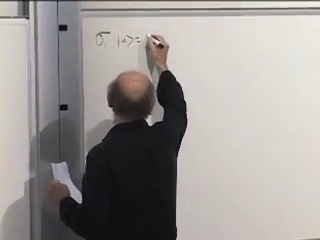
\includegraphics[width=0.62\linewidth]{lecture_05_figure_02.png}
\caption{비교 과정에서 사용하는 파울리 연산자의 전체 작용표.}
\lectureframe{00:03:15}
\end{figure}

두 상태 모두에서 어느 한쪽 스핀에도 선호되는 방향은 없다.
\begin{equation}
  \expect{\sigma_i}_{\psi_\pm}=0,
  \qquad
  \expect{\tau_i}_{\psi_\pm}=0,
  \qquad i=1,2,3.
  \label{eq:l05-local-zero}
\end{equation}
예를 들어, 요청된 플러스 상태의 명시적 계산은 다음과 같다.
\begin{align}
  \bra{\psi_+}\sigma_3\ket{\psi_+}
  &=
  \frac12
  \bigl(\bra{ud}+\bra{du}\bigr)
  \bigl(\ket{ud}-\ket{du}\bigr)\nonumber\\
  &=
  \frac12(1-1)=0.
  \label{eq:l05-sigma3-expectation}
\end{align}
\(\braket{ud}{du}=0\)이므로 교차항은 사라진다.

\begin{figure}[htbp]
\centering
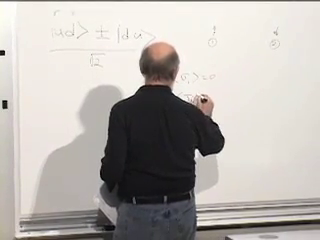
\includegraphics[width=0.78\linewidth]{lecture_05_figure_03.png}
\caption{플러스 상태의 기대값은 \(\sigma_3\)를 작용시키고 직교성을 이용해 계산한다.}
\lectureframe{00:07:00}
\end{figure}

\begin{classroomqa}
\lecturetimestamp{00:07:13}
\audiencequestion{기대값이 0이라는 것은 단일 스핀을 측정하면 값이 0으로 나온다는 뜻인가요?}
\lecturerresponse{아닙니다. 한 스핀 성분의 측정 결과는 \(+1\) 또는 \(-1\)뿐이며, \(\sigma_i\)에는 고윳값 0이 없습니다. 식~\eqref{eq:l05-local-zero}은 반복 측정 결과가 공정한 동전 던지기처럼 나온다는 뜻이지, 개별 측정 결과가 0이라는 뜻이 아닙니다.}
\end{classroomqa}

따라서 처음 생각해 볼 수 있는 진단 방법은 실패했다. 국소 평균으로는 상대 부호를 알 수 없으므로 두 입자쌍의 성질을 측정해야 한다.

\section{전체 스핀으로 단일항 상태를 판별하다}

입자쌍의 자기 모멘트는 벡터합으로 나타낸다.
\begin{equation}
  \boldsymbol{\Sigma}
  =
  \boldsymbol{\sigma}+\boldsymbol{\tau}.
\end{equation}
그 세 번째 성분은 두 기저 벡터 모두를 영벡터로 보낸다.
\begin{align}
  (\sigma_3+\tau_3)\ket{ud}
  &=(1-1)\ket{ud}=0,\nonumber\\
  (\sigma_3+\tau_3)\ket{du}
  &=(-1+1)\ket{du}=0.
\end{align}
따라서
\begin{equation}
  (\sigma_3+\tau_3)\ket{\psi_\pm}=0.
\end{equation}
어느 부호를 택하든 모든 시행에서 전체 세 번째 성분은 0이다.

첫 번째 성분은 두 상태를 구별한다. 식~\eqref{eq:l05-pauli-actions}에서,
\begin{align}
  (\sigma_1+\tau_1)\ket{ud}
  &=\ket{dd}+\ket{uu},\nonumber\\
  (\sigma_1+\tau_1)\ket{du}
  &=\ket{uu}+\ket{dd}.
\end{align}
따라서
\begin{align}
  (\sigma_1+\tau_1)\ket{\psi_+}
  &=
  \sqrt2\bigl(\ket{uu}+\ket{dd}\bigr),\nonumber\\
  (\sigma_1+\tau_1)\ket{\psi_-}
  &=0.
  \label{eq:l05-total-x}
\end{align}
플러스 상태에서 이 관측량의 기대값은 0일 수 있지만, 이 상태가 고윳값 0에 대응하는 고유상태인 것은 아니다.

\begin{classroomqa}
\lecturetimestamp{00:13:02}
\audiencequestion{전체 성분이 상태를 영벡터로 보내지 않을 때는 어떤 측정 결과가 가능한가요?}
\lecturerresponse{각 입자의 측정 결과는 \(+1\) 또는 \(-1\)이므로, 두 결과의 합은 \(2\), \(0\) 또는 \(-2\)일 수 있습니다. 기대값이 0이라고 해서 모든 시행에서 결과가 0인 것은 아닙니다.}
\end{classroomqa}

두 번째 성분을 확인하면 검증이 완성된다. 반대칭 조합에서는 \(i\)의 인자들이 상쇄된다.
\begin{equation}
  (\sigma_2+\tau_2)\ket{\psi_-}=0.
\end{equation}
따라서 세 성분 모두 마이너스 상태를 영벡터로 보낸다.
\begin{equation}
  \bigl(\boldsymbol{\sigma}+\boldsymbol{\tau}\bigr)
  \cdot\hat n\,\ket{\psi_-}=0
  \qquad\text{for every unit vector }\hat n.
  \label{eq:l05-singlet-any-axis}
\end{equation}

\begin{figure}[htbp]
\centering
\includegraphics[width=0.84\linewidth]{lecture_05_figure_06.png}
\caption{마이너스 상태의 전체 스핀이 0임을 보여 주는 성분별 상쇄.}
\lectureframe{00:16:30}
\end{figure}

반대칭 상태 \(\ket{\psi_-}\)는 \emph{단일항}이다. 이 상태는 회전 불변이다. 어느 축을 택해도 전체 스핀의 측정 결과는 0이다. 식~\eqref{eq:l05-two-signs}에 나오는 대칭 상태는 삼중항 부문에 속한다.

\begin{classroomqa}
\lecturetimestamp{00:19:06}
\audiencequestion{서로 반대인 스핀 결과는 평균적으로만 성립하나요?}
\lecturerresponse{단일항 상태에서는 모든 시행에서 성립합니다. 식~\eqref{eq:l05-singlet-any-axis}은 고유벡터 방정식이므로 두 입자에서 같은 성분을 측정하면 언제나 그 합이 고윳값 0인 결과를 얻습니다.}
\end{classroomqa}

\begin{classroomqa}
\lecturetimestamp{00:19:36}
\audiencequestion{다른 상태는 왜 삼중항이라고 부르나요?}
\lecturerresponse{그 이름은 전체 스핀 1 다중항에 속하는 세 상태에서 왔습니다. 유도는 나중으로 미루고, 여기서는 대칭 상태와 1차원 단일항 부문의 차이만 살펴보겠습니다.}
\end{classroomqa}

밥이 전자에서 임의의 성분을 측정하면, 앨리스가 자기 전자에서 같은 성분을 측정했을 때 어떤 결과를 얻을지 바로 알 수 있다. 앨리스의 결과는 반드시 그 반대다. 이것이 아인슈타인--포돌스키--로젠 상관관계다. 숨은 결과가 서로 반대인 동전 두 개도 있을 수 있지만, 미리 정해 둔 질문 하나에 대해서만 그렇다. 단일항 상태에서는 어떤 공간축을 선택하든 완벽한 반상관성이 성립한다.

\begin{classroomqa}
\lecturetimestamp{00:20:55}
\audiencequestion{얽힘을 처음 발견한 사람은 아인슈타인, 포돌스키, 로젠인가요?}
\lecturerresponse{아닙니다. 슈뢰딩거가 이 현상을 논의하고 얽힘이라는 용어를 도입했습니다. EPR 논증은 멀리 떨어진 입자 사이의 상관관계 문제를 특히 선명하게 드러냈습니다.}
\end{classroomqa}

\begin{classroomqa}
\lecturetimestamp{00:23:50}
\audiencequestion{즉각적인 상관관계는 인과율에 어긋나나요? 어느 관찰자가 먼저 측정하는지가 중요한가요?}
\lecturerresponse{전달할 수 있는 신호는 없습니다. 밥이 측정했는지와 관계없이, 어떤 관성계에서 보더라도 앨리스의 국소 측정 결과는 각각 절반의 확률로 나온다. 앨리스가 상관관계를 확인하려면 밥의 결과를 보통의 고전적 통신 채널로 전달받아야 하며, 그 신호는 빛보다 빠를 수 없다.}
\end{classroomqa}

\section{벨 부등식은 고전적인 계수 부등식이다}

벨의 결과가 무엇을 뜻하는지는 때로 분명하지 않게 느껴진다. 어떤 때는 양자역학의 가장 깊은 특징처럼 보이고, 다른 때는 형식론에서 필연적으로 따라 나오는 결과 중 하나처럼 보인다. 벨 자신도 파인먼도 이 두 관점을 모두 표현할 수 있었다. 하지만 부등식 자체는 기초적이다. 놀라운 점은 그것이 위반된다는 사실이다.

보통의 물체 집합을 생각해 보자. 각 물체는 세 성질 \(A\), \(B\), \(C\)을 가질 수도 있고 갖지 않을 수도 있다. \(N(A,\neg B)\)는 \(A\)은 가지지만 \(B\)은 갖지 않는 물체의 수를 나타내자. 고전적 집합 논리로부터 다음이 성립한다.
\begin{equation}
  N(A,\neg B)+N(B,\neg C)
  \geq
  N(A,\neg C).
  \label{eq:l05-bell-count}
\end{equation}
증명은 다음 집합 포함 관계에 따른다.
\begin{equation}
  A\cap C^{c}
  \subseteq
  (A\cap B^{c})\cup(B\cap C^{c}).
  \label{eq:l05-set-inclusion}
\end{equation}
실제로 \(A\cap C^c\)의 원소는 \(B\)에 속하거나 속하지 않는다. 첫 번째 경우에는 \(B\cap C^c\)에 속하고, 두 번째 경우에는 \(A\cap B^c\)에 속한다. 합집합의 원소 수를 세면 왼쪽 집합의 원소 수보다 많아질 수는 있어도 적어지지는 않는다.

\begin{figure}[htbp]
\centering
\includegraphics[width=0.78\linewidth]{lecture_05_figure_07.png}
\caption{칠판 위의 증명은 서로 겹치는 세 고전적 부분집합을 음이 아닌 영역들로 나눈다.}
\lectureframe{00:31:15}
\end{figure}

달리 말해, 세 집합 도형의 서로 겹치지 않는 영역에 음이 아닌 정수 \(N_i\)를 붙이자. 식~\eqref{eq:l05-bell-count}의 양변에는 \(A\cap C^c\)에 필요한 영역이 모두 포함되고, 왼쪽에는 음이 아닌 영역이 추가로 들어간다. 양자적인 내용은 전혀 개입하지 않는다. 이는 부분집합과 일반적인 논리적 선택지에 관한 정리다.

\section{집합 명제를 스핀 실험으로 옮기기}

많은 전자쌍을 서로 독립적으로 준비해 단일항 상태에 두고, 전자 1에 관해 다음 세 명제를 정의하자.
\begin{align}
  A&:\ \text{spin 1 is up at }0^\circ\text{, along the third axis},\nonumber\\
  B&:\ \text{spin 1 is up at }45^\circ\text{ in the }zx\text{-plane},\nonumber\\
  C&:\ \text{spin 1 is up at }90^\circ\text{, along the first axis}.
  \label{eq:l05-abc}
\end{align}

\begin{figure}[htbp]
\centering
\includegraphics[width=0.82\linewidth]{lecture_05_figure_08.png}
\caption{세 스핀 명제는 한 평면 안의 \(0^\circ\), \(45^\circ\), \(90^\circ\) 방향으로 정해져 있다.}
\lectureframe{00:39:00}
\end{figure}

단일항 상태에서는 전자 1에 관한 명제의 부정을 전자 2에 관한 긍정 명제로 바꿔 쓸 수 있다. 예를 들어,
\begin{align}
  \neg B
  &:\ \text{spin 1 is down at }45^\circ\nonumber\\
  &\Longleftrightarrow
  \text{spin 2 is up at }45^\circ.
\end{align}
마찬가지로 \(\neg C\)은 전자 2가 \(90^\circ\) 방향에서 위쪽이라는 명제가 된다.

\begin{classroomqa}
\lecturetimestamp{00:40:04}
\audiencequestion{\(\neg C\)는 전자 2가 \(90^\circ\) 방향에서 아래쪽임을 뜻하나요?}
\lecturerresponse{아닙니다. 먼저 \(C\)를 부정하면 전자 1는 \(90^\circ\) 방향에서 아래쪽입니다. 단일항 상태의 완벽한 반상관성에 따라 전자 2는 같은 축을 따라 위쪽이 됩니다. 이 두 번의 반전을 구분해야 합니다.}
\end{classroomqa}

계가 충분히 크면 계수와 확률의 차이는 준비된 쌍의 공통 개수뿐이다. 회전 불변성으로부터 다음도 성립한다.
\begin{equation}
  P(A,\neg B)=P(B,\neg C),
\end{equation}
두 번째 실험은 첫 번째 실험을 \(45^\circ\)만큼 회전한 것이기 때문이다. 따라서 벨의 고전적 부등식은 다음을 요구한다.
\begin{equation}
  2P(A,\neg B)\geq P(A,\neg C).
  \label{eq:l05-bell-probability}
\end{equation}
이제 이 확률들을 효율적으로 계산할 방법이 필요하다.

\section{명제를 투영 연산자로 나타내기}

보통의 3차원 벡터 공간에서 투영 연산자는 선택한 부분공간에 수직인 성분을 모두 제거한다. 1차원 투영 연산자는 벡터를 직선에 직교 투영하고, 2차원 투영 연산자는 평면에 직교 투영한다. \(P\)가 특정 부분공간으로의 투영 연산자라면,
\begin{equation}
  P\ket{\alpha}=\ket{\alpha_P}.
\end{equation}

\begin{figure}[htbp]
\centering
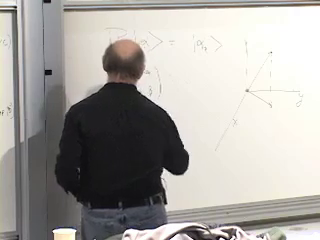
\includegraphics[width=0.76\linewidth]{lecture_05_figure_04.png}
\caption{기하학적 투영과 그 연산자 표기를 나란히 살펴본다.}
\lectureframe{00:49:53}
\end{figure}

\begin{figure}[htbp]
\centering
\begin{tikzpicture}[scale=1.05,>=Latex]
  \draw[->] (-0.25,0)--(4.0,0);
  \draw[thick] (-0.25,-0.25)--(3.55,2.6);
  \draw[->,very thick] (0,0)--(2.25,3.05)
    node[above] {\(\ket{\alpha}\)};
  \coordinate (P) at (2.72,1.98);
  \draw[dashed] (2.25,3.05)--(P);
  \draw[->,very thick] (0,0)--(P)
    node[right] {\(\ket{\alpha_P}\)};
  \node[below right] at (3.1,2.25) {projected subspace};
\end{tikzpicture}
\caption{투영 기하를 명확하게 다시 구성한 그림.}
\end{figure}

한 스핀의 힐베르트 공간에서 \(\sigma_3=+1\)이라는 명제는 \(\ket{u}\)가 생성하는 1차원 부분공간에 대응한다. 그 투영 연산자의 작용은 다음과 같다.
\begin{equation}
  P_{\sigma_3=+1}
  \begin{pmatrix}\alpha\\\beta\end{pmatrix}
  =
  \begin{pmatrix}\alpha\\0\end{pmatrix},
  \qquad
  P_{\sigma_3=-1}
  \begin{pmatrix}\alpha\\\beta\end{pmatrix}
  =
  \begin{pmatrix}0\\\beta\end{pmatrix}.
  \label{eq:l05-projector-actions}
\end{equation}

\begin{classroomqa}
\lecturetimestamp{00:49:55}
\audiencequestion{첫 번째 투영 연산자는 벡터가 수직축에서 얼마나 높은지 나타내나요?}
\lecturerresponse{아닙니다. 직교 성분인 \(\beta\)만 버립니다. 성분들은 힐베르트 공간의 진폭이지, 스핀의 보통 공간 좌표가 아닙니다.}
\end{classroomqa}

\begin{figure}[htbp]
\centering
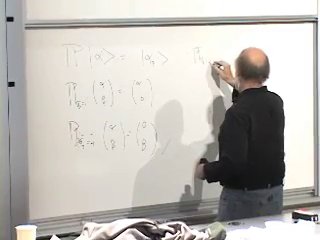
\includegraphics[width=0.78\linewidth]{lecture_05_figure_05.png}
\caption{투영 연산자를 먼저 일반적인 스피너에 작용시킨 다음 명시적인 행렬로 나타낸다.}
\lectureframe{00:51:40}
\end{figure}

행렬 형태는 다음과 같다.
\begin{equation}
  P_{\sigma_3=+1}
  =
  \begin{pmatrix}1&0\\0&0\end{pmatrix}
  =
  \frac{I+\sigma_3}{2}.
  \label{eq:l05-p3}
\end{equation}
같은 구성은 임의의 단위벡터 \(\hat n\) 방향에도 적용된다.
\begin{equation}
  P_{\boldsymbol{\sigma}\cdot\hat n=+1}
  =
  \frac{I+\boldsymbol{\sigma}\cdot\hat n}{2}.
  \label{eq:l05-pn}
\end{equation}

\begin{classroomqa}
\lecturetimestamp{00:53:09}
\audiencequestion{\(\sigma_1=+1\)에 대한 투영 연산자는 무엇인가요?}
\lecturerresponse{식~\eqref{eq:l05-p3}에서 \(\sigma_3\)를 \(\sigma_1\)로 바꾸면 됩니다. 즉, \(P_{\sigma_1=+1}=(I+\sigma_1)/2\)입니다.}
\end{classroomqa}

이제 보른 규칙을 명제의 형태로 유용하게 쓸 수 있다.
\begin{equation}
  P(\mathcal A\text{ is true in }\ket{\psi})
  =
  \bra{\psi}P_{\mathcal A}\ket{\psi}.
  \label{eq:l05-projector-born}
\end{equation}
정규화된 스피너 \(\ket{\psi}=(\alpha,\beta)^T\)에 대해 식~\eqref{eq:l05-projector-born}에서 \(P_{\sigma_3=+1}\)를 택하면 \(|\alpha|^2\)을 얻으며, 이는 예상한 결과다.

이 표현을 통해 고전적 명제와 양자 명제의 차이가 드러난다. 고전 논리에서 성질은 집합의 부분집합에 대응한다. 양자역학에서 성질은 힐베르트 공간의 부분공간, 또는 그에 대응하는 투영 연산자에 해당한다. 부분집합과 벡터 부분공간은 같은 격 연산을 따르지 않는다. 벨의 모순은 바로 그 차이에서 비롯된다.

\subsection{벨의 공동 투영 연산자}

\(A\wedge\neg B\)의 경우, 전자 1는 세 번째 축 방향으로 위쪽이어야 하고 전자 2는 다음 방향을 따라 위쪽이어야 한다.
\begin{equation}
  \hat n_{45}=\frac{\hat x+\hat z}{\sqrt2}.
\end{equation}
두 번째 스핀의 해당 성분은 다음과 같다.
\begin{equation}
  \boldsymbol{\tau}\cdot\hat n_{45}
  =
  \frac{\tau_1+\tau_3}{\sqrt2}.
\end{equation}
따라서 공동 투영 연산자는 다음과 같다.
\begin{equation}
  P_{A\wedge\neg B}
  =
  \frac{I+\sigma_3}{2}
  \frac{I+(\tau_1+\tau_3)/\sqrt2}{2}.
  \label{eq:l05-joint-projector}
\end{equation}

\begin{classroomqa}
\lecturetimestamp{00:59:18}
\audiencequestion{\(1/\sqrt2\)라는 계수가 \(45^\circ\) 스핀 성분에 들어가는 이유는 무엇인가요?}
\lecturerresponse{방향 벡터는 단위벡터여야 합니다. 첫 번째 축과 세 번째 축 방향의 성분이 모두 \(1/\sqrt2\)이므로, 이에 대응하는 관측량은 \((\tau_1+\tau_3)/\sqrt2\)입니다.}
\end{classroomqa}

\begin{classroomqa}
\lecturetimestamp{01:00:52}
\audiencequestion{식 전체 \(I+\boldsymbol{\tau}\cdot\hat n_{45}\)을 2로 나누나요?}
\lecturerresponse{네. 투영 연산자는 \(\bigl(I+\boldsymbol{\tau}\cdot\hat n_{45}\bigr)/2\)이며, 계수 \(1/2\)는 분자 전체에 곱해집니다.}
\end{classroomqa}

식~\eqref{eq:l05-joint-projector}의 두 인자는 서로 다른 텐서 인자에 작용하므로 서로 교환한다. 두 인자를 차례로 적용하면 먼저 전자 1가 아래쪽인 성분을 모두 제거하고, 남은 성분 가운데 전자 2가 \(\hat n_{45}\) 방향에서 아래쪽인 성분을 제거한다.

\section{양자수는 부등호의 방향을 뒤집는다}

다음을
\begin{equation}
  \ket{\psi_s}
  =
  \frac{\ket{ud}-\ket{du}}{\sqrt2}
\end{equation}
단일항 상태라 하자. 먼저 다음 식에서 시작한다.
\begin{equation}
  P(A,\neg B)
  =
  \bra{\psi_s}P_{A\wedge\neg B}\ket{\psi_s}.
\end{equation}
인자 \((I+\sigma_3)/2\)는 \(\ket{du}\)을 없애고 \(\ket{ud}/\sqrt2\)만 남긴다. 이어서 두 번째 인자를 적용하면
\begin{align}
  \frac{I+(\tau_1+\tau_3)/\sqrt2}{2}\ket{ud}
  &\notag\\[-0.3em]
  &=
  \frac12
  \left[
    \ket{ud}
    +\frac{\ket{uu}-\ket{ud}}{\sqrt2}
  \right]\nonumber\\
  &=
  \frac12
  \Biggl[
    \left(1-\frac1{\sqrt2}\right)\ket{ud}
  \nonumber\\
  &\qquad
    +\frac1{\sqrt2}\ket{uu}\Biggr].
  \label{eq:l05-projector-action}
\end{align}
\(\ket{uu}\)항은 단일항 브라와의 내적이 0이고, 남는 정규화 인자들을 계산하면 다음을 얻는다.
\begin{equation}
  P(A,\neg B)
  =
  \frac14\left(1-\frac1{\sqrt2}\right).
  \label{eq:l05-pab}
\end{equation}

\begin{figure}[htbp]
\centering
\includegraphics[width=0.88\linewidth]{lecture_05_figure_09.png}
\caption{투영 연산자 계산에서는 \(\ket{ud}\)와 겹치는 성분을 남기고 직교하는 \(\ket{uu}\) 성분을 제거한다.}
\lectureframe{01:08:20}
\end{figure}

회전 불변성에 따라 다음 두 방향에서도 같은 결과를 얻는다.
\begin{equation}
  P(B,\neg C)
  =
  \frac14\left(1-\frac1{\sqrt2}\right).
\end{equation}
\(A\wedge\neg C\)의 경우 두 번째 축이 첫 번째 공간축과 같으므로,
\begin{equation}
  P_{A\wedge\neg C}
  =
  \frac{I+\sigma_3}{2}\frac{I+\tau_1}{2}.
\end{equation}
첫 번째 인자는 다시 \(\ket{ud}/\sqrt2\)만 남긴다. \(\tau_1\) 항은 \(\ket{uu}\)를 만들며, 이는 단일항 브라와 직교한다. 반면 항등 연산자 항은 살아남는다. 따라서
\begin{equation}
  P(A,\neg C)=\frac14.
  \label{eq:l05-pac}
\end{equation}
세 결과를 합치면,
\begin{equation}
  \underbrace{
  P(A,\neg B)+P(B,\neg C)
  }_{\frac12(1-1/\sqrt2)\approx0.146}
  <
  \underbrace{
  P(A,\neg C)
  }_{\frac14=0.25}.
  \label{eq:l05-bell-violation}
\end{equation}

\begin{figure}[htbp]
\centering
\includegraphics[width=0.84\linewidth]{lecture_05_figure_10.png}
\caption{완성된 칠판 계산은 벨 부등식의 왼쪽 값이 더 작고 오른쪽 값이 더 큼을 보여 준다.}
\lectureframe{01:12:15}
\end{figure}

식~\eqref{eq:l05-bell-violation}은 식~\eqref{eq:l05-bell-probability}을 뒤집는다. 그렇다고 양자역학이 자기모순이라는 뜻은 아니다. 단일항 상관관계는 세 스핀 명제 모두가 먼 곳의 측정 선택과 무관하게 통상적인 집합론적 참·거짓 값을 가진다고 보는 국소적 고전 모형으로는 설명할 수 없다. 고전적 모형으로 이 상관관계를 재현하려면 벨 가정 가운데 적어도 하나를 포기해야 하며, 가장 두드러진 가정은 국소성이다.

\section{벨 실험이 검증하는 것}

양자역학은 이미 부등식 위반을 예측한다. 여기에 더해 실험에서는 한 검출기가 상대편 검출기에 자신이 만난 설정이나 결과를 알려 주는 고전적 우회 경로를 차단해야 한다. 두 측정 장치는 충분히 멀리 떨어져 있어야 하며, 측정 설정의 선택과 검출 시점은 빛의 속도로도 장치 사이를 오갈 수 없을 만큼 가까운 시간 간격 안에 있어야 한다. 아스페의 실험은 그러한 시간 조건과 분리를 실질적으로 납득할 수 있게 했다.

\begin{classroomqa}
\lecturetimestamp{01:13:15}
\audiencequestion{양자역학이 이미 답을 준다면 벨 실험은 무엇을 밝혔나요?}
\lecturerresponse{자연이 바로 이 상관관계 실험에서 양자역학의 예측을 따르는지 검증했고, 특히 두 측정 장치가 관련된 빛의 이동 시간 동안 서로 독립적으로 작동하도록 했습니다. 실험 제어와 시간 조정 자체도 상당한 성과였습니다.}
\end{classroomqa}

\begin{classroomqa}
\lecturetimestamp{01:18:19}
\audiencequestion{아인슈타인의 으스스한 원격 작용 논의에 벨은 무엇을 보탰나요?}
\lecturerresponse{벨은 정량적인 부등식을 제시했습니다. 철학적 불편함을 이야기하는 데 그치지 않고, 양자역학의 예측으로 국소적 고전 이론을 배제할 수 있는 실행 가능한 상관관계 실험을 찾아냈습니다. 벨은 이것이 필연적인 결과인지 심오한 발견인지에 대해 양가적인 태도를 보였고, 표준 양자역학에 점점 더 의문을 제기했습니다.}
\end{classroomqa}

입자들은 수 킬로미터 떨어져 있어도 하나의 공동 상태를 공유할 수 있지만, 이는 여전히 작은 계에서 하는 양자 실험이다. 환경과의 상호작용은 필요한 위상 관계를 쉽게 파괴한다. 공기 분자, 잡광자, 열적 교란이 입자쌍과 얽힐 수 있으므로, 실험은 차갑고 잘 격리된 환경에서 수행해야 한다.

\begin{classroomqa}
\lecturetimestamp{01:19:53}
\audiencequestion{공간적으로 넓게 퍼진 공동 상태라면 거시적 양자 물체라고 할 수 있나요?}
\lecturerresponse{서로 멀리 떨어진 작은 양자계라고 하는 편이 더 정확합니다. 두 계 사이의 거리는 클 수 있지만, 제어되지 않는 환경과의 상호작용이 유용한 결맞음을 파괴하므로 공동 파동함수를 보존하기는 점점 더 까다로워집니다. 보통의 볼링공 두 개로는 같은 실험을 할 수 없습니다.}
\end{classroomqa}

\begin{classroomqa}
\lecturetimestamp{01:21:23}
\audiencequestion{한 입자를 측정해 다른 입자의 상보적인 정보를 알아내면 불확정성 원리를 피할 수 있나요?}
\lecturerresponse{예를 들어 한 입자의 위치와 다른 입자의 운동량을 측정할 수는 있습니다. 이는 한 입자에서 서로 교환하지 않는 관측량을 동시에 측정하는 것이 아닙니다. 단일 계에 적용되는 불확정성 제약을 피한 것이 아닙니다.}
\end{classroomqa}

\section{곱이 언제 논리곱을 뜻할까?}

벨 계산에서는 두 투영 연산자를 곱했다. 이는 서로 양립 가능한 명제일 때만 논리곱을 나타낸다.

\begin{classroomqa}
\lecturetimestamp{01:22:39}
\audiencequestion{투영 연산자 두 개의 곱이 왜 논리적 ‘그리고’를 나타내나요?}
\lecturerresponse{두 투영 연산자가 교환하기 때문입니다. 하나는 전자 1에, 다른 하나는 전자 2에 작용하므로 순서가 중요하지 않고 두 성질을 함께 검사할 수 있습니다. 한 전자에서 \((I+\sigma_3)/2\)와 \((I+\sigma_1)/2\)는 교환하지 않습니다. 따라서 이 경우에는 두 축 방향으로 동시에 위쪽인 상태가 이런 의미에서 확정된 명제가 아닙니다.}
\end{classroomqa}

양자 명제와 보통의 부분집합이 다른 점이 여기서도 드러난다. 고전적 교집합은 언제나 존재한다. 양자에서 곱으로 나타내는 대응물은 관련 부분공간이 서로 양립할 때에만 의도한 논리적 의미를 갖는다.

이 논의는 측정 자체를 생각해 보게 한다. 측정 장치에는 지시자 상태가 있다. 위쪽 전자가 지시자를 한 방향으로 움직이고 아래쪽 전자가 다른 방향으로 움직인다면, 중첩 상태의 전자는 두 지시자 위치와 얽히게 된다. 따라서 측정은 계와 장치 사이의 얽힘으로 연구할 수 있다. 다만 여기서는 선형성만으로 증명할 수 있는 더 짧은 정리를 다루기 위해 그 문제는 뒤로 미룬다.

\begin{classroomqa}
\lecturetimestamp{01:25:09}
\audiencequestion{파동함수 붕괴를 한 번의 측정이 공동 상태를 제약하는 과정으로 이해할 수 있나요?}
\lecturerresponse{그 질문은 측정 과정에 관한 것입니다. 장치와 측정 대상 계는 얽히게 됩니다. 한 스핀 값은 한 지시자 위치와, 다른 스핀 값은 또 다른 위치와 상관됩니다. 측정에 관한 자세한 논의는 뒤로 미루겠습니다.}
\end{classroomqa}

\section{선형성은 보편 복제기를 허용하지 않는다}

시간 변화에 관해서는 한 가지 사실만 필요하다. 물리적 과정이 다음과 같이 변환한다면,
\begin{equation}
  \ket{a}\longrightarrow\ket{a'},
  \qquad
  \ket{b}\longrightarrow\ket{b'},
\end{equation}
선형성에 따라 다음 변환이 성립해야 한다.
\begin{equation}
  \alpha\ket{a}+\beta\ket{b}
  \longrightarrow
  \alpha\ket{a'}+\beta\ket{b'}.
  \label{eq:l05-linearity}
\end{equation}

보통의 복사기는 제어 가능한 작은 오차로 고전 정보를 복제할 수 있다. 양자 복제에 대한 요구는 더 강하다. 하나의 고정된 장치가 어떤 상태를 입력받더라도 그 상태의 모든 진폭을 복제해야 한다. 그래서 복제 금지를 양자 복사 금지 원리라고도 부른다.

입력 포트 하나와 출력 포트 두 개가 있는 기계를 생각해 보자. 이 기계가 세 번째 축의 기저 상태들을 복제한다면, 다음과 같이 작동해야 한다.
\begin{equation}
  \ket{u}\longrightarrow\ket{uu},
  \qquad
  \ket{d}\longrightarrow\ket{dd}.
  \label{eq:l05-clone-basis}
\end{equation}
기계가 출력에 에너지, 질량 또는 전하를 공급할 수는 있으므로, 보존 법칙에 따른 계산이 장애물인 것은 아니다. 모순은 변환이 상태에 의존하는 방식에서 생긴다.

\begin{figure}[H]
\centering
\includegraphics[width=0.86\linewidth]{lecture_05_figure_11.png}
\caption{입력 하나와 출력 둘을 가진 가상 기계가 두 기저 상태 모두를 복제하도록 요구받는다.}
\lectureframe{01:33:45}
\end{figure}

이제 오른쪽을 향하는 스핀을 입력하자.
\begin{equation}
  \ket{r}
  =
  \frac{\ket{u}+\ket{d}}{\sqrt2}.
  \label{eq:l05-right-state}
\end{equation}
식~\eqref{eq:l05-linearity}과 \eqref{eq:l05-clone-basis}에 따라 출력은 다음과 같아야 한다.
\begin{equation}
  \ket{r}
  \longrightarrow
  \frac{\ket{uu}+\ket{dd}}{\sqrt2}.
  \label{eq:l05-linear-output}
\end{equation}
정확한 복제라면 독립적인 복사본 두 개를 만들어야 한다.
\begin{align}
  \ket{rr}
  &=
  \ket{r}\otimes\ket{r}\nonumber\\
  &=
  \frac12
  \left(
    \ket{uu}+\ket{ud}+\ket{du}+\ket{dd}
  \right).
  \label{eq:l05-cloned-output}
\end{align}
식~\eqref{eq:l05-cloned-output}에는 식~\eqref{eq:l05-linear-output}에 없는 혼합항이 들어 있다. 두 출력은 서로 다르다.

\begin{figure}[H]
\centering
\includegraphics[width=0.72\linewidth]{lecture_05_figure_12.png}
\caption{선형성으로는 평행한 스핀 항만 나오지만, 오른쪽을 향하는 스핀을 두 개 복제하면 혼합항 두 개도 나온다.}
\lectureframe{01:35:20}
\end{figure}

\begin{theorem}[No-cloning]
어떤 단일 물리적 기계도 모든 미지의 양자 상태를 정확히 복제할 수 없다.
\end{theorem}

\begin{proof}
한 기계가 식~\eqref{eq:l05-clone-basis}처럼 직교 기저 상태를 복제한다고 가정하자. 그러면 선형성에 따라 중첩 상태의 출력은 식~\eqref{eq:l05-linear-output}으로 정해진다. 같은 입력을 정확히 복제하려면 식~\eqref{eq:l05-cloned-output}가 요구된다. 두 상태 벡터가 다르므로, 가정한 보편 기계는 존재할 수 없다.
\end{proof}

이유는 구조에 있다. \(\ket{\psi}\)을 \(\ket{\psi}\otimes\ket{\psi}\)로 변환하는 것은 진폭에 대해 이차적이지만, 완전한 양자 상태의 허용된 시간 변화는 모두 선형이다.

\begin{classroomqa}
\lecturetimestamp{01:35:49}
\audiencequestion{이 증명은 출력 두 개가 서로 독립적이라고 가정하나요?}
\lecturerresponse{그렇습니다. 복제본 두 개라면 각각 독립적으로 사용할 수 있어야 하기 때문입니다. 독립적인 계를 결합할 때는 텐서곱을 사용하므로, 오른쪽을 향하는 스핀 두 개는 \(\ket{r}\otimes\ket{r}\)입니다. 서로 독립적으로 쓸 수 없는 상관된 출력은 복제본 두 개가 아닙니다.}
\end{classroomqa}

\begin{classroomqa}
\lecturetimestamp{01:37:20}
\audiencequestion{레이저는 유도 방출로 광자의 상태를 복사하는 것처럼 보입니다. 이 논증은 어디서 적용되지 않나요?}
\lecturerresponse{원자와 전자기 모드도 과정에 참여합니다. 보편 복제의 관점에서 보면 이들의 상태도 출력에 기여하고 잡음으로 나타납니다. 근사 복제는 가능하지만, 완벽하고 상태에 무관한 복제는 불가능합니다.}
\end{classroomqa}

\begin{classroomqa}
\lecturetimestamp{01:40:24}
\audiencequestion{양자 정보는 복제할 수 없어도 전송할 수 있나요?}
\lecturerresponse{네. 전송은 다른 연산입니다. 원래 상태를 가진 계가 그 상태를 계속 유지할 필요는 없습니다. 복제 금지가 금하는 것은 완벽한 복사본 두 개를 남기는 일이지, 한 운반체에서 다른 운반체로 상태를 옮기는 일이 아닙니다.}
\end{classroomqa}

\begin{classroomqa}
\lecturetimestamp{01:41:03}
\audiencequestion{입력 상태는 미지의 상태여야 하나요?}
\lecturerresponse{상태를 미리 알고 있다면 그 상태의 계를 더 준비하거나, 선택한 직교 기저에 맞춘 장치를 만들 수 있습니다. 불가능한 것은 임의의 입력을 받아 어떤 상태가 들어왔는지 미리 알지 못한 채 복제하는 기계입니다.}
\end{classroomqa}

\begin{classroomqa}
\lecturetimestamp{01:42:35}
\audiencequestion{오른쪽 상태를 나타내는 두 식 가운데 실제 기계의 출력은 어느 것인가요?}
\lecturerresponse{선형성은 식~\eqref{eq:l05-linear-output}을 강제하고, 복제는 식~\eqref{eq:l05-cloned-output}을 요구합니다. 둘의 불일치가 바로 모순입니다.}
\end{classroomqa}

\begin{classroomqa}
\lecturetimestamp{01:43:40}
\audiencequestion{얽힌 두 입자 상태에 담긴 추가 정보를 정량화할 수 있나요?}
\lecturerresponse{한 스핀의 순수 상태에는 물리적인 실수 매개변수가 두 개 있습니다. 서로 따로 준비한 두 스핀에는 네 개가 있지만, 4차원 두 스핀 힐베르트 공간의 일반적인 순수 상태에는 정규화와 전체 위상을 제외하고도 여섯 개가 있습니다. 추가된 상태에는 얽힌 상태가 포함되며, 얽힘의 정도는 얽힘 엔트로피로 정량화할 수 있습니다.}
\end{classroomqa}

\enlargethispage{4\baselineskip}식~\eqref{eq:l05-two-signs}의 부호는 이제 세 가지 역할을 했다. 유일한 전체 스핀 0 상태를 선택했고, 고전적 집합 부등식을 위반하는 상관관계를 만들어 냈으며, 선형 양자 시간 변화와 두 복사본을 만드는 비선형 작용의 차이를 드러냈다. 이 결과들은 모두 공동 상태를 미리 정해진 국소 성질의 목록이 아니라 전체 텐서곱 공간의 벡터로 다룬 데서 나온다.

\graphicspath{{../../../generated_course_notes/supplementary/quantum_entanglement/2006_fall_part_1/chapters/lecture_06/}{../../../generated_course_notes/supplementary/quantum_entanglement/2006_fall_part_1/figures/}{../../../generated_course_notes/supplementary/quantum_entanglement/2006_fall_part_1/assets/}}
\chapter{부분공간, 사영 연산자, 그리고 얽힘으로서의 측정}

벨의 정리는 두 가지 질문을 남겼다. 얽힌 쌍의 한쪽이 교란되거나 흡수되거나 측정되면 얽힘은 어떻게 되는가? 그리고 정확히 무엇이 평범한 상호작용을 측정으로 바꾸는가? 답에 이르는 길은 기초 선형대수학을 거친다. 물리적 성질은 부분공간이고, 확률은 사영 연산자의 기댓값이며, 측정 장치는 대상과 얽히는 또 하나의 양자계다.

\section{도입: 얽힘, 국소성, 측정}

싱글렛이 멀리 떨어진 두 부분으로 나뉘고 그중 한쪽을 측정했다고 하자. 양자장론은 두 부분 사이에 가상 교환이 있었다고 기술해야 하는가? 먼 쪽에서는 검출 가능한 일이 일어나지 않고, 그곳에 보낼 수 있는 메시지도 전달되지 않는다. 자기장을 이용해 한쪽 스핀을 국소적으로 회전시켜 공동 상태의 구체적인 형태를 바꿀 수는 있지만, 그 국소 연산을 해도 얽힘의 양은 그대로다. 얽힘을 정량화하는 방법은 뒤에서 다룬다. 지금 중요한 점은 더 이상 상호작용하지 않는 두 계가 한쪽에만 국한된 연산만으로 공유 얽힘을 바꿀 수 없다는 것이다.

\begin{classroomqa}\lecturetimestamp{00:00:22}\audiencequestion{시공간적으로 분리된 싱글렛의 한쪽을 측정하려면 다른 쪽과 가상 교환이 있어야 하는가?}\lecturerresponse{다른 쪽에서는 검출 가능한 교환이 일어나지 않는다. 국소 연산으로 한 인자를 회전시켜 공동 상태를 표현하는 형태를 바꿀 수는 있지만, 그 연산만으로는 메시지를 보내거나 두 부분 사이에 공유된 얽힘을 바꿀 수 없다.}\end{classroomqa}

이 때문에 무엇을 얽힘의 상대 계로 볼지 더 폭넓게 생각해야 한다. 얽힌 쌍의 한쪽이 블랙홀에 빠지더라도 다른 쪽과의 얽힘이 사라지는 것은 아니다. 그 입자는 블랙홀의 자유도와 얽히고, 블랙홀이 증발한 뒤에는 방출된 복사와 얽힌다. 이와 같은 생각을 적용하는 데 블랙홀은 필요하지 않다. 얽힌 쌍의 한쪽을 욕조에 빠뜨려 물과 격렬하게 섞이게 해 보자. 다체 상태 속에서 그 입자의 개별 정체성은 사라질 수 있지만, 멀리 있는 입자는 여전히 욕조 전체와 얽혀 있고, 결국 빠져나가는 수증기와도 얽힌다.

이것은 얽힘이 지속된다는 이야기만은 아니다. 가역성에 관한 이야기이기도 하다. 상호작용으로 얽힘을 만들 수 있다면, 원칙적으로 상호작용으로 얽힘을 되돌릴 수도 있다. 얽힘을 풀 수는 있지만, 계들이 다시 접촉해 상호작용해야만 가능하다. 한 방향으로 일어날 수 있는 일은 반대 방향으로도 일어날 수 있다.

\begin{classroomqa}\lecturetimestamp{00:04:45}\audiencequestion{얽힌 쌍의 두 스핀을 모두 측정하면 전자들은 계속 얽혀 있는가? 측정 한 번만으로 이미 얽힘이 풀릴 수도 있는가?}\lecturerresponse{측정으로 둘 사이의 얽힘을 없앨 수 있으며, 측정 한 번이면 충분할 수도 있다. 단순히 파동 묶음의 붕괴라고 단언하는 대신 그 말이 무엇을 뜻하는지 알려면, 관측을 계와 기록 장치 사이의 상호작용으로 기술해야 한다.}\end{classroomqa}

이 질문이 우리가 다룰 과제를 정한다. 관측, 파동 묶음의 붕괴, 얽힘을 연결하는 것이다. 하지만 거기에 앞서, 필요한 만큼의 기초적인 도구만으로 부분공간과 사영 연산자를 더 명료하게 설명할 필요가 있다.

\section{차원, 선형 종속성, 정규직교 기저}

그러므로 우선 브라, 켓, 내적을 갖춘 유한 차원 벡터 공간을 다룬다. 서스킨드는 가능한 한 기초적인 방식으로 시작한다. 열벡터의 성분을 세어 차원을 정의하지 않는다. 차원을 추상적으로 정의한다. 벡터 공간의 차원이란 그 안에서 찾을 수 있는 선형 독립 벡터의 최대 개수다.

따라서 벡터들의 모임 \(\{|v_i\rangle\}\)은 다음 관계에서 \begin{equation}
\sum_i c_i |v_i\rangle = 0
\end{equation} 모든 계수 \(c_i\)가 영이 되는 경우 선형 독립이다. 달리 말해, 어느 벡터도 나머지 벡터들의 선형 결합으로 나타낼 수 없다.

여기서 직교성과 선형 독립성은 서로 다르다는 점이 중요하다. 삼차원 공간에는 서로 전혀 직교하지 않으면서도 선형 독립인 벡터 세 개가 있을 수 있다. 중요한 것은 그중 하나를 나머지 두 벡터로 만들 수 있는지 여부다. 반면 이차원 평면에서는 그 평면 안의 세 번째 벡터가 앞의 두 벡터에 선형 종속일 수밖에 없다.

\begin{figure}[htbp]\centering
\includegraphics[width=0.56\textwidth]{lecture_06_figure_02.png}\caption{칠판에 그린 세 벡터. 강의에서는 이 그림으로 직교성과 선형 독립성을 구분한 뒤, 평면에서 세 번째 벡터가 앞의 두 벡터에 종속됨을 강조한다.}\lectureframe{00:09:35}\end{figure}

\begin{figure}[htbp]\centering
\begin{tikzpicture}[scale=1.2]
\draw[->] (0,0) -- (2.3,0);
\draw[->] (0,0) -- (2.0,2.0);
\draw[->] (0.35,0.95) -- (1.05,1.45);
\fill (0,0) circle (1.2pt);
\end{tikzpicture}\caption{칠판 그림을 간결하게 재구성한 것. 이 장면만으로는 구체적인 계수 관계를 정할 수 없다. 기하학적 요점은 이차원 평면의 세 번째 벡터는 선형 독립일 수 없다는 것이다.}\end{figure}

그림의 요점이 바로 이것이다. 공간의 차원이 이라면 선형 독립 벡터의 최대 개수는 둘이다. 공간의 차원이 삼이라면 최대 개수는 셋이다. 더 일반적으로 공간의 차원이 \(d\)이면, 내적이 주어졌을 때 그 공간을 생성하는 서로 직교하는 단위 벡터 \(d\)개를 찾을 수 있다. 이것들이 기저 벡터다. 서스킨드는 여기서 그 정리를 증명하지 않겠다고 분명히 말한다. 그가 강조하려는 결론은 이것이다. 그러한 기저가 있으면 공간의 모든 벡터를 그 기저 벡터들의 선형 결합으로 전개할 수 있다.

\begin{classroomqa}\lecturetimestamp{00:10:58}\audiencequestion{공간적 자유도의 개수는 상태 공간의 차원과 같은가?}\lecturerresponse{아니다. 방 안에서 움직이는 입자는 공간 좌표가 세 개지만 서로 직교하는 양자 상태는 엄청나게 많다. 배치 공간의 차원과 힐베르트 공간의 차원은 서로 다른 개념이다. 유한 차원 예제는 논리를 명료하게 보여 주기 위해서만 사용한다.}\end{classroomqa}

\section{기저 전개, 다이애드, 항등 연산자의 분해}

이제 \(\{|n\rangle\}\)을 정규직교 기저로 잡자. 여기서 \(n=1,\dots,d\)이다. 이 대목의 칠판 설명은 특히 명료하고 간결하다.

\begin{figure}[htbp]\centering
\includegraphics[width=0.62\textwidth]{lecture_06_figure_03.png}\caption{정규직교 기저와 임의의 상태의 전개.}\lectureframe{00:14:15}\end{figure}

다음과 같이 쓴다. \begin{align}
\langle m|n\rangle &= \delta_{mn}, \\
|\psi\rangle &= \sum_n a_n |n\rangle.
\end{align} 여기서 \(\delta_{mn}\)는 크로네커 델타다. \(m=n\)일 때는 \(1\)이고, 그렇지 않을 때는 \(0\)이다.

\paragraph{유도}계수는 기저에 사영해 구한다. 왼쪽에서 \(\langle m|\)를 곱하면 \begin{align}
\langle m|\psi\rangle
  &= \sum_n a_n \langle m|n\rangle \\
  &= \sum_n a_n \delta_{mn} \\
  &= a_m.
\end{align}가 된다. 따라서 계수는 간단히 \begin{equation}
a_m = \langle m|\psi\rangle.
\end{equation}와 같다. 계수는 보통의 복소수이므로 켓의 어느 쪽에 놓아도 값은 변하지 않는다.

이 계수를 전개식에 다시 대입하면 \begin{equation}
|\psi\rangle = \sum_n |n\rangle \langle n|\psi\rangle.
\end{equation}을 얻는다. 여기서 \(|n\rangle\langle n|\), 더 일반적으로 \(|a\rangle\langle b|\)를 연산자로 해석해야 한다는 생각이 나온다. 바로 이것이 다음 단계다. 다이애드는 다음과 같이 작용한다. \begin{equation}
\bigl(|a\rangle\langle b|\bigr)|\psi\rangle = \langle b|\psi\rangle\,|a\rangle.
\end{equation} 브라는 복소수를 뽑아내고, 켓은 그 결과에 해당하는 방향을 제공한다. 이는 벡터에서 연산자로 나아가는 서스킨드의 간단한 방법이다.

앞의 전개식을 연산자 관점에서 보자. \begin{equation}
|\psi\rangle = \left(\sum_n |n\rangle\langle n|\right)|\psi\rangle
\end{equation}가 모든 \(|\psi\rangle\)에 대해 성립하므로 괄호 안의 연산자는 항등 연산자여야 한다. \begin{equation}
\sum_n |n\rangle\langle n| = I.
\end{equation} 이것이 항등 연산자의 분해다.

\begin{figure}[htbp]\centering
\includegraphics[width=0.60\textwidth]{lecture_06_figure_07.png}\caption{칠판에 완성된 항등 연산자 분해.}\lectureframe{00:18:30}\end{figure}

\begin{classroomqa}\lecturetimestamp{00:18:39}\audiencequestion{항등 연산자 분해에 나오는 벡터들은 기저여야 하는가?}\lecturerresponse{그렇다. 유도 과정은 정규화와 상호 직교성을 모두 사용하며, 합은 완비 기저 전체에 대해 취해야 한다. 임의의 벡터 모임으로는 항등 연산자를 분해할 수 없다.}\end{classroomqa}

항등 연산자 자체가 공간 전체로의 사영 연산자다. 모든 벡터는 \(I\)의 고유벡터이고, 모든 고윳값은 \(+1\)이다.

\begin{classroomqa}\lecturetimestamp{00:19:14}\audiencequestion{항등 연산자의 분해는 모든 벡터의 고윳값이 일이라고 말하는가?}\lecturerresponse{그렇다. 항등 연산자의 경우에는 모든 벡터가 그 고유벡터이고 모든 상태에 대해 \(I|\psi\rangle=|\psi\rangle\)가 성립한다는 점에서 특별하다.}\end{classroomqa}

\section{부분공간으로서의 물리량과 사영 연산자}

이 도구들을 갖춘 뒤, 강의는 핵심 개념을 바로잡는다. \(k=\lambda\)와 같은 물리량은 일반적으로 벡터 하나를 뜻하지 않는다. 하나의 부분공간 전체를 뜻한다.

\(k\)를 에르미트 관측량이라 하고, \begin{equation}
k|A\rangle = \lambda |A\rangle, \qquad
k|B\rangle = \lambda |B\rangle,
\end{equation}라고 하자. 여기서 \(|A\rangle\)와 \(|B\rangle\)는 선형 독립이다. 그러면 임의의 선형 결합도 같은 고윳값을 갖는다. \begin{align}
k\bigl(\alpha|A\rangle+\beta|B\rangle\bigr)
  &= \alpha k|A\rangle + \beta k|B\rangle \\
  &= \alpha \lambda |A\rangle + \beta \lambda |B\rangle \\
  &= \lambda\bigl(\alpha|A\rangle+\beta|B\rangle\bigr).
\end{align} 그러므로 \(\lambda\)에 해당하는 고유공간은 덧셈과 스칼라 곱에 대해 닫혀 있다. 즉 벡터 부분공간이다.

강의에서 처음 드는 구체적인 예는 두 스핀 계다. 상태 \begin{equation}
|ud\rangle,\qquad |uu\rangle
\end{equation}는 두 번째 스핀의 값은 서로 다르지만 첫 번째 스핀의 값은 같다. 두 상태 모두 첫 번째 스핀이 위쪽이다. 따라서 두 상태는 첫 번째 스핀에서 \(\sigma_3=+1\)인 부분공간을 생성한다.

\begin{figure}[htbp]\centering
\includegraphics[width=0.46\textwidth]{lecture_06_figure_04.png}\caption{첫 번째 스핀이 위쪽인 두 스핀 상태.}\lectureframe{00:23:27}\end{figure}

기억해야 할 요점은 이것이다. 물리량이 반드시 상태 하나에 대응하는 것은 아니다. 같은 고윳값을 갖는 상태들의 집합 전체에 대응한다.

칠판에서 잠시 나타나는 표기상의 혼동을 피하기 위해, 특정 고유벡터에는 대문자 \(A,B,\dots\)를 쓰고, 고유부분공간의 정규직교 기저를 순회하는 합의 첨자에는 소문자 \(a,b,\dots\)를 쓰겠다. \(\{|a\rangle\}\)가 부분공간 \(k=\lambda\)의 기저라면, 그 부분공간으로의 사영 연산자는 다음과 같다. \begin{equation}
\Pi_{k=\lambda}=\sum_a |a\rangle\langle a|.
\end{equation} 이것은 부분공간에만 제한한 항등 연산자다. \(|\psi\rangle\)가 이미 그 부분공간에 있으면 사영 연산자는 이를 그대로 돌려준다. \(|\psi\rangle\)가 부분공간 밖에 걸쳐 있으면 직교하는 나머지 성분을 버리고 내부 성분만 남긴다.

\section{확률 공리, 양립 가능한 물리량, 그리고 벨 정리 복습}

물리량을 부분공간으로 다시 이해하고 나면 확률 공리는 가장 간결한 형태를 취한다. \(|\psi\rangle\)가 정규화되어 있을 때, 그 상태가 물리량 \(k=\lambda\)을 갖는 확률은 다음과 같다. \begin{equation}
P(k=\lambda)=\langle\psi|\Pi_{k=\lambda}|\psi\rangle.
\end{equation}

\begin{figure}[htbp]\centering
\includegraphics[width=0.58\textwidth]{lecture_06_figure_05.png}\caption{\(k=\lambda\)의 고유부분공간으로의 사영 연산자. 칠판의 표기는 다음 단계를 이미 예고한다. 사영 연산자를 \(\langle\psi|\)와 \(|\psi\rangle\) 사이에 끼워 넣는다.}\lectureframe{00:31:09}\end{figure}

사영 연산자를 다이애드 형태로 대입하면 \begin{align}
P(k=\lambda)
  &= \left\langle \psi \left| \sum_a |a\rangle\langle a| \right| \psi \right\rangle \\
  &= \sum_a \langle\psi|a\rangle\langle a|\psi\rangle \\
  &= \sum_a |\langle a|\psi\rangle|^2.
\end{align}을 얻는다. 이는 강의에서 설명한 그대로다. 해당 물리량에 대한 총확률은 그 물리량이 나타날 수 있는 서로 직교하는 모든 방식의 확률을 더한 것이다.

두 스핀 계에서 첫 번째 스핀이 위쪽인 상태와 관련된 부분공간은 \(|uu\rangle\)와 \(|ud\rangle\)가 생성하므로 \begin{equation}
\Pi_{\sigma_3=+1}=|uu\rangle\langle uu|+|ud\rangle\langle ud|.
\end{equation}이다. 강의에서는 두 번째 스핀에 작용하는 항등 연산자를 생략해 \begin{equation}
\Pi_{\sigma_3=+1}=\frac{1+\sigma_3}{2},
\end{equation}라고 줄여 쓰기도 한다.

\begin{classroomqa}\lecturetimestamp{00:33:04}\audiencequestion{관측량, 물리량, 사영 연산자의 차이는 무엇인가?}\lecturerresponse{관측량은 에르미트 연산자 \(k\)다. 물리량 \(k=\lambda\)는 그 고유부분공간으로 나타내며, \(k\)를 측정하면 반드시 \(\lambda\)가 나온다는 뜻이다. 사영 연산자 \(\Pi_{k=\lambda}\)는 그 부분공간을 분리해 내며, 그 기댓값은 해당 물리량이 나타날 확률을 준다.}\end{classroomqa}

\begin{classroomqa}\lecturetimestamp{00:34:07}\audiencequestion{축퇴 고유벡터 \(A\)와 \(B\)는 이미 서로 직교해야 하는가? 그리고 이 벡터들은 공간 전체의 기저인가?}\lecturerresponse{원래의 고유벡터들은 서로 직교할 필요가 없지만, 그 고유부분공간 안에서는 언제나 정규직교 기저를 선택할 수 있다. 그 기저는 해당 부분공간의 기저일 뿐이다. 전체 공간을 생성하려면 추가로 직교하는 방향들이 필요하다. 부분공간의 각 기저 벡터에 사영한 뒤 그 결과를 더하면 부분공간으로의 사영이 된다.}\end{classroomqa}

\begin{classroomqa}\lecturetimestamp{00:35:33}\audiencequestion{\(a\)라는 기호는 \(k|A\rangle=\lambda|A\rangle\)에서 쓰인 \(a\)와 사영 연산자에서 합을 취하는 첨자와 같은 뜻인가?}\lecturerresponse{아니다. 앞의 기호는 특정 고유벡터를 나타내지만, 합의 아래에 있는 첨자는 고유부분공간의 정규직교 기저에 속하는 모든 벡터를 순회한다. 표기를 구분하면 특정한 표지를 합의 더미 첨자로 오해하지 않게 된다.}\end{classroomqa}

\begin{classroomqa}\lecturetimestamp{00:37:15}\audiencequestion{사영 연산자 식에 나오는 내적은 확률인가, 확률 진폭인가?}\lecturerresponse{각각의 \(\langle a|\psi\rangle\)는 진폭이다. 여기에 복소켤레를 곱하면 확률이 되고, \(k=\lambda\)을 실현하는 서로 직교하는 여러 방식의 확률을 합하면 해당 물리량의 총확률이 된다.}\end{classroomqa}

이어서 강의는 물리량들을 결합하는 방법을 묻는다. 서로 양립하고 사영 연산자 \(P_k\)와 \(P_\ell\)로 나타내는 두 물리량이 있다고 하자. 강의의 표현을 따르면 AND 명제는 곱으로 나타낸다. \begin{equation}
\Pi_{k=\lambda\,\wedge\,\ell=\mu}=P_kP_\ell=P_\ell P_k.
\end{equation} 논리는 간단하다. \(P_k|\psi\rangle\)는 \(k=\lambda\) 부분공간에 속한다. 연산자들이 서로 가환하므로 \(P_\ell P_k|\psi\rangle=P_kP_\ell|\psi\rangle\)이고, 따라서 같은 벡터는 \(\ell=\mu\) 부분공간에도 속한다. 그러므로 두 연산자의 곱은 두 물리량이 동시에 성립하는 부분공간으로 사영한다. 이에 해당하는 확률은 \begin{equation}
P(k=\lambda,\ell=\mu)=\langle\psi|P_kP_\ell|\psi\rangle.
\end{equation}이다.

이 논증의 첫 단계는 따로 살펴볼 만하다. 임의의 상태에 대해 \begin{equation}
k\bigl(P_k|\psi\rangle\bigr)=\lambda P_k|\psi\rangle,
\end{equation}이므로 \(P_k|\psi\rangle\)는 \(k=\lambda\) 고유부분공간에 속한다. \(P_k\)와 \(P_\ell\)가 가환하면 곱을 어느 사영 연산자를 왼쪽에 두든 같은 형태로 쓸 수 있다. 따라서 그 결과는 두 부분공간 모두에 속한다.

\begin{figure}[htbp]\centering
\includegraphics[width=0.44\textwidth]{lecture_06_figure_06.png}\caption{고유부분공간에 속하는 벡터로서의 사영된 상태.}\lectureframe{00:41:57}\end{figure}

\begin{figure}[htbp]\centering
\begin{tikzpicture}[scale=1.1]
\draw (-2,0) -- (2,0);
\draw[->,thick] (0,0) -- (1.3,1.8) node[right] {$|\psi\rangle$};
\draw[dashed] (1.3,1.8) -- (1.3,0);
\draw[->,thick] (0,0) -- (1.3,0) node[below] {$P_k|\psi\rangle$};
\node at (0,-0.35) {$k=\lambda$ subspace};
\end{tikzpicture}\caption{\(k=\lambda\) 고유부분공간으로 임의의 벡터를 사영하는 모습.}\end{figure}

\begin{figure}[htbp]\centering
\begin{tikzpicture}[scale=1.0]
\draw (0,0) ellipse (2.1 and 1.2);
\draw (1.7,0) ellipse (2.1 and 1.2);
\node at (-0.7,0.95) {$k=\lambda$};
\node at (2.4,0.95) {$\ell=\mu$};
\node at (0.85,0) {AND};
\end{tikzpicture}\caption{가환 사영 연산자의 AND 명제 뒤에 있는 교차 부분공간 그림의 재구성.}\end{figure}

\begin{figure}[htbp]\centering
\includegraphics[width=0.66\textwidth]{lecture_06_figure_08.png}\caption{가환 사영 연산자가 동시 고유부분공간을 선택한다는 칠판 논증.}\lectureframe{00:45:20}\end{figure}

\begin{classroomqa}\lecturetimestamp{00:44:42}\audiencequestion{두 물리량이 동시에 성립하는 부분공간은 고전 논리에서의 교집합과 같은가?}\lecturerresponse{그렇다. 가환 사영 연산자에서 \(P_kP_\ell\)는 두 고유부분공간의 교집합으로 사영한다. 그 교집합이 영벡터만 포함한다면 두 물리량을 모두 갖는 영이 아닌 상태는 없다.}\end{classroomqa}

완전성을 위해, 양립 가능한 OR 부분공간으로의 사영 연산자는 다음과 같다. \begin{equation}
P_{k\lor\ell}=P_k+P_\ell-P_kP_\ell .
\end{equation} 두 대안이 서로 배타적이면 \(P_kP_\ell=0\)이므로 식은 합 \(P_k+P_\ell\)으로 단순해진다. 두 부분공간이 겹칠 때는 교집합을 두 번 세지 않도록 이 뺄셈이 반드시 필요하다.

이어 양립 가능성은 물리적 예와 연결된다. 두 스핀 계에서 첫 번째 스핀의 임의의 성분 \(\sigma_i\)은 두 번째 스핀의 임의의 성분 \(\tau_j\)와 가환한다. \begin{equation}
[\sigma_i,\tau_j]=0.
\end{equation} 반면 같은 스핀의 서로 다른 성분들은 가환하지 않는다. \begin{equation}
[\sigma_1,\sigma_3]\neq 0.
\end{equation} 그렇기 때문에 서로 떨어진 두 스핀에서는 각 스핀의 한 성분씩 측정할 수 있지만, 한 스핀의 서로 다른 두 성분을 동시에 측정할 수는 없다.

\begin{classroomqa}\lecturetimestamp{00:46:12}\audiencequestion{양립 가능한 관측량의 구체적인 예에는 무엇이 있는가?}\lecturerresponse{첫 번째 스핀에 작용하는 연산자는 모두 두 번째 스핀에 작용하는 모든 연산자와 가환한다. 서로 다른 텐서 인자에 작용하기 때문이다. 위치 성분 \(x,y,z\)도 서로 양립하는 한 묶음이다. 반면 같은 스핀의 서로 다른 두 성분이나 위치와 그 켤레 운동량은 가환하지 않는다.}\end{classroomqa}

\begin{classroomqa}\lecturetimestamp{00:47:26}\audiencequestion{부분계는 반드시 다른 입자를 뜻하는가?}\lecturerresponse{아니다. 독립적으로 지정된 자유도들의 집합을 뜻한다. 서로 다른 입자는 가장 단순한 텐서 인자를 이루지만, 연산자 구조가 허용하면 한 입자의 서로 다른 자유도도 따로 다룰 수 있다.}\end{classroomqa}

\begin{classroomqa}\lecturetimestamp{00:48:37}\audiencequestion{서로 다른 부분계의 많은 연산자가 가환한다면, 간단한 비양립 쌍은 무엇인가?}\lecturerresponse{같은 스핀의 두 성분이 대표적인 예다. \(\sigma_1\)와 \(\sigma_3\)는 가환하지 않으므로 어떤 측정 장치도 두 값을 동시에 확정된 값으로 부여할 수 없다. 행렬의 교환자가 영이 아닌지가 대수적인 판정 기준이다.}\end{classroomqa}

이제 서스킨드는 벨 정리를 다시 살펴본다. 앞 강의의 계산을 반복하는 대신, 새로운 표현으로 그 논리를 다시 세운다. 확률로 쓴 고전적 부등식은 다음과 같다. \begin{equation}
P(A\wedge \neg B)+P(B\wedge \neg C)\ge P(A\wedge \neg C).
\end{equation} 이것은 양자역학의 정리가 아니라 고전적인 집합 논리의 정리다. 싱글렛 상태에서는 공통 축을 기준으로 스핀들이 반대 방향이므로, 첫 번째 스핀에 대한 NOT 명제를 두 번째 스핀에 대응하는 긍정 명제로 바꿔 쓸 수 있다. 그러면 부등식을 두 스핀 계의 공동 성질에 관한 명제로 다시 쓸 수 있다.

건드리지 않는 인자에 작용하는 항등 연산자를 생략하면, 강의에서 쓰는 단일 물리량의 사영 연산자는 다음과 같다. \begin{equation}
\frac{1+\sigma_3}{2},\qquad
\frac{1+\frac{\tau_1+\tau_3}{\sqrt2}}{2},\qquad
\frac{1+\frac{\sigma_1+\sigma_3}{\sqrt2}}{2},\qquad
\frac{1+\tau_1}{2}.
\end{equation} 따라서 관련된 세 개의 공동 사영 연산자는 다음과 같다. \begin{align}
\Pi_1 &= \frac{1+\sigma_3}{2}\,\frac{1+\frac{\tau_1+\tau_3}{\sqrt2}}{2}, \\
\Pi_2 &= \frac{1+\frac{\sigma_1+\sigma_3}{\sqrt2}}{2}\,\frac{1+\tau_1}{2}, \\
\Pi_3 &= \frac{1+\sigma_3}{2}\,\frac{1+\tau_1}{2}.
\end{align}

\begin{figure}[htbp]\centering
\includegraphics[width=0.68\textwidth]{lecture_06_figure_09.png}\caption{한 스핀의 사영 연산자들의 곱으로 쓴 세 가지 분석기 설정.}\lectureframe{01:01:45}\end{figure}

강의에서는 친숙한 정규화 전 형태의 칠판 표기로 싱글렛을 나타낸다. \begin{equation}
|\Psi_{\mathrm{singlet}}\rangle \propto |ud\rangle-|du\rangle.
\end{equation} 비례 기호만으로 여기서는 충분하다. 논리에 중요한 것은 상태 자체, 특히 상대 부호이지 전체 정규화 인자는 아니다. 싱글렛 상태에서 \(\langle \Pi_3\rangle\)에 대한 \(\langle \Pi_1\rangle+\langle \Pi_2\rangle\)의 값을 계산하면 앞 강의에서 얻은 위배가 나온다. 서스킨드가 말로 강조하는 핵심 결론은 이것이다. 양자역학은 위장한 고전적 집합론이 아니다.

\begin{classroomqa}\lecturetimestamp{00:52:31}\audiencequestion{스핀 위쪽 상태와 아래쪽 상태가 서로 직교한다면, 마이너스 부호는 한 켓이 다른 켓의 음수라는 뜻인가?}\lecturerresponse{아니다. \(|u\rangle\)와 \(|d\rangle\)는 서로 다른 직교 벡터다. 상대 부호는 \(|ud\rangle-|du\rangle\)와 같은 중첩 상태에 붙으며, 그 물리적 성질을 바꿀 수 있다. 전체 상태에 곱해지는 전체 부호만 물리적으로 무관하다.}\end{classroomqa}

\begin{classroomqa}\lecturetimestamp{00:53:06}\audiencequestion{모든 양자 상태와 모든 물리량 선택에서 벨 부등식이 위배되는가?}\lecturerresponse{아니다. 많은 상태와 여러 축 선택에서는 특정 벨 부등식을 만족한다. 위배 여부는 상태와 선택한 관측량 모두에 달려 있다. 중간 각도와 마지막 각도를 바꾸면 이 검사가 비고전적 상관관계를 드러내는지가 달라진다.}\end{classroomqa}

\begin{classroomqa}\lecturetimestamp{01:02:47}\audiencequestion{특정 상태가 이 벨 부등식을 위배하거나 우연히 만족하면 무엇을 결론 내릴 수 있는가?}\lecturerresponse{부등식의 위배는 관측된 통계가 유도 과정에서 사용한 고전적 집합 논리로는 나올 수 없음을 증명한다. 선택한 부등식 하나를 만족한다고 해서 그 상태가 고전적이라는 뜻은 아니다. 다른 물리량을 선택하면 위배가 드러날 수도 있다.}\end{classroomqa}

\section{벨 정리 이후의 국소성}

사영 연산자 계산은 단순한 기호 놀이가 아니다. 싱글렛 바닥 상태에서 상관된 쌍을 반복해서 준비한 뒤 두 입자를 서로 떨어뜨리고, 동일하게 준비된 앙상블을 세 개의 큰 집단으로 나눈다고 하자. 첫 번째 집단에서는 \(0^\circ\)와 \(45^\circ\) 설정을, 두 번째에서는 \(45^\circ\)와 \(90^\circ\) 설정을, 세 번째에서는 \(0^\circ\)와 \(90^\circ\) 설정을 측정한다. 각 집단에서 얻은 빈도로 부등식에 등장하는 세 확률을 추정한다.

\begin{classroomqa}\lecturetimestamp{01:04:30}\audiencequestion{세 벨 확률은 실제 실험실에서 어떤 배치를 나타내는가?}\lecturerresponse{장치가 동일하게 준비된 얽힌 쌍을 많이 만들고 두 입자를 떨어진 분석기로 보낸다. 쌍들을 세 앙상블로 나눈 뒤 각 앙상블에서 해당하는 두 분석기 방향을 사용한다. 공동 측정 결과를 세어 각 확률을 추정한다. 전하를 띤 입자와 반입자는 장으로 분리할 수 있지만, 실제 벨 실험에서는 흔히 광자를 사용한다.}\end{classroomqa}

\begin{classroomqa}\lecturetimestamp{01:08:00}\audiencequestion{고전적인 집합 증명은 하나의 모집단을 사용했다. 어떻게 서로 따로 측정한 세 앙상블로 그 증명을 검증할 수 있는가?}\lecturerresponse{이 부등식은 도수뿐 아니라 확률에 관한 명제이기도 하다. 세 표본을 모두 같은 준비 절차에서 얻으면 상대도수로 공통 앙상블 하나의 세 확률 분포를 추정할 수 있다. 동일한 준비는 반드시 필요한 가정이다.}\end{classroomqa}

이 벨 정리 복습은 방 안에 여전히 남아 있는 물리적 의문으로 곧바로 이어진다. 상관관계가 실재한다면 왜 그것으로 신호를 보낼 수 없을까?

\begin{classroomqa}\lecturetimestamp{01:09:41}\audiencequestion{얽힌 상관관계로 광속보다 빠른 메시지를 보낼 수 없는 이유는 무엇인가?}\lecturerresponse{각 측정 지점에서 따로 보면 통제할 수 없는 무작위 결과만 관측된다. 상관관계는 두 기록을 통상의 고전적 통신 채널로 비교할 때에만 드러난다. 하지만 결정적인 벨 실험에서는 두 지점 사이에 빛 신호가 제때 오갈 수 없도록 측정 선택과 검출 시점을 정한다. 그럼으로써 공동 통계를 만들어 내는 국소적 통신 메커니즘을 배제한다.}\end{classroomqa}

빛 신호가 장치들 사이를 오갈 만큼 시간이 충분히 지나면, 상관관계 자체가 상대성 이론과 모순되는 것은 아니다. 단지 알아차리지 못한 통상의 영향이 발견되었을 수도 있다. 결정적인 실험은 이런 가능성을 차단한다. 벨의 표현을 따르면, 상관관계를 재현하는 숨은 변수 설명은 비국소적이어야 한다. 그러나 비국소적 의존성은 통제 가능한 초광속 메시지와 같은 것이 아니다.

\begin{classroomqa}\lecturetimestamp{01:12:18}\audiencequestion{각운동량 보존은 이 논증에 반드시 필요한가?}\lecturerresponse{아니다. 스핀은 편리한 이준위 모형일 뿐, 반드시 필요한 요소는 아니다. 필요한 얽힘 상태와 서로 다른 측정 기저를 갖춘 이준위 계의 쌍이라면 같은 논리 구조를 나타낼 수 있다.}\end{classroomqa}

이 논의로 강의가 끝나는 것은 아니다. 다음 주제로 넘어갈 길을 열어 준다. 벨 정리는 양자역학이 고전 논리가 아님을 보여 주었다. 하지만 다음 질문은 다르다. 조작적·수학적으로 측정이란 무엇이며, 간섭에 관한 이야기에는 어떻게 들어오는가?

\section{유한 상태 이중 슬릿, 간섭, 그리고 얽힘으로서의 측정}

이제 강의에서 모형이 바뀐다. 서스킨드는 이중 슬릿 실험으로 넘어가면서도, 연속적인 파동역학의 전체 도구를 가져오지 않고 같은 벡터 공간 기법을 쓸 수 있도록 문제를 유한 상태 문제로 단순화한다. 사실상 이것은 여전히 이중 슬릿 실험이지만, 적은 수의 기저 상태만 남도록 단순화한 것이라고 말한다.

근원 상태 \(|0\rangle\), 두 슬릿 상태 \(|1\rangle\)와 \(|-1\rangle\), 그리고 스크린 상태들의 집합 \(|n\rangle\)가 있다. 서로 다른 스크린 위치는 서로 다른 배열이므로 이들 \(|n\rangle\)는 정규직교한다. 이 대목에서는 정규화를 엄밀히 다루지 않겠다고 강의에서 명시한다. 유니터리성은 뒤로 미룬다. 지금 중요한 것은 선형성이다.

\begin{figure}[htbp]\centering
\begin{tikzpicture}[scale=1.05]
\fill (0,0) circle (1.3pt);
\node[left] at (0,0) {$|0\rangle$};

\draw (1.8,1.6) -- (1.8,0.35);
\draw (1.8,-0.35) -- (1.8,-1.6);
\fill (1.8,1) circle (1.3pt);
\fill (1.8,-1) circle (1.3pt);
\node[above] at (1.8,1) {$|1\rangle$};
\node[below] at (1.8,-1) {$|-1\rangle$};

\draw (4.4,2.0) -- (4.4,-2.0);
\node[right] at (4.4,1.6) {$|n\rangle$};
\node[right] at (4.4,0.0) {$|m\rangle$};
\node[right] at (4.4,-1.6) {$|n\rangle$};

\draw[->] (0,0) -- (1.8,1);
\draw[->] (0,0) -- (1.8,-1);
\draw[->] (1.8,1) -- (4.4,0.8);
\draw[->] (1.8,-1) -- (4.4,-0.8);

\node at (3.05,1.25) {$\sum_n \psi_n |n\rangle$};
\node at (3.05,-1.25) {$\sum_n \phi_n |n\rangle$};
\end{tikzpicture}\caption{이중 슬릿 실험의 유한 상태 모형: 근원 상태 \(|0\rangle\), 두 슬릿 상태 \(|1\rangle\)와 \(|-1\rangle\), 그리고 스크린 기저 \(|n\rangle\).}\end{figure}

\begin{figure}[htbp]\centering
\includegraphics[width=0.68\textwidth]{lecture_06_figure_10.png}\caption{선형 시간발전 규칙 \(A\to A'\), \(B\to B'\)과 나란히 나타낸 유한 위치 격자.}\lectureframe{01:18:00}\end{figure}

대칭성에 따라 근원 상태는 두 슬릿 상태의 진폭이 같은 중첩 상태로 시간에 따라 변한다. \begin{equation}
|0\rangle \longrightarrow |1\rangle+|-1\rangle.
\end{equation} 이제 위쪽 슬릿 상태가 다음 상태로 변한다고 하자. \begin{equation}
|1\rangle \longrightarrow \sum_n \psi_n |n\rangle,
\end{equation} 아래쪽 슬릿 상태는 다음 상태로 변한다고 하자. \begin{equation}
|-1\rangle \longrightarrow \sum_n \phi_n |n\rangle.
\end{equation} 여기서 화살표는 같은 순간의 상태 사이의 등호가 아니라 시간발전을 뜻한다. 선형성에 따라 \begin{equation}
|1\rangle+|-1\rangle \longrightarrow \sum_n (\psi_n+\phi_n)|n\rangle.
\end{equation}가 성립한다. 이것이 핵심 규칙이다. 확률을 구하기 전에 진폭을 먼저 더한다.

\begin{classroomqa}
\lecturetimestamp{01:21:59}
\audiencequestion{슬릿 상태 \(|1\rangle\)는 어떻게 정수로도 표기되는 상태 \(n\)들로 변할 수 있나요? 이 켓들은 같은 장소와 같은 시간에 있는 건가요?}
\lecturerresponse{여기서 표기는 서로 다른 시간 단면을 가리킵니다. \(|1\rangle\)는 위쪽 슬릿에 있는 전자를 나타내고, 오른쪽의 \(|n\rangle\)는 스크린 위의 가능한 이후 위치를 나타냅니다. 화살표는 시간에 따른 상태의 변화를 뜻하며, 동시에 존재하는 배치들이 서로 같다는 뜻은 아닙니다.}
\end{classroomqa}

\begin{classroomqa}
\lecturetimestamp{01:25:30}
\audiencequestion{진폭은 정규화되어야 하나요? 물리적 단위를 갖나요?}
\lecturerresponse{완전한 시간 진화는 전체 확률을 보존해야 합니다. 이것이 유니터리성입니다. 여기서는 경로 진폭의 합과 상쇄만 중요하므로 공통 정규화 인자를 생략했습니다. 상태를 정규화할 때 필요한 척도 인자를 되살릴 수 있습니다.}
\end{classroomqa}

따라서 스크린의 지점 \(m\)에 도달할 확률은
\begin{align}
P_m &= |\psi_m+\phi_m|^2 \\
    &= |\psi_m|^2 + |\phi_m|^2 + \psi_m^*\phi_m + \phi_m^*\psi_m.
\end{align}
앞의 두 항은 고전적 추론으로 얻었을 결과입니다. 뒤의 두 항은 간섭 항입니다.

\begin{figure}[htbp]
\centering
\includegraphics[width=0.68\textwidth]{lecture_06_figure_11.png}
\caption{칠판에 적힌 스크린 진폭과 그 확률의 네 항 전개.}
\lectureframe{01:29:20}
\end{figure}

스크린의 대칭점, 즉 \(m=0\)에서는 대칭성에 따라 \(\psi_0=\phi_0\)라고 예상할 수 있습니다. 그러면
\begin{equation}
P_0 = |\psi_0+\phi_0|^2 = |2\psi_0|^2 = 4|\psi_0|^2.
\end{equation}
두 슬릿을 모두 열면 그 지점의 확률은 한쪽 슬릿만 열었을 때의 두 배가 아니라 네 배가 됩니다. 이것이 보강 간섭입니다.

이제 위상 변이를 넣어 \(\phi_0=-\psi_0\)이 되게 합시다. 그러면
\begin{equation}
P_0 = |\psi_0-\psi_0|^2 = 0.
\end{equation}
각 슬릿을 따로 열면 전자가 그 지점에 도달할 수 있지만, 두 슬릿을 함께 열면 오히려 그곳에 도달하는 것이 불가능해질 수 있습니다. 이것이 상쇄 간섭입니다. Susskind는 이것이 얼마나 기묘한지 분명히 강조합니다. 그가 보기에는 벨의 경우만큼이나 이상한 현상입니다.

\begin{classroomqa}
\lecturetimestamp{01:33:14}
\audiencequestion{전자가 이미 날아가는 중일 때 위상 변이기나 슬릿 선택을 바꾸면 어떻게 되나요? 다른 슬릿이 그 변화를 알아차릴 때까지 기다려야 하나요?}
\lecturerresponse{정확한 시공간 배치와 전자가 바뀐 장치 부분을 지나는지에 따라 답이 달라집니다. 양자역학에서는 실제 장치 배치를 따라 상태가 진화하며, 확률은 여전히 해당 진폭들을 더해 구합니다. 지연 선택 제안의 국소성 주장을 평가하려면 그 제안의 조건을 명확히 정해야 합니다.}
\end{classroomqa}

이제 장치를 도입하겠습니다. 두 상태를 갖는 계가 하나 더 있는데, 처음에는 스핀 상태 \(|d\rangle\)에 있습니다. 전자가 위쪽 슬릿을 통과하면 스핀 상태를 \(|u\rangle\)으로 뒤집습니다. 아래쪽 슬릿을 통과하면 스핀은 바뀌지 않습니다. 처음의 합성 상태는 \(|0,d\rangle\)이고, 첫 번째 갱신 규칙은 다음과 같이 바뀝니다.
\begin{equation}
|0,d\rangle \longrightarrow |1,u\rangle + |-1,d\rangle.
\end{equation}
이 한 줄이 이 강의에서 말하는 측정의 전부입니다. 전자의 위치가 장치에 기록된 정보와 얽히게 되었습니다.

\begin{figure}[htbp]
\centering
\includegraphics[width=0.66\textwidth]{lecture_06_figure_12.png}
\caption{검출기의 스핀은 위와 아래 기록을 두 슬릿 경로와 상관시킵니다.}
\lectureframe{01:44:10}
\end{figure}

\begin{classroomqa}
\lecturetimestamp{01:40:20}
\audiencequestion{두 슬릿 모두에 검출기가 있어야 하나요?}
\lecturerresponse{신뢰할 수 있는 검출기 하나면 충분합니다. 위쪽 슬릿을 통과한 사실을 기록한다면, 기록에 변화가 없을 때 아래쪽 경로였음을 알 수 있습니다. 단, 투과한 전자는 반드시 두 구멍 중 하나를 통과해야 합니다. 검출기를 하나 더 둘 수도 있지만, 원리는 그대로인 채 계만 하나 더 추가됩니다.}
\end{classroomqa}

\begin{classroomqa}
\lecturetimestamp{01:40:51}
\audiencequestion{전자가 두 슬릿을 모두 통과한다고 말하면 안 되나요?}
\lecturerresponse{경로 기록이 없을 때 상태는 결맞은 중첩이며, 지나간 경로에 관한 사실을 소급해 말할 수 없습니다. 경로를 완전히 측정하면 장치는 매 시행마다 두 경로 중 하나를 기록합니다. 두 경로 모두에 걸쳐 지속되는 것은 상태 진폭이지, 따로 관측된 전자의 궤적 두 개가 아닙니다.}
\end{classroomqa}

\begin{figure}[htbp]
\centering
\begin{tikzpicture}[scale=1.05]
\fill (0,0) circle (1.3pt);
\node[left] at (0,0) {$|0,d\rangle$};

\draw (1.8,1.6) -- (1.8,0.35);
\draw (1.8,-0.35) -- (1.8,-1.6);
\fill (1.8,1) circle (1.3pt);
\fill (1.8,-1) circle (1.3pt);
\node[above] at (1.8,1) {$|1,u\rangle$};
\node[below] at (1.8,-1) {$|-1,d\rangle$};

\draw (4.5,2.0) -- (4.5,-2.0);
\node[right] at (4.5,1.2) {$\sum_n \psi_n |n,u\rangle$};
\node[right] at (4.5,-1.2) {$\sum_n \phi_n |n,d\rangle$};

\draw[->] (0,0) -- (1.8,1);
\draw[->] (0,0) -- (1.8,-1);
\draw[->] (1.8,1) -- (4.1,0.9);
\draw[->] (1.8,-1) -- (4.1,-0.9);

\node at (2.7,1.35) {flip \(d\to u\)};
\node at (2.8,-1.35) {leave \(d\) unchanged};
\end{tikzpicture}
\caption{검출기 스핀과의 얽힘으로 나타낸 측정. 위쪽 경로는 장치의 스핀을 뒤집고, 아래쪽 경로는 스핀을 그대로 둡니다.}
\end{figure}

강의에서 가정한 대로 스크린까지 가는 동안 스핀에 더 이상 아무 일도 일어나지 않는다고 합시다. 그러면
\begin{align}
|1,u\rangle &\longrightarrow \sum_n \psi_n |n,u\rangle, \\
|-1,d\rangle &\longrightarrow \sum_n \phi_n |n,d\rangle.
\end{align}
따라서 두 슬릿을 모두 열었을 때의 최종 상태는
\begin{equation}
|\Psi_{\mathrm{final}}\rangle
  = \sum_n \psi_n |n,u\rangle + \sum_n \phi_n |n,d\rangle.
\end{equation}
이것은 전자 하나만의 상태를 중첩한 것이 아닙니다. 전자와 장치가 이루는 얽힌 상태입니다.

\begin{figure}[htbp]
\centering
\includegraphics[width=0.68\textwidth]{lecture_06_figure_13.png}
\caption{두 경로의 진폭은 서로 직교하는 장치 기록을 지닌 채 스크린에 도달합니다.}
\lectureframe{01:47:35}
\end{figure}

지점 \(m\)에 도달할 확률을 계산하는 가장 간단한 방법은 전자 부분계에서 그 지점에 대한 사영 연산자를 사용하는 것입니다.
\begin{equation}
\Pi_m = |m\rangle\langle m|\otimes I_{\mathrm{spin}}.
\end{equation}
최종 상태에 \(\Pi_m\)를 적용하면
\begin{equation}
\Pi_m |\Psi_{\mathrm{final}}\rangle
= |m\rangle\bigl(\psi_m|u\rangle+\phi_m|d\rangle\bigr).
\end{equation}
따라서 \(m\)에 도달할 확률은
\begin{align}
P_m
  &= \langle \Psi_{\mathrm{final}}|\Pi_m|\Psi_{\mathrm{final}}\rangle \\
  &= \bigl(\psi_m^*\langle u|+\phi_m^*\langle d|\bigr)
     \bigl(\psi_m|u\rangle+\phi_m|d\rangle\bigr) \\
  &= |\psi_m|^2 + |\phi_m|^2
     + \psi_m^*\phi_m\langle u|d\rangle
     + \phi_m^*\psi_m\langle d|u\rangle.
\end{align}
그러나 기록 상태들은 서로 직교합니다.
\begin{equation}
\langle u|d\rangle=0.
\end{equation}
그러므로 교차항은 사라집니다.
\begin{equation}
P_m = |\psi_m|^2 + |\phi_m|^2.
\end{equation}
이것이 강의에서 제시하는 수학적 핵심입니다. 경로 정보가 기록되면 간섭은 사라지고 확률은 고전적인 방식으로 더해집니다.

\begin{classroomqa}
\lecturetimestamp{01:49:09}
\audiencequestion{중첩 \(|1\rangle+|-1\rangle\)과 상태 \(|1,u\rangle+|-1,d\rangle\)은 어떻게 다른가요?}
\lecturerresponse{첫 번째는 두 위치의 선형 결합으로 표현되는 하나의 계에 관한 것입니다. 그 계와 얽힐 다른 것은 없습니다. 두 번째는 두 계에 관한 것으로, 경로와 검출기 스핀을 서로 상관시킵니다. 따라서 스핀을 읽으면 경로에 관한 정보를 알 수 있습니다.}
\end{classroomqa}

\section{환경에 남는 기록과 부분 측정}

의도적으로 만든 검출기만이 기록을 남기는 것은 아닙니다. 슬릿 근처의 원자, 잔류 기체, 열을 띤 표면, 또는 다른 자유도도 경로와 상관될 수 있습니다. 그 최종 상태가 \(|E_1\rangle\)와 \(|E_2\rangle\)라면 경로 상태는 다음과 같은 형태가 됩니다.
\begin{equation}
|\Psi\rangle
=\sum_n\left(\psi_n|n\rangle|E_1\rangle
+\phi_n|n\rangle|E_2\rangle\right).
\end{equation}
이제 간섭 항에는 겹침 정도 \(\langle E_1|E_2\rangle\)가 곱해집니다. 직교하는 기록은 경로를 완전히 구별할 수 있게 하므로 간섭을 완전히 없앱니다. 기록이 동일하면 \(\langle E_1|E_2\rangle=1\)가 되어 간섭이 보존됩니다. 겹침이 그 중간이면 가시도도 부분적으로 남습니다.

\begin{figure}[htbp]
\centering
\includegraphics[width=0.68\textwidth]{lecture_06_figure_14.png}
\caption{서로 겹치는 환경 파동 묶음과 분리된 환경 파동 묶음은 부분적인 경로 기록과 완전한 경로 기록을 보여 줍니다.}
\lectureframe{01:53:40}
\end{figure}

\begin{classroomqa}
\lecturetimestamp{01:50:48}
\audiencequestion{슬릿 근처에 있는 보통의 원자도 누군가 의도적으로 관측하지 않더라도 지나가는 전자와 얽힐 수 있나요?}
\lecturerresponse{그렇습니다. 작용하는 것은 지식이 아니라 물리적 상관관계입니다. 원자나 주변 기체가 충분히 교란되어 나중 상태로 경로를 구별할 수 있게 되면, 경로 정보를 기록하고 간섭을 억제합니다. 그래서 이런 실험에는 차폐와 낮은 온도가 필요하며, 광자처럼 상호작용이 약한 입자를 쓰는 경우도 많습니다.}
\end{classroomqa}

냉각하면 환경의 자유도들이 바닥 상태에 가까워져 우발적인 기록이 줄어듭니다. 에너지 간격도 도움이 됩니다. 입사 입자가 최소 들뜸 에너지를 공급할 수 없다면, 환경은 경로 정보를 보존하지 못할 수 있습니다. 반대로 하전 입자는 전기장을 통해 주변 물질을 교란할 수 있으므로, 전자 간섭 실험은 특히 까다롭습니다.

\begin{classroomqa}
\lecturetimestamp{01:54:49}
\audiencequestion{전자 하나씩으로도 정말 간섭 무늬를 얻을 수 있나요?}
\lecturerresponse{전자 하나는 국소화된 검출 흔적 하나만 남깁니다. 입자들이 서로 상호작용하지 않도록 충분한 간격을 두고 한 번에 하나씩 보내 여러 번 반복합니다. 이렇게 누적된 빈도 분포에서 간섭 무늬가 나타납니다. 한 번의 사건만으로는 작은 흔적 하나만 얻을 뿐입니다.}
\end{classroomqa}

\begin{classroomqa}
\lecturetimestamp{01:55:59}
\audiencequestion{측정은 얽힘을 없애나요, 아니면 만들어 내나요?}
\lecturerresponse{경로를 구별하는 상호작용은 계와 장치 사이에 얽힘을 만들고, 그 얽힘은 각 경로 사이의 간섭을 없앱니다. 이후의 측정은 장치와 또 다른 계를 상관시킬 수 있으며, 그에 따라 나머지 상태를 조건부로 정할 수도 있습니다. 따라서 어떤 두 부분계와 어떤 간섭을 말하는지 항상 분명히 해야 합니다.}
\end{classroomqa}

\begin{classroomqa}
\lecturetimestamp{01:57:44}
\audiencequestion{상호작용을 약하게 해서 장치가 경로 정보를 일부만 얻도록 할 수 있나요?}
\lecturerresponse{그렇습니다. 약한 상호작용에서는 어떤 진폭으로만 검출기가 뒤집혀, 서로 직교하지 않는 기록 상태들이 남을 수 있습니다. 그러면 경로는 부분적으로만 구별되고 간섭도 일부만 줄어듭니다. 측정이 강할수록 구별 가능성이 커지고 기록과의 얽힘은 강해지며 무늬의 가시도는 낮아집니다.}
\end{classroomqa}

따라서 여기서 말하는 붕괴는 구체적으로, 경로 정보가 다른 계에 기록될 때 교차항이 사라지는 현상이다. 기록이 없으면 진폭이 더해진다. 기록들이 완전히 구별 가능하면 기록 상태들의 내적은 영이 되고 확률이 더해진다. 이 두 극한 사이에서는 측정 강도와 간섭 가시도가 연속적으로 변한다.

\graphicspath{{../../../generated_course_notes/supplementary/quantum_entanglement/2006_fall_part_1/chapters/lecture_07/}{../../../generated_course_notes/supplementary/quantum_entanglement/2006_fall_part_1/figures/}{../../../generated_course_notes/supplementary/quantum_entanglement/2006_fall_part_1/assets/}}
\chapter{측정, 밀도 행렬, 엔트로피}

이중 슬릿 실험에는 유용한 최소한의 형태로 측정 문제가 담겨 있다. 두 대안이 결맞음을 유지하면 진폭이 간섭한다. 다른 계가 어떤 대안을 택했는지 기록하면 입자와 기록 장치가 얽히고 간섭 양상도 달라진다. 부분 추적, 밀도 행렬, 엔트로피를 도입하기에 앞서 이 메커니즘을 정확히 살펴보자---얽힘을 정량화하는 데 필요한 언어다.

\section{이중 슬릿 실험 다시 구성하기}

위치 \(0\)에 있는 광원, 두 개의 구멍 \(A\)와 \(B\), 그리고 도착 가능한 위치를 정규직교 상태 \(\{|m\rangle\}\)로 나타낸 스크린이 있는 이산 모형을 생각하자. 입자는 전자, 광자 또는 다른 어떤 양자 물체여도 된다. 여기서는 이를 전자라고 부르고, 위치만 논의하도록 전자의 스핀은 무시한다. 장벽의 나머지 부분은 막혀 있다. \(A\) 또는 \(B\) 이외의 위치에 도달한 전자는 반사된다.

핵심 원리는 선형성이다. 두 상태가 다음과 같이 시간에 따라 변한다면
\begin{equation}
|A\rangle\longrightarrow |A'\rangle,
\qquad
|B\rangle\longrightarrow |B'\rangle,
\end{equation}
모든 중첩도 같은 계수를 유지하며 다음과 같이 변한다.
\begin{equation}
\alpha|A\rangle+\beta|B\rangle
\longrightarrow
\alpha|A'\rangle+\beta|B'\rangle.
\end{equation}

대칭적인 배열에서는 광원이 두 구멍에 같은 진폭으로 입사시킨다. 칠판에서처럼 공통 정규화 인자를 생략하면,
\begin{equation}
|0\rangle\longrightarrow |A\rangle+|B\rangle.
\end{equation}
정규화된 상태는 \((|A\rangle+|B\rangle)/\sqrt{2}\)이다. 생략한 인자는 간섭 논증에 아무런 역할도 하지 않는다.

이제 각 경로를 따로 살펴보자. 구멍에서 스크린까지의 전파는 다음과 같은 형태다.
\begin{align}
|A\rangle &\longrightarrow \sum_m \psi_m|m\rangle, \\
|B\rangle &\longrightarrow \sum_m \phi_m|m\rangle.
\end{align}
복소수 \(\psi_m\)는 \(A\)에서 출발해 스크린 위치 \(m\)에 도달할 진폭이고, \(\phi_m\)는 \(B\)에서 출발했을 때의 해당 진폭이다.

\begin{figure}[htbp]
\centering
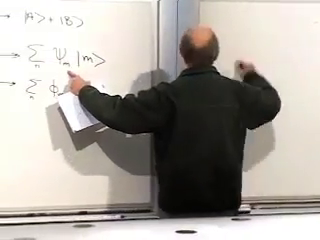
\includegraphics[width=0.68\textwidth]{lecture_07_figure_02.png}
\caption{스크린 기저에서 전개한 \(A\) 경로와 \(B\) 경로의 각각의 상태.}
\lectureframe{00:05:39}
\end{figure}

\(B\)을 막으면 위치 \(m\)에서의 확률은
\begin{equation}
P_A(m)=|\psi_m|^2.
\end{equation}
\(A\)를 막으면,
\begin{equation}
P_B(m)=|\phi_m|^2.
\end{equation}
고전 확률이라면 두 구멍이 모두 열려 있을 때 이 두 결과를 더해야 한다고 볼 것이다. 그러나 양자역학에서는 먼저 진폭을 더한다.
\begin{equation}
|A\rangle+|B\rangle
\longrightarrow
\sum_m(\psi_m+\phi_m)|m\rangle.
\end{equation}
스크린의 특정 위치에서,
\begin{align}
P(m)
&=|\psi_m+\phi_m|^2 \\
&=|\psi_m|^2+|\phi_m|^2
  +\psi_m^*\phi_m+\phi_m^*\psi_m.
\end{align}

\begin{figure}[htbp]
\centering
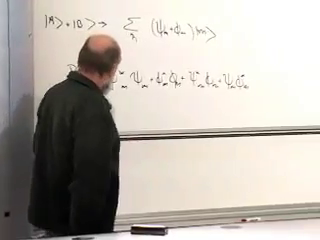
\includegraphics[width=0.70\textwidth]{lecture_07_figure_03.png}
\caption{스크린에서의 네 항 확률. 마지막 두 항은 간섭항이다.}
\lectureframe{00:09:21}
\end{figure}

대칭점에서는 \(\psi_m=\phi_m\)가 성립하여 두 대안이 서로 보강한다. 두 대안의 위상 차이가 \(\pi\)인 점, 즉 \(\psi_m=-\phi_m\)인 점에서는 확률이 사라진다. 어느 한 경로만으로도 그 점에 도달할 수 있지만, 두 경로를 모두 열면 전자가 그곳에 도달하지 못할 수 있다. 이제 다음 질문을 피할 수 없다. 어느 구멍을 통과했는지 기록하는 무언가가 생기면 무엇이 달라지는가?

\section{검출기와 얽히다}

상태 \(|u\rangle\)와 \(|d\rangle\)를 갖는 보조 2상태 계를 도입하자. 이 모형에서 이 계는 전자의 스핀이 아니라 최소한의 외부 장치다. 처음에 검출기는 작동하지 않은 상태다.
\begin{equation}
|0,d\rangle.
\end{equation}
\(A\)을 통과하면 검출기 상태가 뒤집히고, \(B\)을 통과하면 그대로 유지되도록 상호작용을 설정하자.
\begin{equation}
|0,d\rangle
\longrightarrow
|A,u\rangle+|B,d\rangle.
\end{equation}
전자가 구멍을 지난 뒤에는 보조 스핀과 더 이상 상호작용하지 않는다. 따라서 두 갈래는 다음과 같이 전파되고,
\begin{align}
|A,u\rangle &\longrightarrow \sum_m\psi_m|m,u\rangle, \\
|B,d\rangle &\longrightarrow \sum_m\phi_m|m,d\rangle,
\end{align}
최종 상태는 다음과 같다.
\begin{equation}
|\Psi\rangle
=\sum_m\left(\psi_m|m,u\rangle+\phi_m|m,d\rangle\right).
\end{equation}
이제 경로와 검출기의 기록이 얽혀 있다. 검출기를 읽으면 어느 구멍을 통과했는지 알 수 있다.

\begin{classroomqa}
\lecturetimestamp{00:13:24}
\audiencequestion{스핀이 뒤집히면 파동 묶음은 이미 붕괴한 것인가?}
\lecturerresponse{전자만 놓고 보면 경로 대안들이 더는 간섭하지 않는다는 뜻으로 붕괴라는 표현을 쓸 수 있다. 그러나 전자--검출기 전체 계에서는 어느 갈래도 버려지지 않았다. 상태는 여전히 \(|A,u\rangle+|B,d\rangle\)이다. 장치까지 포함하면 \emph{전자가 붕괴했다}는 표현은 계--장치의 얽힘이 형성되었다는 정확한 표현으로 대체된다.}
\end{classroomqa}

보조 스핀은 편리한 지시자일 뿐이다. 작동한 장치와 작동하지 않은 장치, 방출된 광자와 방출되지 않은 광자, 또는 서로 구별되는 다른 어떤 두 기록 상태도 같은 역할을 할 수 있다.

\begin{classroomqa}
\lecturetimestamp{00:15:17}
\audiencequestion{금속판을 통과하면 언제나 경로 기록이 남는가?}
\lecturerresponse{반드시 그렇지는 않다. 중요한 것은 상호작용으로 판이 구별 가능한 최종 상태에 놓이는가이다. 판에 여기 에너지 간격이 있고 전자의 에너지가 판을 여기시키기에 충분하지 않다면, 지속되는 내부 흔적이 남지 않을 수도 있다. 상호작용만으로는 충분하지 않다. 두 대안이 구별 가능한 기록과 상관관계를 이루어야 한다.}
\end{classroomqa}

\begin{classroomqa}
\lecturetimestamp{00:16:29}
\audiencequestion{판의 반동으로 전자가 위쪽과 아래쪽 중 어느 구멍을 통과했는지 알 수 있는가?}
\lecturerresponse{서로 반대 방향의 운동량 충격이 판을 충분히 구별 가능한 상태로 만들 때만 가능하다. 위치가 잘 국소화된 판은 이미 폭이 넓은 운동량 파동함수를 갖는다. 위아래로 조금씩 이동한 상태는 거의 완전히 겹칠 수 있으므로, 반동 상태들은 직교하지 않으며 경로를 확실하게 알려 주지 못한다. 여기서 불확정성 원리가 간섭을 보호한다.}
\end{classroomqa}

부분적인 기록도 가능하다. 검출기가 아주 약하게 밀려나면 두 최종 기록 상태가 직교하지 않을 수 있다. 이 경우 간섭은 사라지는 대신 약해진다. 형식적으로 계산하기 위해 우선 완전 측정이라는 극한적인 경우를 생각하자.
\begin{equation}
\langle u|d\rangle=0.
\end{equation}

\section{사영 연산자로 계산하기}

이제 검출기 결과는 묻지 않고 전자가 스크린의 특정 위치 \(m\)에 도달할 확률을 계산하자. 결합 힐베르트 공간에서 \emph{전자 위치가 \(m\)}이라는 성질은 다음 두 상태가 생성하는 2차원 부분공간에 해당한다.
\begin{equation}
|m,u\rangle,\qquad |m,d\rangle.
\end{equation}
이에 대응하는 사영 연산자는
\begin{equation}
\Pi_m
=|m,u\rangle\langle m,u|
 +|m,d\rangle\langle m,d|.
\end{equation}

\begin{figure}[htbp]
\centering
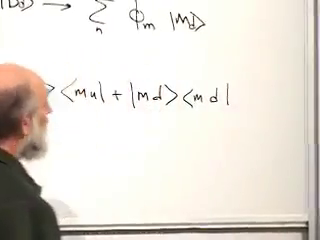
\includegraphics[width=0.66\textwidth]{lecture_07_figure_04.png}
\caption{두 직교 검출 기록에 대해 합한, 스크린의 특정 위치로의 사영 연산자.}
\lectureframe{00:22:04}
\end{figure}

확률 공리에 따르면
\begin{equation}
P(m)=\langle\Psi|\Pi_m|\Psi\rangle.
\end{equation}
합을 풀어 쓰면,
\begin{align}
P(m)
&=
\sum_{n,n'}
\left(\psi_n^*\langle n,u|+\phi_n^*\langle n,d|\right)
\notag\\
&\quad\times\Pi_m
\notag\\
&\quad\times
\left(\psi_{n'}|n',u\rangle+\phi_{n'}|n',d\rangle\right).
\end{align}
위치에 대한 내적은 \(n=m=n'\)을 요구한다. 이어서 검출기 내적에 따라 어떤 항이 남는지가 결정된다.
\begin{align}
\langle u|u\rangle&=1,
&
\langle d|d\rangle&=1,
&
\langle u|d\rangle&=\langle d|u\rangle=0.
\end{align}
따라서,
\begin{equation}
P(m)=|\psi_m|^2+|\phi_m|^2.
\end{equation}

교차항은 임의로 없앤 것이 아니다. 확장된 상태 공간에서 두 경로 진폭이 서로 직교하는 벡터와 곱해지기 때문에 사라진다. 간섭하려면 대안들이 스크린의 종착점에서만 일치해서는 안 된다. 기록을 담고 있는 모든 자유도에서도 일치해야 한다.

\section{무엇을 측정이라고 하는가?}

이 간결한 스핀 모형은 일반적인 규칙을 보여 준다. 계의 대안들과 장치의 구별 가능한 상태들 사이에 상관관계를 형성하는 상호작용이 일어날 때 측정이 성립한다. 다음 사례들로 이 규칙을 살펴보자.

\begin{classroomqa}
\lecturetimestamp{00:26:53}
\audiencequestion{스핀을 대칭적으로 배치하고 어느 구멍을 통과하든 뒤집히게 하면 어떻게 되는가?}
\lecturerresponse{그러면 두 갈래 모두 같은 기록 \(|A,u\rangle+|B,u\rangle=(|A\rangle+|B\rangle)\otimes|u\rangle\)을 갖는다. 검출기 상태는 인수분해되어 경로 정보를 알려 주지 않으므로 간섭 무늬는 그대로 남는다.}
\end{classroomqa}

\begin{figure}[htbp]
\centering
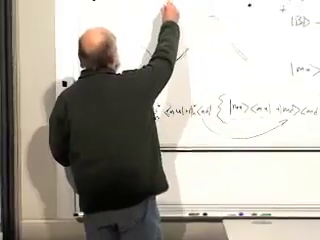
\includegraphics[width=0.68\textwidth]{lecture_07_figure_05.png}
\caption{대칭 위치에 둔 검출기가 두 경로에 똑같이 반응하도록 한 칠판의 변형 사례.}
\lectureframe{00:27:14}
\end{figure}

\begin{figure}[htbp]
\centering
\begin{tikzpicture}[scale=1.0]
\fill (-2,0) circle (1.5pt);
\node[left] at (-2,0) {$0$};
\fill (-0.7,0.9) circle (1.5pt);
\node[left] at (-0.8,0.9) {$A$};
\fill (-0.7,-0.9) circle (1.5pt);
\node[left] at (-0.8,-0.9) {$B$};
\draw (-2,0) -- (-0.7,0.9);
\draw (-2,0) -- (-0.7,-0.9);
\draw (-0.7,0.9) -- (2.0,0.5);
\draw (-0.7,-0.9) -- (2.0,-0.5);
\draw (2.2,-1.4) -- (2.2,1.4);
\node[right] at (2.2,0) {screen};
\fill (0.1,1.55) circle (1.5pt);
\node[above] at (0.1,1.55) {detector};
\draw[dashed] (0.1,1.45) -- (-0.15,0.72);
\draw[dashed] (0.1,1.45) -- (-0.15,-0.72);
\end{tikzpicture}
\caption{대칭적인 검출기 배치를 깔끔하게 재구성한 그림. 두 경로에서 검출기 상태는 동일하다.}
\end{figure}

\begin{classroomqa}
\lecturetimestamp{00:27:55}
\audiencequestion{간섭이 사라지려면 누군가 실제로 보조 스핀을 읽어야 하는가?}
\lecturerresponse{아니다. 전자는 이미 경로와 스핀 사이에 상관관계를 형성했다. 검출기를 초기화하고 전자를 한 번에 하나씩 보내면서 스크린에 도달한 위치 분포만 살펴볼 수 있다. 아무도 스핀을 읽지 않더라도 간섭 무늬는 사라진다. 중요한 것은 기록의 존재이지, 사람이 그 기록을 인식하는지가 아니다.}
\end{classroomqa}

\begin{classroomqa}
\lecturetimestamp{00:29:36}
\audiencequestion{충분히 가벼운 반동 판이라면 간섭을 없앨 수 있는가?}
\lecturerresponse{반동으로 두 경로에서 판이 직교하는 운동량 상태에 놓인다면 그렇다. 이동한 파동 묶음들이 여전히 겹친다면 간섭은 부분적으로만 사라진다. 기준은 질량 자체가 아니라 판의 최종 상태들이 구별 가능한가이다.}
\end{classroomqa}

복사도 불완전한 기록 장치가 될 수 있다. 가속된 하전 입자는 광자를 방출할 수 있다. \(A\) 부근에서 방출된 복사는 \(B\) 부근에서 방출된 복사와 같은 상태가 아닐 수 있으므로, 전자기장은 경로 정보를 보유할 수 있다. 천천히 편향된 전자의 경우 방출 확률은 작을 수 있다. 강의에서는 대략 백 번 중 한 번 일어나는 예시적 추산을 든다. 더 큰 가속은 복사와 그에 따른 대비 감소의 가능성을 높인다. 핵심은 정성적인 점이다. 관측되지 않은 광자도 결맞음을 가져갈 수 있다.

\begin{classroomqa}
\lecturetimestamp{00:32:00}
\audiencequestion{대비가 불완전한 실제 실험에서 간섭 확률은 어떻게 추론하는가?}
\lecturerresponse{실험을 여러 번 반복하고 상대도수로 스크린 분포를 추정한다. 표본 수가 유한하고 환경에 기록이 남으면 명목상 어두운 영역에서도 잔여 계수가 나타난다. 시행 횟수가 늘수록 추론한 확률 분포는 개선되며, 결맞음을 깨뜨리는 과정은 물리적인 간섭 무늬 대비를 낮춘다.}
\end{classroomqa}

\begin{classroomqa}
\lecturetimestamp{00:33:13}
\audiencequestion{경로를 알아낼 가능성만 있어도 간섭이 모두 사라지는가?}
\lecturerresponse{완전히 구별할 수 있으면 간섭은 완전히 사라진다. 정보가 부분적이면 간섭도 부분적으로만 줄어든다. 검출기가 조금만 회전하면 서로 직교하지 않는 두 기록 상태가 남는다. 따라서 검출기를 읽으면 한 경로가 다른 경로보다 더 가능성이 높아지지만 확실해지지는 않는다. 이에 따라 간섭 무늬는 지워지는 대신 흐려진다.}
\end{classroomqa}

\(|E_A\rangle\)와 \(|E_B\rangle\)를 임의의 기록 상태라고 하자. 스크린에서 결합 상태는 다음과 같이 쓸 수 있다.
\begin{equation}
|\Psi\rangle
=\sum_m\left(
\psi_m|m\rangle|E_A\rangle
+\phi_m|m\rangle|E_B\rangle
\right).
\end{equation}
기록 계를 무시하면,
\begin{align}
P(m)
&=|\psi_m|^2+|\phi_m|^2 \\
&\quad
+\psi_m^*\phi_m\langle E_A|E_B\rangle
+\phi_m^*\psi_m\langle E_B|E_A\rangle.
\end{align}
따라서 겹침 \(\langle E_A|E_B\rangle\)은 결맞음 인자다. 기록이 동일하면 간섭이 온전히 보존되고, 서로 직교하면 간섭이 사라지며, 겹침이 그 중간이면 가시도도 중간값을 갖는다.

\begin{classroomqa}
\lecturetimestamp{00:34:12}
\audiencequestion{광자는 가끔만 방출된다면, 광자가 방출된 경우만 골라 보면 어떻게 되는가?}
\lecturerresponse{그렇게 선택한 부분 앙상블에서는 일반적으로 간섭이 더 약하다. 광자가 경로 정보를 담기 때문이다. 간섭이 완전히 사라지지는 않을 수 있다. 두 구멍에서 방출된 광자 파동 묶음끼리 겹칠 수 있으므로 복사 기록도 완벽하게 직교하지 않을 수 있다.}
\end{classroomqa}

환경의 충돌은 이 메커니즘을 거시적 규모로 확대한다. 공기 분자, 주변 광자, 주위 물질은 거시적인 위치에 대한 기록을 끊임없이 얻는다. 사람이나 달이 결맞는 위치 중첩 상태로 눈에 띄게 퍼져 있는 상태로 남지는 않는다. 질량이 클수록 자유로운 퍼짐은 느려지고, 끊임없이 일어나는 환경과의 얽힘은 거시적으로 떨어진 대안 사이의 관측 가능한 간섭을 억제한다.

\begin{classroomqa}
\lecturetimestamp{00:36:02}
\audiencequestion{이것은 단순히 \emph{파동 묶음 붕괴}라는 말을 또 한 번 쓰는 데 그치지 않고, 이미 측정 이론을 제시하는 것인가?}
\lecturerresponse{여기서는 의도적으로 정확하게 설정한 예에서 그 메커니즘을 보여 준다. 전자만 기술할 때 붕괴는 비대각 \(\psi^*\phi\) 항을 버린다는 뜻이다. 복합계를 기술하면 임의로 항을 삭제할 필요가 없다. 직교하는 장치 상태와의 얽힘으로 인해 전자만을 측정하는 실험에서는 해당 항들을 이용할 수 없게 된다. 더 복잡한 사례도 이 구조로 되돌아가 살펴보아야 한다.}
\end{classroomqa}

\begin{classroomqa}
\lecturetimestamp{00:38:04}
\audiencequestion{경로를 휘게 하는 중력장이 복사에 대한 논증이나 간섭 규칙을 자연스럽게 바꿀 수 있는가?}
\lecturerresponse{복사의 세부 양상은 달라질 수 있고, 양자역학은 경로를 측정하기 전 입자의 단일한 명확한 궤적을 부여하지 않는다. 그러나 일반적인 결론은 달라지지 않는다. 구별 가능한 경로 정보를 보유하는 자유도만 간섭을 억제한다. 더 구체적으로 답하려면 실제 장치를 먼저 명시해야 한다.}
\end{classroomqa}

\begin{classroomqa}
\lecturetimestamp{00:39:44}
\audiencequestion{이 간섭은 고전 전자기파의 간섭과 다른가?}
\lecturerresponse{광자가 많이 있을 때 관측되는 무늬는 전자기장의 보통 파동 간섭과 일치한다. 단일 입자 실험은 더 근본적인 양자적 설명을 보여 준다. 광자와 전자는 개별 사건으로 도달하지만, 양자 진폭은 간섭한다. 전자의 경우 관련된 파동은 전자기파가 아니라 전자 파동함수다.}
\end{classroomqa}

\begin{classroomqa}
\lecturetimestamp{00:40:45}
\audiencequestion{초기 파동 중 \(A\)과 \(B\) 사이를 향한 부분은 어떻게 되는가?}
\lecturerresponse{이 의도적으로 이산화한 모형에서는 장벽의 나머지 부분이 막혀 있다. 그쪽을 향한 부분은 반사되므로 투과된 스크린 진폭에 기여하지 않는다. 이 모형은 투과하는 두 대안을 분리해 다룰 뿐, 실제 빔에 운동량 성분이 두 개뿐이라고 주장하지는 않는다.}
\end{classroomqa}

\section{고양이, 스크린, 그리고 이동 가능한 경계}

같은 수학은 Schr\"odinger의 고양이에도 적용된다. 총의 상태를 발사되지 않은 상태와 발사된 상태 \(|U\rangle\)와 \(|F\rangle\)로, 고양이의 상태를 살아 있는 상태와 죽은 상태 \(|L\rangle\)와 \(|D\rangle\)로 나타내자. 살아 있는 고양이와 발사되지 않은 총에서 시작하면 상호작용으로 다음 상태가 만들어질 수 있다.
\begin{equation}
|\Psi_{\mathrm{cat}}\rangle
=\alpha|L,U\rangle+\beta|D,F\rangle.
\end{equation}
고양이만의 상태는 결맞는 상태 \(\alpha|L\rangle+\beta|D\rangle\)가 아니다. 고양이는 대안을 기록한 총과 얽혀 있다. 총을 보면 고양이의 어느 갈래인지 알 수 있으며, 직교하는 총의 기록은 고양이 계에서 살아 있음--죽음 사이의 일반적인 간섭을 없앤다.

\begin{classroomqa}
\lecturetimestamp{00:41:18}
\audiencequestion{고양이 자체가 살아 있는 상태와 죽은 상태의 중첩에 있는가?}
\lecturerresponse{간단히 고립된 계로 보았을 때는 그렇지 않다. 고양이--총 복합계는 발사되지 않은 총과 살아 있는 고양이, 발사된 총과 죽은 고양이라는 상관된 대안들의 중첩 상태다. 고양이 계는 기록을 담은 총과 얽혀 있으며, 이는 전자 경로가 보조 스핀과 얽힌 것과 정확히 같다.}
\end{classroomqa}

최종 스크린도 측정 장치로 다루어야 한다. 위치 \(m\)에 도달한 전자는 사진 건판의 입자를 검게 만들거나, 섬광체에서 광자를 방출시키거나, 나란히 놓인 국소 2상태 장치 중 하나의 상태를 뒤집을 수 있다. 이렇게 도착 위치와 상관된 표지가 남는다.

\begin{classroomqa}
\lecturetimestamp{00:43:38}
\audiencequestion{상태 벡터만 영원히 다루는 대신 최종 스크린에서 확률을 말해도 되는 이유는 무엇인가?}
\lecturerresponse{확률 공리는 성질 \emph{도착 위치가 \(m\)}일 확률로 \(\langle\Pi_m\rangle\)을 부여한다. 물리적인 실험을 완성하려면 스크린에 위치 기록이 남아야 한다. 사영 연산자가 확률을 주고, 건판의 흑화나 섬광 또는 국소 검출기의 상태 변화가 수집하려는 통계를 만들어 내는 측정을 실현한다.}
\end{classroomqa}

\begin{classroomqa}
\lecturetimestamp{00:45:00}
\audiencequestion{스크린에서의 측정은 이야기하면서 \(A\)나 \(B\)를 통과할 확률은 왜 다루지 않는가?}
\lecturerresponse{경로 확률은 경로 기록 장치를 설치해야만 부여하고 검증할 수 있다. 기록이 없으면 대안들은 결맞은 상태를 유지하므로 진폭으로 더해야 한다. 스크린에는 위치 감응 장치가 있다고 가정한다. 차이는 특별한 시간에 있는 것이 아니라 해당 측정 상호작용을 마련했는지에 있다.}
\end{classroomqa}

계와 장치 사이의 경계는 옮길 수 있다. 기록 상태 \(|O_u\rangle\)와 \(|O_d\rangle\)를 갖는 관찰자를 포함하면,
\begin{equation}
|A,u\rangle+|B,d\rangle
\longrightarrow
|A,u,O_u\rangle+|B,d,O_d\rangle.
\end{equation}
또 다른 관찰자도 차례로 첫 번째 관찰자와 상관관계를 이룰 수 있다. 고양이 상자 안의 연기, 총, 고양이, Schr\"odinger, 비그너를 모두 더 긴 얽힘 사슬에 포함할 수 있다. 경계를 어디에 그리든 상관관계는 서로 일치해야 한다. 비그너가 나중에 Schr\"odinger에게 무엇을 보았는지 물으면 두 사람의 기록은 서로 일치한다.

\begin{classroomqa}
\lecturetimestamp{00:47:24}
\audiencequestion{계는 정확히 어디에서 끝나고 측정하는 관찰자는 어디서 시작하는가?}
\lecturerresponse{양자역학은 편리한 경계를 하나로 정해 주지 않는다. 전자만 기술하는 설명에서 붕괴를 적용할 수도 있고, 검출기를 포함한 더 큰 설명에서 붕괴를 적용할 수도 있으며, 관찰자까지 포함해 얽힌 상태를 다시 확장할 수도 있다. 물리적으로 필요한 것은 접근 가능한 모든 확률과 기록이 서로 일치하는 것이지, 하나의 유일한 기술상 경계가 아니다.}
\end{classroomqa}

\begin{classroomqa}
\lecturetimestamp{00:49:47}
\audiencequestion{경로를 측정하면 사건을 교란하기 때문에 불확정성 원리가 관련되는가?}
\lecturerresponse{그렇다. 반동 사례에서 그 관련성이 명확히 드러난다. 판의 위치를 국소화하면 운동량에 불확정성이 생겨 경로에 따라 작은 충격이 서로 구별되지 않을 수 있다. 더 일반적으로 양자 측정은 계--장치의 얽힘으로 상태가 변해야 비로소 완료되며, 그 변화는 이후의 간섭을 바꿀 수 있다.}
\end{classroomqa}

이 점에서 고전적인 이상과 뚜렷이 대비된다. 고전적으로는 측정을 임의로 약하게 하여 교란은 무시할 만큼 작게 유지하면서 정보를 얻을 수 있다고 생각한다. 여기서는 경로 정보를 얻으려면 장치와 상관관계를 형성해야 한다. 이는 결합 상태를 실제로 변화시키며, 이후 간섭 실험의 결과도 바꾼다.

\begin{classroomqa}
\lecturetimestamp{00:52:06}
\audiencequestion{\(A\)과 \(B\) 사이의 거리가 매우 커지면 어떻게 되는가?}
\lecturerresponse{보편적으로 적용되는 새로운 규칙은 없다. 이 광원과 장벽의 배치에서는 아주 멀리 떨어진 구멍에 도달하는 진폭 자체가 작아져 대부분의 입자가 막힌 부분에 부딪힐 수 있다. 이런 장치 의존적인 \(\psi_m\)와 \(\phi_m\)의 변화 외에는, 거리만으로 결맞음의 유지 여부가 결정되지 않는다.}
\end{classroomqa}

\begin{classroomqa}
\lecturetimestamp{00:53:04}
\audiencequestion{양자 시간 변화의 선형성은 근본적으로 정확한가? 자연이 선형성을 따르는 이유는 무엇인가?}
\lecturerresponse{선형성은 양자역학의 경험적 토대다. 작은 비선형 수정은 논리적으로 일관된 이론을 만들기 어렵고 이론의 구조를 망가뜨리는 경향이 있다. 물리적 명제들이 고전적인 집합이 아니라 부분공간의 논리를 따르는 더 깊은 이유는 여기서 제시하지 않는다. 강의에서는 이를 자연의 사실로 다룬다.}
\end{classroomqa}

\begin{classroomqa}
\lecturetimestamp{00:54:53}
\audiencequestion{나중의 관측으로 앞서 일어난 경로를 알아내 간섭 여부를 바꿀 수 있는가?}
\lecturerresponse{나중의 관측으로 경로를 알아낼 수 있다면, 어떤 물리적 자유도가 경로 의존적인 기록을 보존했어야 한다. 그 기록은 누군가 읽을 필요 없이 이미 결맞음에 영향을 준다. 인과율은 여전히 지켜져야 하며, 전체 시공간 배치와 장치를 명시하지 않고서는 추상적인 지연 선택 주장을 결론 내릴 수 없다.}
\end{classroomqa}

\begin{classroomqa}
\lecturetimestamp{00:56:47}
\audiencequestion{구멍 바로 뒤에 기포 상자를 놓으면 어떻게 되는가?}
\lecturerresponse{나오는 두 경로를 구별하는 궤적은 명백한 표지이므로 간섭을 없앤다. 얇은 경로 기록층만으로도 충분하다. 하류의 장치가 앞서 통과한 구멍을 추론할 만큼 충분한 정보를 보존하지 않는다면, 그 장치가 자동으로 경로 검출기 역할을 하지는 않는다.}
\end{classroomqa}

\begin{classroomqa}
\lecturetimestamp{00:59:29}
\audiencequestion{세상이 이미 강하게 얽혀 있다면 간섭 실험은 어떻게 얽히지 않은 계들로 시작할 수 있는가?}
\lecturerresponse{실험 준비 과정에서 관련 자유도를 충분히 격리하거나 초기화하거나 조건화하여 대안들이 같은 환경 기록을 가진 상태로 시작하게 해야 한다. 앞선 기포 상자의 궤적이 경로와 계속 상관되어 있다면 이를 단순히 무시할 수 없다. 간섭을 얻으려면 제어하는 계와 관련 기록 장치 사이의 초기 관계가 곱 상태에 가까워야 한다.}
\end{classroomqa}

\begin{classroomqa}
\lecturetimestamp{01:01:04}
\audiencequestion{측정 뒤에는 실제로 어떻게 얽힘을 해소하는가?}
\lecturerresponse{관측 결과 하나를 확정해 조건을 건다. 스핀이 위쪽으로 측정되었다면 관찰자는 갈래 \(|A,u\rangle\)를 유지하고 나머지 대안은 작업 설명에서 버린다. 이렇게 조건화한 곱 상태를 새로운 출발점으로 삼을 수 있다. 관찰자까지 포함한 전체 상태는 계속 얽혀 있을 수 있지만, 기록된 결과를 기준으로 보면 선택된 준비 상태는 명확하다.}
\end{classroomqa}

이런 중첩된 위계가 모든 해석상의 질문을 해결해 주지는 않지만, 조작적 일관성을 분명하게 보여 준다. 계, 검출기, 관찰자, 관찰자의 관찰자를 모두 포함할 수 있다. 기술의 경계를 어디에 두든 올바르게 상관된 기록들은 나중에 서로 모순되지 않는다.

\section{얽힘에서 엔트로피로}

측정에 관해 계획보다 더 깊이 살펴보았지만, 이로써 다음 질문이 드러났다. 얽힘의 정도를 어떻게 측정할 수 있을까? 곱 상태
\begin{equation}
|u\rangle\otimes|u\rangle
\end{equation}
에 있는 두 스핀은 얽혀 있지 않다. 각 부분계에는 각각의 명확한 상태가 있으며, 하나를 관측해도 다른 하나에 대한 새로운 정보는 얻지 못한다. 얽힌 상태는 이렇게 인수분해되지 않는다. 얽힘 엔트로피는 이를 정량적으로 판별하는 표준적인 방법이지만, 먼저 보통의 엔트로피 개념을 살펴본 다음 양자적 형태를 다루어야 한다.

\section{고전 엔트로피와 정보의 부족}

유한한 \(N\)개의 가능한 상태를 갖는 고전계를 생각해 보자. 여기서 엔트로피는 계 자체와 그 계에 대해 우리가 가진 지식이 함께 정하는 성질이다. 계가 \(n\)개의 상태 중 하나에 있다는 것만 알고 있고, 각 상태가 똑같이 가능하다고 하자. 그러면
\begin{equation}
S=\log n.
\end{equation}
\(n=1\)이면 상태를 알고 있으므로 \(S=0\)이다. \(n=N\)이면 상태 공간 자체 외에는 아무것도 알지 못하며 엔트로피는 최대인 \(S_{\max}=\log N\)이다.

로그는 서로 독립적인 예--아니오 선택을 덧셈으로 센다. \(M\)개의 고전 스핀에는 \(2^M\)개의 배열이 있으므로,
\begin{equation}
\log(2^M)=M\log 2.
\end{equation}
로그의 밑을 무엇으로 택하느냐에 따라 달라지지만, 엔트로피는 기술에서 빠져 있는 이진 정보의 양을 센다.

일반적인 확률 분포 \(p_i\)에 대해서는 다음 정의를 쓴다.
\begin{equation}
S=-\sum_i p_i\log p_i.
\end{equation}

\begin{classroomqa}
\lecturetimestamp{01:14:17}
\audiencequestion{엔트로피 공식에는 왜 마이너스 부호가 있나요?}
\lecturerresponse{양의 확률은 모두 \(0<p_i\leq 1\)을 만족하므로, \(\log p_i\leq 0\)입니다. 마이너스 부호는 엔트로피가 음수가 되지 않게 합니다. \(p_i=0\)에서는 그 항을 극한 \(p_i\log p_i\to0\)으로 정의합니다.}
\end{classroomqa}

등확률 분포
\begin{equation}
p_i=
\begin{cases}
1/n, & i\in\mathcal N,\\
0, & i\notin\mathcal N,
\end{cases}
\qquad |\mathcal N|=n,
\end{equation}
에서는 일반식이 다음과 같이 된다.
\begin{align}
S
&=-n\left(\frac1n\right)\log\left(\frac1n\right)\\
&=\log n.
\end{align}
따라서 기본적인 계수 정의를 재현한다. 한 상태에 확률 1로 집중된 분포에서는 \(S=0\)이다.

\begin{figure}[htbp]
\centering
\includegraphics[width=0.66\textwidth]{lecture_07_figure_07.png}
\caption{칠판에는 \(S=\log n\), 섀넌 공식, 등확률 분포를 통한 확인이 정리되어 있다.}
\lectureframe{01:16:08}
\end{figure}

\begin{classroomqa}
\lecturetimestamp{01:17:35}
\audiencequestion{\(N\)개의 상태를 갖는 계의 엔트로피는 얼마나 클 수 있으며, 그 경우 무엇을 알고 있는가?}
\lecturerresponse{최댓값은 \(\log N\)이며, 균등 분포 \(p_i=1/N\)에서 얻는다. 계가 무엇인지, 따라서 상태 공간이 무엇인지는 여전히 알고 있다. 모르는 것은 그 \(N\)개 상태 중 어느 상태에 있는지다.}
\end{classroomqa}

차이
\begin{equation}
I=S_{\max}-S
\end{equation}
는 이런 계수 방식으로 정의한 가용 정보다. 엔트로피와 정보는 같은 장부 정리의 양면이다. 엔트로피는 상태를 구별해 줄 수 있지만 우리가 이용할 수 없는 정보를 나타낸다.

\section{부분합: 합을 대신하는 양자 개념}

연산자 \(M\)와 임의의 완비 정규직교 기저 \(\{|i\rangle\}\)에 대해 다음과 같이 정의한다.
\begin{equation}
\operatorname{Tr}M
=\sum_i\langle i|M|i\rangle.
\end{equation}

\begin{figure}[htbp]
\centering
\includegraphics[width=0.68\textwidth]{lecture_07_figure_08.png}
\caption{대각 행렬 원소들의 합으로 쓴 부분합.}
\lectureframe{01:21:20}
\end{figure}

정의는 기저를 사용해 쓰여 있지만, 결과는 기저에 무관하다. 에르미트 연산자의 경우 고유기저를 택할 수 있으며, 이때는
\begin{equation}
\operatorname{Tr}M=\sum_i\lambda_i.
\end{equation}
고유값과 그 합은 연산자를 나타내는 데 사용한 좌표에 의존하지 않는다.

\begin{classroomqa}
\lecturetimestamp{01:23:04}
\audiencequestion{행렬을 대각형으로 나타내면 역행렬이 존재한다는 뜻인가요?}
\lecturerresponse{아닙니다. 대각형으로 나타내면 고윳값을 알 수 있지만, 가역성은 별개의 조건입니다. 대각행렬은 대각 원소인 고윳값이 모두 영이 아닐 때, 그리고 그때에만 가역입니다. 일부 고윳값이 영인 에르미트 행렬도 대각화할 수 있습니다.}
\end{classroomqa}

휴식 후에는 잠시 고전 확률로 돌아가겠습니다. 고전 관측가능량은 배치의 함수 \(f_i\)이고, 그 평균은 다음과 같습니다.
\begin{equation}
\langle f\rangle_{\mathrm{cl}}=\sum_i p_i f_i.
\end{equation}
양자 공식에서는 대안들에 대한 합을 트레이스로, 고전 함수를 연산자로, 확률분포를 밀도행렬로 바꾸어 표현합니다.

\section{통계적 혼합 상태와 밀도행렬}

어떤 사람이 정규직교 기저의 상태 가운데 하나로 계를 준비했지만, 어느 상태를 선택했는지는 알려주지 않는다고 합시다. 그 사람이 알려주는 것은 준비 확률---뿐입니다. 예를 들어 스핀을 위쪽 상태로 준비할 확률은 \(3/4\)이고 아래쪽 상태로 준비할 확률은 \(1/4\)입니다. 이는 다음과 같은 결맞은 중첩이 아닙니다.
\begin{equation}
\sqrt{\frac34}|u\rangle+\sqrt{\frac14}|d\rangle,
\end{equation}
상대 위상이 준비되지 않았기 때문입니다. 이는 확정된 상태들의 통계적 혼합입니다. 순수 상태를 알고 있더라도 양자 확률은 여전히 남습니다. 여기에는 어떤 순수 상태가 준비되었는지에 대한 불확실성이 추가로 있습니다.

\begin{figure}[htbp]
\centering
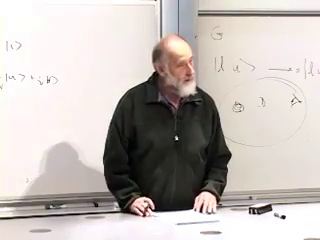
\includegraphics[width=0.66\textwidth]{lecture_07_figure_06.png}
\caption{지정된 켓에서 앙상블 기술로 넘어가는 개념적 전환.}
\lectureframe{01:29:43}
\end{figure}

상태 \(|i\rangle\)를 확률 \(\rho_i\)로 준비하면 밀도 연산자는 다음과 같습니다.
\begin{equation}
\rho=\sum_i\rho_i|i\rangle\langle i|.
\end{equation}
준비 기저에서는 다음과 같습니다.
\begin{equation}
\rho=
\begin{pmatrix}
\rho_1&0&0&\cdots\\
0&\rho_2&0&\cdots\\
0&0&\rho_3&\cdots\\
\vdots&\vdots&\vdots&\ddots
\end{pmatrix}.
\end{equation}

\begin{figure}[htbp]
\centering
\includegraphics[width=0.68\textwidth]{lecture_07_figure_09.png}
\caption{대각 밀도행렬과 그 정규화 조건.}
\lectureframe{01:32:12}
\end{figure}

고윳값은 실수이며 음이 아닌 값이고, 확률의 정규화 조건은 다음과 같습니다.
\begin{equation}
\operatorname{Tr}\rho=\sum_i\rho_i=1.
\end{equation}

\(F\)을 에르미트 관측가능량이라고 합시다. 앙상블의 기댓값은 다음과 같습니다.
\begin{equation}
\langle F\rangle=\operatorname{Tr}(F\rho).
\end{equation}

\begin{figure}[htbp]
\centering
\includegraphics[width=0.68\textwidth]{lecture_07_figure_10.png}
\caption{트레이스로 나타낸 기댓값 \(\langle F\rangle=\operatorname{Tr}(F\rho)\).}
\lectureframe{01:35:05}
\end{figure}

일반적인 가중평균을 얻으려면 \(\rho\)가 대각화된 기저에서 트레이스를 계산하고 항등 연산자의 분해를 대입하면 됩니다.
\begin{align}
\operatorname{Tr}(F\rho)
&=\sum_i\langle i|F\rho|i\rangle\\
&=\sum_{i,j}\langle i|F|j\rangle
               \langle j|\rho|i\rangle\\
&=\sum_i\rho_i\langle i|F|i\rangle.
\end{align}
따라서 각 순수 상태의 기댓값에는 그 상태가 준비되었을 확률이 가중치로 주어집니다.

트레이스에는 다음과 같은 순환 성질이 있습니다.
\begin{equation}
\operatorname{Tr}(AB)=\operatorname{Tr}(BA),
\end{equation}
\(A\)와 \(B\)가 서로 가환하지 않더라도 성립합니다. 따라서 \(\operatorname{Tr}(F\rho)=\operatorname{Tr}(\rho F)\)입니다.

\section{양자 엔트로피와 뒤로 미룬 결론}

밀도행렬의 엔트로피는 다음과 같습니다.
\begin{equation}
S(\rho)=-\operatorname{Tr}(\rho\log\rho).
\end{equation}
\(\log\rho\)와 같은 함수는 에르미트 양의 연산자의 고윳값을 통해 정의됩니다. 만약
\begin{equation}
\rho=\sum_i\rho_i|i\rangle\langle i|,
\end{equation}
라면,
\begin{equation}
\log\rho=\sum_{\rho_i>0}(\log\rho_i)|i\rangle\langle i|,
\end{equation}
따라서 다음과 같습니다.
\begin{equation}
S(\rho)=-\sum_i\rho_i\log\rho_i.
\end{equation}

\begin{figure}[htbp]
\centering
\includegraphics[width=0.68\textwidth]{lecture_07_figure_11.png}
\caption{고전 엔트로피 공식을 \(S=-\operatorname{Tr}(\rho\log\rho)\)로 다시 쓴 표현.}
\lectureframe{01:41:25}
\end{figure}

알려진 순수 상태의 밀도 연산자는 다음과 같습니다.
\begin{equation}
\rho_\psi=|\psi\rangle\langle\psi|,
\end{equation}
고윳값은 \(1,0,\ldots\)이므로 \(S(\rho_\psi)=0\)입니다. 이는 \(|\psi\rangle\)에 대한 모든 측정에서 결과가 확정되어 있다는 뜻은 아닙니다. 준비된 상태에 대해 추가적인 통계적 무지가 없다는 뜻입니다. 정반대의 경우는 다음과 같습니다.
\begin{equation}
\rho=\frac{I}{d}
\qquad\Longrightarrow\qquad
S(\rho)=\log d,
\end{equation}
여기서 \(d=\dim\mathcal H\)입니다. 최대 혼합 상태는 모든 직교 방향에 같은 가중치를 부여합니다.

얽힘과의 연관성은 이제 가까워졌지만, 아직 구체적으로 전개하지 않았습니다. 합성계 \(AB\)가 공동 상태에 있고 모든 실험이 \(A\)에만 한정된다고 하자. \(B\)를 무시한 채 \(A\)에서 얻을 수 있는 모든 기댓값을 재현하는 대상이 있어야 합니다. 그 대상이 \(A\)의 밀도행렬입니다. 공동 상태가 인수분해되면 \(A\)의 밀도행렬은 순수 상태이며 엔트로피는 영입니다. \(A\)와 \(B\)가 얽혀 있으면 \(A\)의 밀도행렬은 일반적으로 혼합 상태이며 엔트로피는 영이 아닙니다. 이 축약 밀도행렬을 구성하고 엔트로피를 계산하는 일은 다음 강의에서 다룰 내용입니다.

\graphicspath{{../../../generated_course_notes/supplementary/quantum_entanglement/2006_fall_part_1/chapters/lecture_08/}{../../../generated_course_notes/supplementary/quantum_entanglement/2006_fall_part_1/figures/}{../../../generated_course_notes/supplementary/quantum_entanglement/2006_fall_part_1/assets/}}
\chapter{축약 상태, 얽힘 엔트로피와 유니터리 시간 발전}

밀도 행렬은 처음에는 불완전한 준비를 자연스럽게 기술하는 대상으로 등장한다. 양자계가 준비되었지만, 어떻게 준비되었는지 정확히 알지 못하는 경우다. 얽힘은 같은 수학적 대상에 더 깊은 역할을 부여한다. 복합계의 상태를 완전히 알고 있더라도, 부분계에는 일반적으로 그 자체의 상태 벡터가 없다. 축약 밀도 행렬에는 국소적으로 예측할 수 있는 모든 것이 담겨 있다. 이를 성분으로 유도하고, 두 스핀 상태에 적용해 확인한 뒤, 엔트로피를 이용해 곱 상태와 얽힌 상태를 구분해 보겠다. 그런 다음 두 번째 질문, 즉 양자 상태가 시간에 따라 어떻게 변하는지 살펴보겠다. 내적의 보존으로부터 유니터리성, 에르미트 생성자, 그리고 Schr\"odinger 방정식을 얻는다.

\section{밀도 행렬과 불완전한 준비}

전자를 강한 자기장에 놓고 자기장 방향으로 정렬되도록 했다고 하자. 다른 사람이 자기장 방향을 정해 전자를 준비했지만, 그 방향을 우리에게 알려주지 않았다. 따라서 어떤 상태인지는 모르더라도 스핀은 완전히 확정된 순수 상태에 있을 수 있다. 가능한 준비 방법에 대한 확률 분포를 알고 있을 수도 있고, 아무것도 모를 수도 있다. 밀도 행렬 \(\rho\)은 바로 이런 종류의 불완전한 정보를 양자역학적으로 기술한다.

이에 대응하는 고전적 대상은 위상 공간의 확률 밀도 또는 이산적인 배치들에 대한 확률 분포다. 양자적 대상은 다음 세 가지 핵심 성질을 갖는 연산자다.
\begin{equation}
\rho^\dagger=\rho,
\qquad
\operatorname{Tr}\rho=1,
\qquad
\lambda_i\geq 0,
\end{equation}
여기서 \(\lambda_i\)는 \(\rho\)의 고윳값이다. 에르미트성에 따라 고윳값은 실수이고 정규직교 고유기저가 존재한다. 양의 정부호성에 따라 고윳값은 확률로 해석할 수 있으며, 정규화 조건은 다음과 같다.
\begin{equation}
\sum_{i=1}^{n}\lambda_i=1.
\end{equation}
\(\rho\)의 고유기저에서 \(\lambda_i\)은 \(i\)번째 고유상태에 부여된 확률이다.

완전한 무지는 힐베르트 공간에서 어느 방향도 특별히 선호되지 않는 경우다.
\begin{equation}
\rho_{\mathrm{max}}=\frac{1}{n}I.
\end{equation}
모든 고윳값은 \(1/n\)이다. 반대 극단인 완전한 지식은 정규화된 상태 \(\ket{\psi}\)로 나타내며,
\begin{equation}
\rho_\psi=\ket{\psi}\bra{\psi}.
\end{equation}
이는 \(\ket{\psi}\)가 생성하는 1차원 부분공간으로의 사영 연산자다.

\begin{classroomqa}
\lecturetimestamp{00:06:47}
\audiencequestion{서로 직교하지 않는 두 상태, 예를 들어 스핀 방향이 \(45^\circ\)만큼 벌어진 두 상태 중 하나를 절반씩 선택하는 준비로 기술할 수 있나요?}
\lecturerresponse{그런 준비 절차는 가능하지만, 그 두 가중치가 결과 밀도 행렬의 고윳값이 되는 것은 일반적으로 아니다. 먼저 사영 연산자들의 가중합을 만든 다음 대각화한다. 고윳값을 확률로 해석하는 명확한 의미는 \(\rho\)의 정규직교 고유기저에 해당하며, 준비자가 지정한 비직교 상태들에 반드시 대응하는 것은 아니다.}
\end{classroomqa}

\begin{classroomqa}
\lecturetimestamp{00:07:47}
\audiencequestion{순수 상태와 혼합 상태는 무엇으로 구별되는가?}
\lecturerresponse{순수 상태의 밀도 행렬에는 0이 아닌 고윳값이 하나 있으며, 그 값은 \(1\)이다. 혼합 상태에는 0이 아닌 고윳값이 둘 이상 있다. 오래된 문헌에서는 독일어 \emph{Gemisch}라는 단어를 사용했으며, 현대에는 간단히 \emph{혼합 상태}라고 한다.}
\end{classroomqa}

순수 상태 사영 연산자의 스펙트럼을 확인해 보자. 정규화 조건에 따라
\begin{equation}
\rho_\psi\ket{\psi}
=\ket{\psi}\braket{\psi}{\psi}
=\ket{\psi},
\end{equation}
따라서 \(\ket{\psi}\)는 고윳값이 \(1\)인 고유벡터다. \(\ket{\phi}\)가 \(\ket{\psi}\)와 직교하면,
\begin{equation}
\rho_\psi\ket{\phi}
=\ket{\psi}\braket{\psi}{\phi}
=0.
\end{equation}
그러므로 \(\ket{\psi}\)에 직교하는 모든 방향의 고윳값은 0이다.

\begin{figure}[htbp]\centering
\includegraphics[width=0.72\textwidth]{lecture_08_figure_06.png}\caption{순수 상태 밀도 행렬의 사영 연산자 작용: \(\rho\ket{\psi}=\ket{\psi}\)}\lectureframe{00:09:32}\end{figure}

\section{트레이스로부터 기대값 구하기}

밀도 행렬에 적용하는 조작적 규칙은 다음과 같다.
\begin{equation}
\overline{M}=\operatorname{Tr}(\rho M),
\end{equation}
여기서 \(M\)는 관측량이다. 두 인자에 대해 트레이스의 순환 성질을 적용하면 다음을 얻는다.
\begin{equation}
\operatorname{Tr}(\rho M)=\operatorname{Tr}(M\rho),
\end{equation}
이는 \(\rho\)와 \(M\)가 가환하는지 여부와 관계없다.

임의의 정규직교 기저 \(\{\ket{i}\}\)에서
\begin{equation}
\operatorname{Tr}X=\sum_i\bra{i}X\ket{i}.
\end{equation}
수치 값은 기저에 의존하지 않는다. 순수 상태의 경우,
\begin{align}
\overline{M}
&=\operatorname{Tr}\!\left(\ket{\psi}\bra{\psi}M\right) \\
&=\sum_i\braket{i}{\psi}\bra{\psi}M\ket{i} \\
&=\bra{\psi}M\left(\sum_i\ket{i}\bra{i}\right)\ket{\psi} \\
&=\bra{\psi}M\ket{\psi}.
\end{align}
항등 연산자의 분해식
\begin{equation}
\sum_i\ket{i}\bra{i}=I,
\end{equation}
을 대입하면 밀도 행렬 규칙은 익숙한 순수 상태 기대값으로 돌아간다.

\begin{figure}[htbp]\centering
\includegraphics[width=0.74\textwidth]{lecture_08_figure_07.png}\caption{순수 상태 사영 연산자에 대한 트레이스 계산과 항등 연산자의 분해식.}\lectureframe{00:14:25}\end{figure}

\begin{classroomqa}
\lecturetimestamp{00:14:38}
\audiencequestion{왼쪽에 있는 양은 \(\overline{M}\), 즉 \(M\)의 평균인가요?}
\lecturerresponse{그렇다. 트레이스는 연산자 \(M\) 자체가 아니라 스칼라인 기대값 \(\overline{M}\)이다.}
\end{classroomqa}

일반적인 밀도 행렬의 고유기저를 택하자.
\begin{equation}
\rho\ket{j}=\lambda_j\ket{j}.
\end{equation}
\(\rho\)와 \(M\) 사이에 완비 상태 집합을 삽입하면
\begin{align}
\overline{M}
&=\sum_i\bra{i}\rho M\ket{i} \\
&=\sum_{i,j}\bra{i}\rho\ket{j}\bra{j}M\ket{i} \\
&=\sum_{i,j}\lambda_j\delta_{ij}\bra{j}M\ket{i} \\
&=\sum_j\lambda_j\bra{j}M\ket{j}.
\end{align}
이는 보통의 가중 평균이다. \(\lambda_j\)는 \(j\)번째 고유상태일 확률이고, \(\bra{j}M\ket{j}\)은 그 상태에서 \(M\)의 기대값이다.

\begin{classroomqa}
\lecturetimestamp{00:18:12}
\audiencequestion{마지막 행렬 원소의 두 지표가 왜 모두 \(j\)가 되며, 여전히 합을 취하는 지표는 무엇인가요?}
\lecturerresponse{\(\rho\)는 이 기저에서 대각 행렬이므로 \(\bra{i}\rho\ket{j}=\lambda_j\delta_{ij}\)이고, 따라서 \(i=j\)인 항만 남는다. 원래의 이중 합은 단일 합으로 줄어들며, 이를 \(j\)에 대한 합이라고 할 수 있다. 더미 합산 지표의 이름에는 물리적 의미가 없다.}
\end{classroomqa}

\section{정보의 결핍으로서의 엔트로피}

고전적 확률 분포 \(\{p_i\}\)에 대해 다음과 같이 정의하자.
\begin{equation}
S=-\sum_i p_i\log p_i,
\end{equation}
여기서 \(0\log 0\)는 극한값 \(0\)으로 이해한다. 확률 하나가 \(1\)이고 나머지는 모두 사라지면 \(S=0\)이다. 즉, 상태를 알고 있는 것이다. 가능한 \(n\)가지 경우의 확률이 모두 같다면
\begin{equation}
p_i=\frac{1}{n},
\qquad
S=-n\left(\frac{1}{n}\log\frac{1}{n}\right)=\log n.
\end{equation}
따라서 확률 분포가 더 많은 유의미한 가능성에 걸쳐 퍼질수록 엔트로피가 커진다. 대략적으로 말해, 자연로그를 사용할 때 \(e^S\)은 비슷한 가중치를 갖는 상태의 유효 개수이다.

\begin{figure}[htbp]\centering
\includegraphics[width=0.68\textwidth]{lecture_08_figure_08.png}\caption{확률 분포의 엔트로피와 확률이 균등할 때의 값 \(S=\log n\).}\lectureframe{00:21:08}\end{figure}

밀도 행렬의 경우에도 같은 정의를 고윳값에 적용한다.
\begin{equation}
S(\rho)=-\sum_i\lambda_i\log\lambda_i
=-\operatorname{Tr}(\rho\log\rho).
\end{equation}
첫 번째 표현이 당장 필요한 식이고, 트레이스로 쓴 형태는 결과가 기저에 무관함을 강조한다.

\section{복합계와 국소 실험}

두 부분계 \(A\)와 \(B\)를 생각하자. 기저 벡터는 \(\ket{a,b}\)로 쓴다. \(A\)에 기저 상태가 \(N\)개 있고 \(B\)에 \(n\)개 있으면, 복합계에는 기저 상태가 \(Nn\)개 있다. 두 계가 서로 비슷할 필요는 없다. 하나는 두 상태를 가진 스핀이고 다른 하나는 세 상태를 가진 원자일 수 있다.

두 부분계의 가장 일반적인 순수 상태는 다음과 같다.
\begin{equation}
\ket{\Psi}
=\sum_{a,b}\psi(a,b)\ket{a,b},
\qquad
\sum_{a,b}|\psi(a,b)|^2=1.
\end{equation}
이제 앨리스가 부분계 \(A\)에만 작용하는 관측량 \(M_A\)를 측정한다고 하자. 복합 힐베르트 공간에서 그 연산자는 \(M_A\otimes I_B\)이다. 행렬 원소는 다음과 같다.
\begin{equation}
\bra{a',b'}M_A\otimes I_B\ket{a,b}
=\bra{a'}M_A\ket{a}\,\delta_{b'b}.
\end{equation}
\(B\) 지표는 연산자의 작용 대상이 아니다.

기대값을 전개해 쓰면 다음과 같다.
\begin{align}
\expect{M_A}
&=\bra{\Psi}M_A\otimes I_B\ket{\Psi} \\
&=\sum_{a',b'}\sum_{a,b}
\psi^*(a',b')\psi(a,b)
\bra{a'}M_A\ket{a}\delta_{b'b} \\
&=\sum_{a',a,b}
\psi^*(a',b)\psi(a,b)
\bra{a'}M_A\ket{a}.
\end{align}

\begin{classroomqa}
\lecturetimestamp{00:29:12}
\audiencequestion{브라의 지표에는 프라임이 붙고 켓의 지표에는 붙지 않는 이유가 무엇인가요?}
\lecturerresponse{행렬 원소를 계산하기 전에는 브라와 켓의 합이 서로 독립적이므로 각각 다른 더미 지표가 필요하다. 프라임은 브라의 지표와 켓의 지표를 구분한다. 그다음 연산자와 내적에 따라 어떤 지표들이 일치해야 하는지가 정해진다.}
\end{classroomqa}

\(a\)와 \(a'\)를 고정하고 \(b\)에 대한 합을 계산하자. 그 결과는 부분계 \(A\)의 행렬이다.
\begin{equation}
\boxed{
\rho_A(a,a')
=\sum_b\psi(a,b)\psi^*(a',b)
}.
\end{equation}
이것은 \(A\)의 축약 밀도 행렬이며, 동등하게는 순수 상태 사영 연산자를 \(B\)에 대해 부분 트레이스한 것이다.
\begin{equation}
\rho_A=\operatorname{Tr}_B\ket{\Psi}\bra{\Psi}.
\end{equation}
그러면 국소 기대값은 다음과 같이 된다.
\begin{equation}
\expect{M_A}
=\sum_{a,a'}\rho_A(a,a')\bra{a'}M_A\ket{a}
=\operatorname{Tr}_A(\rho_A M_A).
\end{equation}

\begin{figure}[htbp]\centering
\includegraphics[width=0.76\textwidth]{lecture_08_figure_09.png}\caption{\(B\) 지표를 합산해 없애면 \(A\) 지표 두 개를 가진 행렬이 남는다.}\lectureframe{00:33:50}\end{figure}

\begin{classroomqa}
\lecturetimestamp{00:35:39}
\audiencequestion{국소 관측량은 부분계 \(B\)에 대한 항등 연산자일 뿐인가요?}
\lecturerresponse{그렇다. \(M_A\otimes I_B\)는 \(A\) 좌표를 바꿀 수 있지만, \(b\)를 바꾸지도 않고 그 값에 의존하지도 않는다. 그래서 \(B\) 공간에서의 행렬 원소는 \(\delta_{b'b}\)이다.}
\end{classroomqa}

따라서 \(A\)에 국한된 실험에 대한 모든 예측은 \(\rho_A\)에 담겨 있다. 밥은 자신의 부분계를 측정할 필요가 없다. \(B\) 자유도를 사용하지 않기로 하는 것만으로도 앨리스의 기술은 밀도 행렬 형식이 된다.

\section{순수한 전체계와 혼합된 부분계}

결합된 계는 순수 상태 \(\ket{\Psi}\)에 있지만, \(\rho_A\)에는 일반적으로 0이 아닌 고윳값이 여러 개 있다. 전체를 완전히 알고 있다고 해서 각 부분의 상태 벡터까지 알 수 있는 것은 아니다. 고양이와 총은 하나의 얽힌 상태 벡터로 기술될 수 있으며, 이때 고양이만은 축약 밀도 행렬로 기술된다.

\begin{classroomqa}
\lecturetimestamp{00:38:25}
\audiencequestion{\(\operatorname{Tr}(M\rho)\)를 \((\operatorname{Tr}M)(\operatorname{Tr}\rho)\)로 바꿔 써도 되나요?}
\lecturerresponse{안 된다. 곱의 트레이스는 일반적으로 각 인자의 트레이스를 곱한 것과 같지 않다. 순환성에 따라 \(\operatorname{Tr}(M\rho)=\operatorname{Tr}(\rho M)\)라고 쓸 수는 있지만, 트레이스가 인자별로 분해되지는 않는다.}
\end{classroomqa}

\begin{classroomqa}
\lecturetimestamp{00:38:49}
\audiencequestion{처음에 기저 상태 \(\ket{a,b}\)만으로 시작했나요, 아니면 가장 일반적인 순수 상태로 시작했나요?}
\lecturerresponse{복합계의 가장 일반적인 순수 상태로 시작했다. \(\ket{\Psi}=\sum_{a,b}\psi(a,b)\ket{a,b}\). 하나의 \(\ket{a,b}\)는 기저 벡터 하나일 뿐이다. 놀라운 점은 이렇게 완전히 지정된 복합계의 벡터조차 혼합된 축약 상태를 만들 수 있다는 것이다.}
\end{classroomqa}

고전역학과의 차이는 뚜렷하다. 복합계에 대한 고전적 정보를 완전히 알면 각 좌표가 정해지고, 따라서 각 부분계도 정해진다. 물론 고전적 확률 분포를 주변화할 수 있지만, 원래 분포가 위상 공간의 한 점에 집중되어 있으면 모든 주변 분포도 하나의 확정된 값에 집중된다. 양자 순수 상태는 반드시 이런 성질을 갖지는 않는다.

\begin{classroomqa}
\lecturetimestamp{00:40:46}
\audiencequestion{\(B\)에 대해 합을 취하는 것은 고전적인 위치--속도 분포를 속도에 대해 적분하는 것과 어떻게 다른가요?}
\lecturerresponse{두 연산은 비슷해 보이지만 순수 상태일 때의 결과가 다르다. 완전히 알려진 고전적 위상 공간 점은 위치와 속도를 모두 정하므로, 어느 쪽으로 주변화해도 확정된 값이 남는다. 완전히 알려진 얽힌 양자 상태는 어느 한 부분계에 대해서든 자명하지 않은 혼합 상태를 만들 수 있다. 따라서 부분 트레이스는 전체가 순수하면 각 부분도 순수하다는 고전적 함의가 양자역학에서는 성립하지 않음을 보여준다.}
\end{classroomqa}

\section{곱 상태: 예외적인 경우}

\(\rho_A\)가 순수 상태로 남는 경우는 언제인가? 파동 함수가 인수분해되어야 한다.
\begin{equation}
\psi(a,b)=\phi(a)\chi(b).
\end{equation}
\(\phi\)와 \(\chi\)가 각각 정규화되어 있다고 하자. 이를 축약 밀도 행렬에 대입하면
\begin{align}
\rho_A(a,a')
&=\sum_b\phi(a)\chi(b)\phi^*(a')\chi^*(b) \\
&=\phi(a)\phi^*(a')\sum_b|\chi(b)|^2 \\
&=\phi(a)\phi^*(a').
\end{align}
따라서
\begin{equation}
\rho_A=\ket{\phi}\bra{\phi}.
\end{equation}
고윳값은 \(1\) 하나이고 나머지는 모두 \(0\)이며, 엔트로피는 0이다.

\begin{figure}[htbp]\centering
\includegraphics[width=0.74\textwidth]{lecture_08_figure_10.png}\caption{파동 함수가 인수분해되면 \(B\)에 대한 합은 \(\chi\)의 정규화 조건으로 줄어든다.}\lectureframe{00:46:35}\end{figure}

\begin{classroomqa}
\lecturetimestamp{00:44:17}
\audiencequestion{\(\phi(a)\) 자체가 \(A\) 계의 상태인가요?}
\lecturerresponse{그 상태를 이루는 파동 함수 성분이다. 더 명확히 쓰면 \(\ket{\phi}=\sum_a\phi(a)\ket{a}\)이고, \(\ket{\chi}=\sum_b\chi(b)\ket{b}\)도 마찬가지다. 인수분해란 \(\ket{\Psi}=\ket{\phi}\otimes\ket{\chi}\), 즉 \(A\)와 \(B\) 사이에 얽힘이 없는 곱 상태라는 뜻이다.}
\end{classroomqa}

모든 국소 관측량에 대해
\begin{equation}
\expect{M_A}
=\operatorname{Tr}(\rho_A M_A)
=\bra{\phi}M_A\ket{\phi}.
\end{equation}
부분계 \(A\)은 순수 상태 \(\ket{\phi}\)와 정확히 똑같이 거동한다. 따라서 이분계의 순수 상태에서 \(\rho_A\)의 엔트로피는 곱 상태인지 판별하는 기준이 된다. 엔트로피가 영이면 곱 상태이고, 영이 아니면 얽힌 상태이다. 엔트로피가 영에 가까우면 얽힘이 약하고, 최댓값에 가까우면 이 분할에서 어떤 곱 상태와도 거리가 먼 상태이다.

\section{싱글렛: 순수한 전체계와 최대의 국소적 무지}

두 스핀의 싱글렛 상태를 보자.
\begin{equation}
\ket{\Psi^-}
=\frac{1}{\sqrt{2}}
\left(
\ket{\uparrow\downarrow}
-\ket{\downarrow\uparrow}
\right).
\end{equation}
파동함수에서 0이 아닌 성분은 다음과 같다.
\begin{equation}
\psi(\uparrow,\downarrow)=\frac{1}{\sqrt{2}},
\qquad
\psi(\downarrow,\uparrow)=-\frac{1}{\sqrt{2}},
\end{equation}
반면 \(\psi(\uparrow,\uparrow)=\psi(\downarrow,\downarrow)=0\).

스핀 \(2\)에 대해 부분 추적을 취하자. 대각 성분은
\begin{align}
\rho_1(\uparrow,\uparrow)
&=|\psi(\uparrow,\uparrow)|^2
 +|\psi(\uparrow,\downarrow)|^2
=\frac{1}{2}, \\
\rho_1(\downarrow,\downarrow)
&=|\psi(\downarrow,\uparrow)|^2
 +|\psi(\downarrow,\downarrow)|^2
=\frac{1}{2}.
\end{align}
비대각 성분은
\begin{align}
\rho_1(\uparrow,\downarrow)
&=\psi(\uparrow,\uparrow)\psi^*(\downarrow,\uparrow)
 +\psi(\uparrow,\downarrow)\psi^*(\downarrow,\downarrow) \\
&=0,
\end{align}
이며, 그 켤레 성분도 사라진다. 따라서
\begin{equation}
\rho_1
=
\begin{pmatrix}
\frac12&0\\[2pt]
0&\frac12
\end{pmatrix}
=\frac12 I.
\end{equation}

\begin{figure}[htbp]\centering
\includegraphics[width=0.76\textwidth]{lecture_08_figure_11.png}\caption{싱글렛에서 한 스핀의 축약 밀도 행렬을 이루는 네 성분.}\lectureframe{00:55:35}\end{figure}

\begin{classroomqa}
\lecturetimestamp{00:55:58}
\audiencequestion{스핀 하나의 축약 상태 엔트로피는 얼마인가요?}
\lecturerresponse{두 고윳값은 모두 \(1/2\)이므로,
\[
S_1=-2\left(\frac12\log\frac12\right)=\log 2.
\]
이는 두 상태 부분계가 가질 수 있는 최대 엔트로피다. 최대 혼합 상태의 특징은 \emph{고윳값}이 같다는 것이지, 임의의 기저에서 행렬 성분이 같다는 것이 아니다.}
\end{classroomqa}

모든 축 방향에서 스핀의 기댓값은 0이다.
\begin{equation}
\expect{\bm{\sigma}\cdot\hat{\bm n}}
=\operatorname{Tr}\!\left(
\rho_1\,\bm{\sigma}\cdot\hat{\bm n}
\right)
=\frac12\operatorname{Tr}
\left(\bm{\sigma}\cdot\hat{\bm n}\right)
=0.
\end{equation}

\begin{classroomqa}
\lecturetimestamp{00:58:37}
\audiencequestion{\(\bm{\sigma}\cdot\hat{\bm n}\)의 자취가 어떤 방향에서나 0인 이유는 무엇인가?}
\lecturerresponse{각 파울리 행렬은 자취가 없다. \(\bm{\sigma}\cdot\hat{\bm n}=n_1\sigma_1+n_2\sigma_2+n_3\sigma_3\)이므로 자취의 선형성에 따라 모든 단위 벡터 \(\hat{\bm n}\)에 대해 자취는 0이다. 따라서 스핀을 측정하면 선택한 축과 평행하거나 반평행한 방향으로 나올 확률이 같다.}
\end{classroomqa}

전체 스핀쌍은 확정된 순수 상태에 있고 엔트로피는 0이다. 각 스핀은 하나씩 보면 최대 혼합 상태다. 이는 준비 기록이 부실해서 생긴 무지가 아니라, 얽힘이 함의하는 국소 상태다.

\section{진폭이 같은 곱 상태}

이제 다음 상태를 생각하자.
\begin{equation}
\ket{\Phi}
=\frac12\left(
\ket{\uparrow\uparrow}
+\ket{\uparrow\downarrow}
+\ket{\downarrow\uparrow}
+\ket{\downarrow\downarrow}
\right).
\end{equation}
네 진폭은 모두 \(1/2\)이므로, \(1/4\)인 항이 네 개 있어 정규화가 성립한다. 스핀 \(2\)에 대해 트레이스를 취하면
\begin{equation}
\rho_1
=
\begin{pmatrix}
\frac12&\frac12\\[2pt]
\frac12&\frac12
\end{pmatrix}.
\end{equation}
트레이스는 \(1\)이지만,
\begin{equation}
\det\rho_1
=\frac14-\frac14
=0.
\end{equation}

\begin{classroomqa}
\lecturetimestamp{01:02:23}
\audiencequestion{여기서 트레이스와 행렬식으로 두 고윳값을 어떻게 구하나요?}
\lecturerresponse{\(2\times2\) 행렬에서 고윳값의 합은 트레이스이고 곱은 행렬식이다. 따라서 \(\lambda_1+\lambda_2=1\)이고 \(\lambda_1\lambda_2=0\)이므로, 고윳값 쌍은 \(\{1,0\}\)일 수밖에 없다. 축약 상태는 순수하고 엔트로피는 0이다.}
\end{classroomqa}

\begin{classroomqa}
\lecturetimestamp{01:03:18}
\audiencequestion{얽히지 않은 두 스핀은 실제로 어떤 상태인가요?}
\lecturerresponse{두 스핀 모두 양의 \(x\)축을 따라 정렬되어 있다. 이는 인수분해를 통해 알아볼 수 있고,
\[
\ket{\Phi}
=\frac{\ket{\uparrow}+\ket{\downarrow}}{\sqrt2}
\otimes
\frac{\ket{\uparrow}+\ket{\downarrow}}{\sqrt2},
\]
파울리 기대값을 계산해 실험적으로 확인할 수도 있다.}
\end{classroomqa}

\(z\) 성분의 경우,
\begin{equation}
\sigma_3=
\begin{pmatrix}
1&0\\[2pt]
0&-1
\end{pmatrix},
\qquad
\operatorname{Tr}(\rho_1\sigma_3)=0.
\end{equation}
\(x\) 성분의 경우,
\begin{equation}
\sigma_1=
\begin{pmatrix}
0&1\\[2pt]
1&0
\end{pmatrix},
\end{equation}
그리고
\begin{align}
\rho_1\sigma_1
&=
\begin{pmatrix}
\frac12&\frac12\\[2pt]
\frac12&\frac12
\end{pmatrix}
\begin{pmatrix}
0&1\\[2pt]
1&0
\end{pmatrix}
=
\begin{pmatrix}
\frac12&\frac12\\[2pt]
\frac12&\frac12
\end{pmatrix}, \\
\operatorname{Tr}(\rho_1\sigma_1)&=1.
\end{align}

\begin{figure}[htbp]\centering
\includegraphics[width=0.70\textwidth]{lecture_08_figure_03.png}\caption{진폭이 같은 축약 상태에 대한 \(\sigma_1\) 행렬 계산.}\lectureframe{01:05:13}\end{figure}

따라서 \(\expect{\sigma_1}=1\)인 반면 \(\expect{\sigma_2}=\expect{\sigma_3}=0\)이다. 진폭을 정확한 인수분해 상태에서 벗어나도록 섭동하면 고윳값은 일반적으로 \(\{1,0\}\)에서 0이 아닌 두 값으로 바뀐다. 그 결과 생기는 작은 엔트로피는 얽힘이 조금 있음을 나타낸다.

\section{누구의 엔트로피인가?}

방금 계산한 엔트로피는 부분계의 엔트로피이다. 싱글렛의 경우,
\begin{equation}
S(\rho_{12})=0,
\qquad
S(\rho_1)=S(\rho_2)=\log 2.
\end{equation}
전체계는 순수 상태인 반면 각 부분계는 혼합 상태이다. 따라서 얽힘 엔트로피에는 단순한 가법 법칙 \(S_{12}=S_1+S_2\)이 성립하지 않는다. 이분계의 순수 상태에서는 두 축약 밀도 행렬의 0이 아닌 고윳값이 같으므로, 전체계의 엔트로피가 0이어도 두 부분계의 엔트로피는 같다.

\begin{classroomqa}
\lecturetimestamp{01:09:03}
\audiencequestion{모든 밀도 행렬은 궁극적으로 얽힘 밀도 행렬인가요?}
\lecturerresponse{조작적 관점에서는 무엇이 정보의 누락을 일으켰는지 추적하지 않고도 보통의 불확실성을 기술할 수 있다. 준비 장치나 환경 또는 관찰자를 포함하면, 그러한 불확실성을 관측하지 않은 자유도와의 얽힘으로 보는 경우가 많다. 수학적으로는 이 생각이 정확하다. 모든 밀도 행렬은 더 큰 힐베르트 공간에서 순화할 수 있지만, 그 순화가 실제 준비 과정의 이력을 유일하게 밝혀 주는 것은 아니다.}
\end{classroomqa}

\section{이산적인 고전적 운동에서 양자적 운동으로}

이제 잠시 얽힘을 떠나 상태가 시간에 따라 어떻게 변하는지 묻자. 유한 개의 배치를 가진 고전계에서 가역적 시간 발전은 순열이다. 각 상태에는 다음 상태와 이전 상태가 하나씩 있으며, 운동은 순환들로 분해된다.

\begin{figure}[htbp]\centering
\includegraphics[width=0.70\textwidth]{lecture_08_figure_12.png}\caption{이산 배치들 사이의 화살표로 나타낸 고전적 가역 시간 발전.}\lectureframe{01:11:40}\end{figure}

\begin{classroomqa}
\lecturetimestamp{01:11:51}
\audiencequestion{배치들이 이산적이면 시간 간격도 이산적이어야 하나요?}
\lecturerresponse{엄밀한 고전적 두 상태 모형에는 연속적인 경로가 지나갈 중간 배치가 없다. 실제 동전을 천천히 돌리면 방향이라는 연속 좌표를 추가하게 되므로 더는 두 배치만으로 이루어진 모형이 아니다. 양자 두 상태 계는 다르다. 정규직교 기저에는 두 원소만 있지만, 힐베르트 공간에는 중첩 상태가 연속적으로 존재한다.}
\end{classroomqa}

스핀-\(\tfrac12\) 상태는 중첩을 거치며 \(\ket{\uparrow}\)에서 \(\ket{\downarrow}\) 쪽으로 연속적으로 회전할 수 있다. 유한 차원이라고 해서 상태 벡터의 집합도 유한한 것은 아니다. 따라서 이산적인 양자계에서도 시간에 따른 연속적인 시간 발전이 가능하다.

가역적인 미시적 동역학은 구별되는 상태도 보존한다. 서로 다른 두 고전적 초기 조건이 하나의 미시 상태로 합쳐지지는 않는다. 그렇게 되면 어느 초기 조건에서 출발했는지에 대한 정보가 사라지기 때문이다. 해밀턴 역학에서는 이 가역성과 함께 리우빌 정리에 따라 위상 공간 부피도 보존된다.

\begin{classroomqa}
\lecturetimestamp{01:15:26}
\audiencequestion{여러 초기 조건이 같은 정상 상태로 접근하는 비선형 분기 현상은 어떻게 설명하나요?}
\lecturerresponse{흡인자는 환경 자유도를 버린 유효 소산 기술에서 나타난다. 근본적인 미시 해밀턴 시간 발전은 여전히 가역적이다. 정보가 관측되지 않는 변수로 옮겨갈 수는 있지만, 서로 다른 완전한 상태들이 문자 그대로 하나의 완전한 상태가 되지는 않는다.}
\end{classroomqa}

양자역학에서 이에 해당하는 명제가 유니터리성이다. 직교하는 초기 상태들은 시간 발전 후에도 직교하며, 더 일반적으로 모든 내적이 보존된다.

\begin{classroomqa}
\lecturetimestamp{01:16:50}
\audiencequestion{두 상태가 정확히 같은 영향을 받아야 하나요? \(z\) 방향 자기장 속의 초기 \(z\)-스핀 업 상태와 다운 상태는 어떻게 되나요?\(x\)}
\lecturerresponse{두 상태에 같은 시간 발전 연산자가 작용해야 한다. 횡방향 자기장 속에서 두 스핀은 세차하지만, 블로흐 벡터는 서로 반대 방향을 유지하고 상태 벡터는 계속 직교한다. 서로 다른 외부 이력을 적용한다면 서로 다른 시간 발전 연산자를 비교하는 셈이다.}
\end{classroomqa}

\section{선형성과 유니터리성}

양자 시간 발전의 첫 번째 원리는 선형성이다.
\begin{equation}
\ket{\psi(t)}=U(t)\ket{\psi(0)}.
\end{equation}
이 연산자는 경과 시간에 의존하며 다음을 만족한다.
\begin{equation}
U(0)=I.
\end{equation}
양자역학 자체의 선형성과 마찬가지로, 이 규칙도 경험적 성공으로 정당화된다.

\begin{figure}[htbp]\centering
\includegraphics[width=0.70\textwidth]{lecture_08_figure_13.png}\caption{시간 \(t\)에서의 상태는 선형 연산자 \(U(t)\)가 초기 상태에 작용해 얻어진다.}\lectureframe{01:19:00}\end{figure}

\begin{classroomqa}
\lecturetimestamp{01:19:01}
\audiencequestion{\(U(t)\)는 \(t=0\)에서 무엇이어야 하나요?}
\lecturerresponse{항등 연산자여야 한다. 경과 시간이 0일 때는 어떤 초기 벡터도 변하지 않는다.}
\end{classroomqa}

두 번째 원리는 내적의 보존이다.
\begin{equation}
\braket{\phi(t)}{\psi(t)}
=\braket{\phi(0)}{\psi(0)}.
\end{equation}
\(\phi=\psi\)일 때 이는 정규화를 보존하므로 전체 확률도 보존한다. 초기 상태들이 직교하면 완전한 구별 가능성이 보존된다. 임의의 상태 쌍에 대해서는 그 기하학적 관계 전체가 보존된다.

브라는 다음과 같이 시간 발전한다.
\begin{equation}
\bra{\phi(t)}
=\bra{\phi(0)}U^\dagger(t),
\end{equation}
따라서
\begin{align}
\braket{\phi(t)}{\psi(t)}
&=\bra{\phi(0)}U^\dagger(t)U(t)\ket{\psi(0)} \\
&=\braket{\phi(0)}{\psi(0)}.
\end{align}
이 등식이 모든 초기 벡터 쌍에 대해 성립하므로,
\begin{equation}
\boxed{U^\dagger(t)U(t)=I}.
\end{equation}

\begin{figure}[htbp]\centering
\includegraphics[width=0.74\textwidth]{lecture_08_figure_04.png}\caption{켓과 브라의 시간 발전 및 내적 조건으로부터 \(U^\dagger U=I\)를 얻는다.}\lectureframe{01:23:30}\end{figure}

\begin{classroomqa}
\lecturetimestamp{01:22:10}
\audiencequestion{브라에는 왜 \(U^\dagger\)가 아니라 \(U\)가 붙나요?}
\lecturerresponse{에르미트 켤레를 취하면 인자의 순서가 뒤집히고 각 연산자는 자신의 에르미트 켤레로 바뀐다.
\[
\bigl(U\ket{\phi}\bigr)^\dagger
=\bra{\phi}U^\dagger.
\]
이는 내적이 일관되도록 필요한 쌍대 작용이다.}
\end{classroomqa}

\begin{classroomqa}
\lecturetimestamp{01:24:34}
\audiencequestion{\(U\)가 복소수라면 \(U^\dagger U=1\)은 무엇을 뜻하나요?}
\lecturerresponse{\(|U|=1\)를 뜻하므로 \(U=e^{i\theta}\)는 단위원 위에 놓인다. 유니터리 행렬은 순수 위상에 대응하는 연산자다. 길이와 내적을 보존한다.}
\end{classroomqa}

\section{무한소 시간 발전과 해밀토니안}

매우 짧은 시간 간격 \(\epsilon\)을 두자. \(U(0)=I\)이므로 일차 전개를 다음과 같이 쓸 수 있다.
\begin{equation}
U(\epsilon)=I-i\epsilon h+O(\epsilon^2).
\end{equation}
마이너스 부호와 \(i\) 인자는 편리한 관례이다. 에르미트 켤레를 취하면
\begin{equation}
U^\dagger(\epsilon)
=I+i\epsilon h^\dagger+O(\epsilon^2).
\end{equation}
유니터리성은 다음을 요구한다.
\begin{align}
I
&=U^\dagger(\epsilon)U(\epsilon) \\
&=\left(I+i\epsilon h^\dagger\right)
\left(I-i\epsilon h\right)+O(\epsilon^2) \\
&=I+i\epsilon(h^\dagger-h)+O(\epsilon^2).
\end{align}
일차 항은 사라져야 한다.
\begin{equation}
\boxed{h^\dagger=h}.
\end{equation}
무한소 생성자는 에르미트 연산자이다.

\begin{figure}[htbp]\centering
\includegraphics[width=0.76\textwidth]{lecture_08_figure_14.png}\caption{1차 유니터리성 조건은 무한소 생성자가 에르미트 연산자임을 강제한다.}\lectureframe{01:29:35}\end{figure}

위에서 임시로 정한 관례에서는 \(h\)의 단위가 각진동수다. 물리적 단위를 복원해 에너지 연산자를 정의하면
\begin{equation}
H=\hbar h.
\end{equation}
이 에르미트 연산자가 해밀토니안이며, 그 고윳값은 에너지 준위다.

무한소 연산자를 상태에 작용시키면
\begin{equation}
\ket{\psi(\epsilon)}
=\left(I-\frac{i\epsilon}{\hbar}H\right)\ket{\psi(0)}
+O(\epsilon^2).
\end{equation}
초기 상태를 빼고 \(\epsilon\)로 나눈 뒤 극한을 취하면
\begin{equation}
\frac{\mathrm d}{\mathrm dt}\ket{\psi(t)}
=-\frac{i}{\hbar}H\ket{\psi(t)}.
\end{equation}
동등하게,
\begin{equation}
\boxed{
i\hbar\frac{\mathrm d}{\mathrm dt}\ket{\psi(t)}
=H\ket{\psi(t)}
}.
\end{equation}
이것이 일반적인 Schr\"odinger 방정식이다.

\begin{figure}[htbp]\centering
\includegraphics[width=0.76\textwidth]{lecture_08_figure_15.png}\caption{무한소 차분몫은 상태의 시간 미분이 된다.}\lectureframe{01:32:18}\end{figure}

해밀토니안은 물리적 설정에 따라 달라진다. 외부 자기장이나 다른 제어 변수가 변하면 시간에 따라 달라질 수 있다. 설정이 시간에 무관하면 \(H\)는 고정된 에르미트 연산자다.

\begin{classroomqa}
\lecturetimestamp{01:34:30}
\audiencequestion{내적의 보존은 처음에 얽히지 않았던 계들이 계속 얽히지 않은 채로 남는다는 뜻인가요?}
\lecturerresponse{아니다. 유니터리성은 완전한 상태 벡터들 사이의 내적을 보존하지만, 선택한 분할에 따른 곱 구조까지 보존하지는 않는다. 상호작용 해밀토니안은 곱 상태를 얽힌 상태로 바꿀 수 있다. 유니터리 연산으로 이런 변화가 불가능하다면 측정에서 계와 측정 장치가 상관관계를 맺을 수 없을 것이다.}
\end{classroomqa}

\section{엔트로피의 단위}

\begin{classroomqa}
\lecturetimestamp{01:35:08}
\audiencequestion{얽힘에도 줄처럼 물리적 단위가 있나요?}
\lecturerresponse{얽힘 엔트로피는 에너지가 아니라 정보의 척도다. 자연로그를 쓰면 냇 단위로, 밑이 2인 로그를 쓰면 비트 단위로 잰다. 둘 다 계수 방식을 나타내는 무차원 단위다.}
\end{classroomqa}

볼츠만 상수가 켈빈으로 잰 온도와 에너지 사이의 변환을 나타내므로, 열역학 표기법은 이 점을 흐릴 수 있다.
\begin{equation}
\expect{K}_{\mathrm{monatomic}}
=\frac32 k_{\mathrm B}T.
\end{equation}
가역 열의 관계식은
\begin{equation}
\delta Q_{\mathrm{rev}}=T\,\mathrm dS_{\mathrm{th}}.
\end{equation}
정보 엔트로피가
\begin{equation}
S_{\mathrm{info}}=-\sum_i p_i\log p_i,
\end{equation}
라면, 관례적인 열역학적 엔트로피는
\begin{equation}
S_{\mathrm{th}}=k_{\mathrm B}S_{\mathrm{info}}.
\end{equation}
이다. \(k_{\mathrm B}=1\)로 두면 온도를 에너지 단위로 나타내고 엔트로피는 무차원으로 남는다. 이때 볼츠만 상수는 새로운 종류의 얽힘 단위가 아니라 변환 인자로 이해된다. 볼츠만의 통계적 발상과 아인슈타인의 브라운 운동에 관한 1905 연구를 연결하는 역사적 언급은 정보 이론적 정의를 바꾸지 않는다.

\section{에너지 고유상태와 위상}

\begin{classroomqa}
\lecturetimestamp{01:39:54}
\audiencequestion{에르미트 생성자 \(H\)를 에너지와 동일시하는 이유는 무엇인가요?}
\lecturerresponse{유니터리성만으로 증명되는 것은 생성자가 에르미트 연산자라는 사실뿐이다. 이를 에너지와 동일시하는 것은 추가적인 물리적 진술, 즉 에너지가 시간 병진을 생성한다는 명제다. 시간에 무관한 해밀토니안에서는 시간 발전을 지배하는 바로 그 연산자가 보존되며, 그 고윳값은 정지 상태의 에너지 준위다. 구체적인 해밀토니안은 이 동일시의 실험적 내용을 제공한다.}
\end{classroomqa}

플랑크 상수와 진동수 사이의 관계는 다음과 같다.
\begin{equation}
E=h\nu=\hbar\omega,
\qquad
\omega=2\pi\nu,
\qquad
h=2\pi\hbar.
\end{equation}

\begin{classroomqa}
\lecturetimestamp{01:40:30}
\audiencequestion{시간 진화 방정식에는 \(h\)를 써야 할까요, \(\hbar\)를 써야 할까요, 아니면 여기에 \(2\pi\)라는 인자를 더 곱해야 할까요?}
\lecturerresponse{각진동수 \(\omega\)를 사용하면 방정식은 \(E=\hbar\omega\)이고, Schr\"odinger 방정식에는 \(\hbar\)가 들어갑니다. 보통 진동수 \(\nu\)를 사용하면 이에 대응하는 관계는 \(E=h\nu\)입니다. 인자 \(2\pi\)는 전적으로 \(\omega=2\pi\nu\)와 \(h=2\pi\hbar\)로 설명됩니다.}
\end{classroomqa}

초기 상태가 에너지 고유벡터라고 하자.
\begin{equation}
H\ket{\psi(0)}=E\ket{\psi(0)}.
\end{equation}

\begin{classroomqa}
\lecturetimestamp{01:43:18}
\audiencequestion{상태가 에너지 고유벡터로 유지된다면, 상태가 변하지 않는다는 뜻인가요?}
\lecturerresponse{시간에 따라 변하는 복소 인자를 얻으면서도 같은 고윳값을 갖는 고유벡터로 남을 수 있습니다. 유니터리성에 따라 그 인자는 위상으로 제한됩니다. 따라서 켓의 위상이 회전하는 동안에도 광선은 정지해 있습니다.}
\end{classroomqa}

다음과 같이 쓰자.
\begin{equation}
\ket{\psi(t)}=f(t)\ket{\psi(0)}.
\end{equation}

\begin{figure}[H]
\centering
\includegraphics[width=0.70\textwidth]{lecture_08_figure_05.png}
\caption{에너지 고유상태는 스칼라 인자 \(f(t)\)를 제외하면 힐베르트 공간에서 같은 방향을 유지한다.}
\lectureframe{01:43:54}
\end{figure}

Schr\"odinger 방정식에 대입하면 다음을 얻는다.
\begin{align}
i\hbar\frac{\mathrm d f}{\mathrm dt}\ket{\psi(0)}
&=f(t)H\ket{\psi(0)} \\
&=E f(t)\ket{\psi(0)}.
\end{align}
양변에서 공통 벡터를 약분하면 다음과 같다.
\begin{equation}
\frac{\mathrm d f}{\mathrm dt}
=-\frac{iE}{\hbar}f(t).
\end{equation}
\(f(0)=1\)일 때,
\begin{equation}
f(t)=e^{-iEt/\hbar},
\qquad
\ket{\psi(t)}=e^{-iEt/\hbar}\ket{\psi(0)}.
\end{equation}

\begin{figure}[H]
\centering
\includegraphics[width=0.76\textwidth]{lecture_08_figure_16.png}
\caption{에너지 고윳값 방정식과 그에 따른 위상 진화.}
\lectureframe{01:46:10}
\end{figure}

\begin{classroomqa}
\lecturetimestamp{01:45:39}
\audiencequestion{위상 \(e^{-iEt/\hbar}\)에서 \(t\)의 계수는 무엇인가요?}
\lecturerresponse{각진동수입니다.
\[
\omega=\frac{E}{\hbar}.
\]
즉 \(E=\hbar\omega\)입니다. 실수 지수 계수는 증가율이나 감쇠율을 나타내지만, 여기서 허수 지수는 유니터리 위상 회전을 나타냅니다.}
\end{classroomqa}

이 위상과 진동수의 관계와 Schr\"odinger 방정식은 시간 진화의 같은 법칙을 두 가지 형태로 나타낸 것입니다. 이 방정식은 일반적이며, 자유 입자, 퍼텐셜 속의 입자, 자기장 속의 스핀은 해밀토니안이 서로 다릅니다. 다음 단계는 이 해밀토니안을 선택하고 푸는 것입니다.

\graphicspath{{../../../generated_course_notes/supplementary/quantum_entanglement/2006_fall_part_1/chapters/lecture_09/}{../../../generated_course_notes/supplementary/quantum_entanglement/2006_fall_part_1/figures/}{../../../generated_course_notes/supplementary/quantum_entanglement/2006_fall_part_1/assets/}}
\chapter{시간 변화, 보존, 그리고 결합된 스핀}

양자 상태는 힐베르트 공간의 고정된 점이 아니다. 시간이 흐르면 상태는 변하지만, 정규화와 확률, 내적에 담긴 구별 가능성을 잃지 않는 방식으로 변해야 한다. 이러한 조건은 양자 동역학의 형태를 거의 결정한다. 선형성은 시간 진화 연산자를 정하고, 확률 보존은 그 연산자가 유니터리임을 뜻하며, 무한소 유니터리 변환은 에르미트 연산자가 생성한다. 이 연산자가 해밀토니안이다. 이 명제들로부터 Schr\"odinger 방정식을 유도하고, 에너지 고유상태에 위상이 어떻게 누적되는지 살펴본 뒤, 형식론을 두 가지 구체적인 계산에 적용하겠다. 하나는 자기장에서 스핀 하나가 세차하는 경우이고, 다른 하나는 결합된 스핀 쌍의 두 상태 사이에서 진동하는 경우다.

\section{힐베르트 공간에서의 선형 진화}

시간 \(t\)에서의 상태를 \(\ket{\psi(t)}\)라 하자. 시간 0의 상태와 다음과 같은 선형 관계를 갖는다고 가정한다.
\begin{equation}
\ket{\psi(t)}=U(t)\ket{\psi(0)}.
\end{equation}
선형성은 더 기본적인 무언가로부터 유도되는 정리가 아니라 공리다. 이는 실험적으로 성공을 거둔 양자역학의 일부이며, 이를 대체하려는 시도는 대체로 확률이나 보존 법칙을 위태롭게 한다. 선택한 기저에서 \(U(t)\)는 시간에 따라 변하는 행렬일 뿐이다.

쌍대벡터는 켤레 규칙을 따른다. 만약
\begin{equation}
\ket{\phi(t)}=U(t)\ket{\phi(0)},
\end{equation}
라면
\begin{equation}
\bra{\phi(t)}=\bra{\phi(0)}U^\dagger(t).
\end{equation}
행렬에서 대거 기호는 복소켤레를 취한 뒤 전치한다는 뜻이다. 따라서 브라는 켓과 같은 진화 법칙을 따르되, 쌍대 공간에서 표현된다.

\subsection{확률 보존은 유니터리성을 뜻한다}

정규화된 상태는 전체 확률이 1임을 나타낸다.
\begin{equation}
\braket{\psi(t)}{\psi(t)}=1.
\end{equation}
시간 진화는 이 노름을 보존해야 한다. 실제로 모든 벡터의 노름을 보존하는 선형 사상은 모든 내적도 보존한다. 기하학적으로는 두 벡터의 길이와 그 차의 길이를 보존하면 두 벡터가 이루는 삼각형과 그 각도도 보존된다. 복소 벡터 공간에서는 \(i\)를 곱한 조합도 함께 고려하면 같은 결론을 얻는다.

따라서 임의의 \(\ket{\phi}\)와 \(\ket{\psi}\)에 대해
\begin{equation}
\braket{\phi(t)}{\psi(t)}
=
\braket{\phi(0)}{\psi(0)}.
\end{equation}
시간 진화 법칙을 대입하면
\begin{equation}
\bra{\phi(0)}U^\dagger(t)U(t)\ket{\psi(0)}
=
\braket{\phi(0)}{\psi(0)}.
\end{equation}
이 식은 모든 벡터 쌍에 대해 성립하므로
\begin{equation}
\boxed{U^\dagger(t)U(t)=I}.
\end{equation}
이러한 연산자를 유니터리 연산자라고 한다. 스칼라의 경우에 해당하는 것은 절댓값이 1인 복소수다.
\begin{equation}
e^{i\theta}\bigl(e^{i\theta}\bigr)^*=1.
\end{equation}
유니터리 연산자는 순수한 위상의 행렬 일반화다. 상태를 힐베르트 공간에서 회전시킬 수는 있지만, 상태를 늘리거나 줄일 수는 없다.

\section{무한소 생성자}

유한 시간 진화는 매우 짧은 시간 간격을 차례로 적용해 구성한다. 경과 시간을 \(\epsilon\)라 하고, \(\epsilon^2\) 차수의 항은 무시할 수 있을 만큼 작다고 하자. 경과 시간이 0이면 아무 일도 일어나지 않으므로
\begin{equation}
U(0)=I.
\end{equation}
가장 낮은 차수의 보정항은 \(\epsilon\)에 비례해야 한다. 이를 관례에 따라 다음과 같이 쓴다.
\begin{equation}
\boxed{U(\epsilon)=I-\frac{i\epsilon}{\hbar}H}.
\end{equation}
이 단계에서 강제되는 것은 \(\epsilon\)라는 인자뿐이다. \(i\), \(\hbar\), 그리고 \(H\)라는 이름은 마지막에 남는 대상이 표준적인 정규화를 따르고 에르미트가 되도록 선택한 것이다.

\begin{classroomqa}
\lecturetimestamp{00:12:46}
\audiencequestion{익숙한 단위계에서 플랑크 상수는 왜 놀라울 만큼 작은 수인가요?}
\lecturerresponse{그 수치의 크기는 인간이 선택한 단위를 반영한다. 화학자들은 손에 들 만한 용기에 담을 수 있는 거시적인 양을 택했고, 원자는 사람보다 훨씬 작다. 이런 거시적 규모에 맞춘 단위계에서는 원자의 양자 작용량이 아주 작게 보일 수밖에 없다. 이는 별도의 동역학적 수수께끼가 아니다. 대체로 단위에 반영된 역사적·인간적 규모에서 비롯된 것이다.}
\end{classroomqa}

에르미트 켤레를 취하면
\begin{equation}
U^\dagger(\epsilon)
=I+\frac{i\epsilon}{\hbar}H^\dagger.
\end{equation}
이제 곱한 뒤 1차 항까지만 남기면
\begin{align}
U^\dagger(\epsilon)U(\epsilon)
&=
\left(I+\frac{i\epsilon}{\hbar}H^\dagger\right)
\left(I-\frac{i\epsilon}{\hbar}H\right) \\
&=
I+\frac{i\epsilon}{\hbar}\left(H^\dagger-H\right)
+O(\epsilon^2).
\end{align}
유니터리성이 이 곱을 \(I\)와 같게 하므로
\begin{equation}
\boxed{H^\dagger=H}.
\end{equation}
시간 진화의 무한소 생성자는 에르미트다. 에르미트 연산자는 관측량을 나타내므로, 모든 동역학계에는 시간에 따른 진화를 생성하는 관측량이 존재한다. 이것이 해밀토니안이다. 연산자는 \(H\)로 표기하고, 측정될 수 있는 값인 고유값은 \(E\)로 나타내겠다.

\begin{classroomqa}
\lecturetimestamp{00:18:34}
\audiencequestion{왜 이 생성자를 에너지라고 불러야 하나요? 에너지는 \(p^2/2m\), 즉 일을 할 수 있는 능력이 아닌가요?}
\lecturerresponse{그것들은 특수한 고전적 상황에서 유용한 설명이지, 일반적인 정의는 아니다. 식 \(p^2/2m\)은 비상대론적 자유 입자의 운동에너지만 나타내며, 전자기장에 저장된 에너지 같은 것을 정의하지는 않는다. 추상적인 계에서 에너지에 요구할 첫 번째 보편적 성질은 보존이다. 곧 \(H\)의 기댓값이 보존됨을 증명하고, 고유상태의 위상도 \(E=\hbar\omega\)를 만족함을 보이겠다. 이 두 사실이 생성자를 에너지로 식별해 준다.}
\end{classroomqa}

\section{짧은 시간 간격에서 Schr\"odinger 방정식으로}

무한소 시간 갱신식에는 미분 방정식이 이미 함축되어 있다. 임의의 시간 원점에서
\begin{equation}
\frac{d}{dt}\ket{\psi(t)}
=
\lim_{\epsilon\to0}
\frac{\ket{\psi(t+\epsilon)}-\ket{\psi(t)}}{\epsilon}.
\end{equation}
칠판에는 먼저 \(t=0\)인 경우를 적었고, 시간 원점을 옮기면 위의 일반형을 얻는다.

\begin{figure}[htbp]
\centering
\includegraphics[width=0.72\textwidth]{lecture_09_figure_03.png}
\caption{무한소 시간 진화를 미분 방정식으로 바꾸는 차분몫.}
\lectureframe{00:22:15}
\end{figure}

다음 식을 이용하자.
\begin{equation}
\ket{\psi(t+\epsilon)}
=
\left(I-\frac{i\epsilon}{\hbar}H\right)\ket{\psi(t)}.
\end{equation}
그러면
\begin{align}
\frac{d}{dt}\ket{\psi(t)}
&=
\lim_{\epsilon\to0}
\frac{\left(I-\frac{i\epsilon}{\hbar}H\right)\ket{\psi(t)}
-\ket{\psi(t)}}{\epsilon} \\
&=
-\frac{i}{\hbar}H\ket{\psi(t)}.
\end{align}
동등하게
\begin{equation}
\boxed{
i\hbar\frac{d}{dt}\ket{\psi(t)}
=H\ket{\psi(t)}
}.
\end{equation}
이것이 Schr\"odinger 방정식이다. \(H\)와 한 시점에서의 상태를 알면 이후 시간의 상태가 결정된다. 그러면 이후 측정에서 얻을 확률은 통상적인 측정 규칙에 따라 구할 수 있다.

\section{에너지 고유상태와 회전하는 위상}

가장 간단한 해는 해밀토니안의 고유벡터에서 시작한다.
\begin{equation}
H\ket{\psi_E}=E\ket{\psi_E}.
\end{equation}

\begin{figure}[htbp]
\centering
\includegraphics[width=0.70\textwidth]{lecture_09_figure_04.png}
\caption{칠판에 적힌 에너지 고유값 방정식.}
\lectureframe{00:28:22}
\end{figure}

\(H\)가 \(\ket{\psi_E}\)를 같은 1차원 방향으로 보내므로, 시간 진화는 이 상태를 다른 고유벡터와 섞을 수 없다. 상태에 스칼라만 곱할 수 있다.
\begin{equation}
\ket{\psi_E(t)}=f(t)\ket{\psi_E}.
\end{equation}
이를 Schr\"odinger 방정식에 대입하면
\begin{align}
i\hbar\,\dot f(t)\ket{\psi_E}
&=
f(t)H\ket{\psi_E} \\
&=
E f(t)\ket{\psi_E}.
\end{align}
따라서
\begin{equation}
\dot f(t)=-\frac{iE}{\hbar}f(t),
\qquad
f(t)=e^{-iEt/\hbar},
\end{equation}
그리고
\begin{equation}
\boxed{
\ket{\psi_E(t)}
=e^{-iEt/\hbar}\ket{\psi_E(0)}
}.
\end{equation}
에너지 고유상태는 힐베르트 공간에서 그 상태가 나타내는 광선이 움직이지 않는다는 의미에서 정상 상태다. 그렇더라도 켓에는 위상이 누적된다.

지수함수는 다음과 같이 쓸 수 있다.
\begin{equation}
e^{-iEt/\hbar}
=
\cos\!\left(\frac{Et}{\hbar}\right)
-i\sin\!\left(\frac{Et}{\hbar}\right).
\end{equation}
칠판 계산 중 부호가 빠져 있던 마이너스 부호와 사인 안에 추가로 들어가 있던 \(i\)를 바로잡았다. 각주파수는
\begin{equation}
\omega=\frac{E}{\hbar},
\qquad
\boxed{E=\hbar\omega}.
\end{equation}
일반 진동수 \(\nu=\omega/(2\pi)\)를 쓰면 동등하게 \(E=h\nu\)가 성립한다.

\begin{figure}[htbp]
\centering
\includegraphics[width=0.78\textwidth]{lecture_09_figure_05.png}
\caption{위상 해와 에너지--진동수 관계를 인접한 두 칠판에 전개했다.}
\lectureframe{00:36:19}
\end{figure}

\begin{classroomqa}
\lecturetimestamp{00:34:43}
\audiencequestion{계산에서 필요해지기도 전에 무한소 연산자에 \(i\)와 \(\hbar\) 인자를 넣은 이유는 무엇인가요?}
\lecturerresponse{답을 염두에 두고 정한 관례다. \(i\)가 없으면 유니터리성으로 인해 생성자는 반에르미트가 된다. 여기에 \(i\)를 곱하면 실수 고유값을 갖는 에르미트 관측량이 된다. \(\hbar\) 인자는 고유값에 에너지의 단위와 표준 정규화 관례를 부여한다. 물리적 진술은 유니터리성이고, 이 인자들은 그 생성자를 표준적인 형태로 쓴 것이다.}
\end{classroomqa}

\begin{classroomqa}
\lecturetimestamp{00:36:18}
\audiencequestion{\(E=\hbar\omega\)는 전자기파와 광자에만 해당하나요?}
\lecturerresponse{아니다. 광자는 중요한 한 사례지만, 이 관계는 더 일반적이다. 어떤 해밀토니안 고유상태든 각주파수 \(E/\hbar\)로 위상을 얻는다. 전자기장 모드의 진동수와 그 광자의 진동수를 연결하려면 더 많은 물리가 필요하지만, 에너지--위상 관계 자체는 양자 시간 진화에서 이미 따라 나온다.}
\end{classroomqa}

\section{에너지 기저에서의 중첩}

하나의 에너지 고유상태는 전체 위상만 변하며, 전체 위상은 확률에 영향을 줄 수 없다. 흥미로운 동역학은 상태에 여러 에너지 고유벡터가 포함될 때 시작된다. 에르미트 해밀토니안은 완비 직교 고유기저를 가지므로
\begin{equation}
H\ket{\psi_n}=E_n\ket{\psi_n},
\qquad
\ket{\psi(0)}=\sum_n\alpha_n\ket{\psi_n}.
\end{equation}

\begin{figure}[htbp]
\centering
\includegraphics[width=0.72\textwidth]{lecture_09_figure_06.png}
\caption{임의의 상태를 해밀토니안 고유벡터로 전개한 식.}
\lectureframe{00:38:35}
\end{figure}

선형성에 따라 각 성분은 독립적으로 진화한다.
\begin{equation}
\boxed{
\ket{\psi(t)}
=
\sum_n\alpha_n e^{-iE_n t/\hbar}\ket{\psi_n}
}.
\end{equation}
에너지가 높은 성분은 복소평면에서 빠르게 회전하고, 에너지가 낮은 성분은 더 느리게 회전한다. 측정 가능한 확률을 바꾸는 것은 상태 전체에 공통으로 곱해지는 위상이 아니라, 서로 다른 \(E_n\)를 가진 성분들 사이의 상대 위상이 변하는 것이다.

에너지 기저에서는
\begin{equation}
\begin{aligned}
H&=
\begin{pmatrix}
E_1&0&\cdots\\
0&E_2&\cdots\\
\vdots&\vdots&\ddots
\end{pmatrix},\\[0.6em]
U(t)&=
\begin{pmatrix}
e^{-iE_1t/\hbar}&0&\cdots\\
0&e^{-iE_2t/\hbar}&\cdots\\
\vdots&\vdots&\ddots
\end{pmatrix}.
\end{aligned}
\end{equation}
시간에 무관한 해밀토니안에 대해서는 기저를 선택하지 않고 다음과 같이 요약할 수 있다.
\begin{equation}
\boxed{U(t)=e^{-iHt/\hbar}},
\end{equation}

\begin{classroomqa}
\lecturetimestamp{00:40:17}
\audiencequestion{이 전개는 본질적으로 푸리에 급수인가요? 열전도에서 쓰는 전개와 비슷한가요?}
\lecturerresponse{실제로 시간에 관한 푸리에 전개와 비슷하다. 각 에너지 고유벡터가 하나의 특정한 진동수를 갖기 때문이다. 푸리에 및 라플라스 방법은 확산을 비롯한 여러 고전 방정식에서도 모드를 분리한다. 수학적 유사성은 분명하지만, 어떤 물리량이 진동수에 대응하는지에 관한 주장은 경우마다 확인해야 한다. 양자역학에서는 구체적인 관계가 Schr\"odinger 방정식으로 정해진다.}
\end{classroomqa}

\subsection{계의 결합}

서로 상호작용하지 않는 두 계 \(A\)와 \(B\)에 대해, 결합계의 해밀토니안은 곱공간에서 각 생성자를 따로 작용시킨 항들의 합이다.
\begin{equation}
H_{AB}
=
H_A\otimes I_B+I_A\otimes H_B.
\end{equation}
만약
\begin{equation}
H_A\ket{a}=E_a\ket{a},
\qquad
H_B\ket{b}=E_b\ket{b},
\end{equation}
라면
\begin{equation}
H_{AB}\ket{a,b}=(E_a+E_b)\ket{a,b}.
\end{equation}
분리되어 있고 상호작용하지 않는 계에서는 에너지가, 따라서 위상의 진동수도 더해진다. 상호작용이 있으면 \(H_{\mathrm{int}}\)라는 항이 추가되므로, 이 단순한 합만으로는 전체 에너지를 나타낼 수 없다.

\begin{classroomqa}
\lecturetimestamp{00:56:20}
\audiencequestion{두 개별 계에 같은 진동수를 갖는 성분이 있다면, 두 계를 결합할 때 어떤 일이 일어나나요?}
\lecturerresponse{상호작용하지 않는 계에서는 결합계의 에너지 고유값이 각 계의 고유값을 더한 값이다. 두 진동수가 같으면 축퇴가 생길 수는 있지만, 그 사실만으로 해당 고유벡터들이 서로 섞이지는 않는다. 혼합이 일어나려면 상호작용 항이 있거나 축퇴 부분공간 안에서 기저를 선택해야 한다. 계들이 상호작용하기 시작하면 확장된 해밀토니안을 새로운 문제로 보고 대각화해야 한다.}
\end{classroomqa}

\section{기댓값과 교환자}

관측량은 고정해 둔 채 상태의 진화를 따라왔다. 이는 Schr\"odinger 그림이다. 명시적인 시간 의존성이 없는 관측량을 \(A\)라 하자. 그 기댓값은
\begin{equation}
\langle A\rangle_t
=
\bra{\psi(t)}A\ket{\psi(t)}.
\end{equation}
브라와 켓을 각각 미분하면
\begin{equation}
\frac{d}{dt}\langle A\rangle_t
=
\bra{\dot\psi}A\ket{\psi}
+
\bra{\psi}A\ket{\dot\psi}.
\end{equation}
Schr\"odinger 방정식과 그 에르미트 켤레에 따라
\begin{equation}
\ket{\dot\psi}
=-\frac{i}{\hbar}H\ket{\psi},
\qquad
\bra{\dot\psi}
=\frac{i}{\hbar}\bra{\psi}H.
\end{equation}
따라서
\begin{align}
\frac{d}{dt}\langle A\rangle_t
&=
\frac{i}{\hbar}\bra{\psi}HA\ket{\psi}
-\frac{i}{\hbar}\bra{\psi}AH\ket{\psi} \\
&=
\frac{i}{\hbar}\bra{\psi}(HA-AH)\ket{\psi}.
\end{align}
교환자를 다음과 같이 정의하자.
\begin{equation}
[H,A]=HA-AH.
\end{equation}
그러면 기댓값의 운동 방정식은 다음과 같다.
\begin{equation}
\boxed{
\frac{d}{dt}\langle A\rangle_t
=
\frac{i}{\hbar}\langle[H,A]\rangle_t
}.
\end{equation}

\begin{figure}[htbp]
\centering
\includegraphics[width=0.74\textwidth]{lecture_09_figure_07.png}
\caption{기댓값 방정식과 교환자 \(AB-BA=[A,B]\).}
\lectureframe{00:51:05}
\end{figure}

\begin{classroomqa}
\lecturetimestamp{00:49:13}
\audiencequestion{이 방정식에서 교환자 자체가 왜 기댓값 안에 들어가나요?}
\lecturerresponse{교환자는 연산자다. \(\bra{\psi}\)와 \(\ket{\psi}\) 사이에 놓인 연산자는 무엇이든 기댓값을 가지므로, \(\bra{\psi}[H,A]\ket{\psi}\)는 현재 상태에서 그 교환자의 평균을 나타낼 뿐이다.}
\end{classroomqa}

\subsection{보존 법칙}

\(A=H\)로 놓자. 연산자는 언제나 자기 자신과 교환한다.
\begin{equation}
[H,H]=HH-HH=0.
\end{equation}
그러므로
\begin{equation}
\boxed{
\frac{d}{dt}\langle H\rangle_t=0
}.
\end{equation}
해밀토니안의 기댓값은 보존된다. 이것이 \(H\)를 에너지로 식별하는 구조적 근거다. 모든 고립계에는 해밀토니안이 있으며, 시간에 무관한 해밀토니안은 언제나 이 보존 법칙을 준다.

더 일반적으로
\begin{equation}
[H,A]=0
\quad\Longrightarrow\quad
\frac{d}{dt}\langle A\rangle_t=0.
\end{equation}

\begin{classroomqa}
\lecturetimestamp{00:51:41}
\audiencequestion{\(H\)와 교환하는 모든 연산자의 집합은 물리적으로 어떻게 해석하나요? 에너지 이외의 양도 포함하나요?}
\lecturerresponse{그 연산자들은 계의 보존 관측량이다. 어떤 관측량이 있는지는 해밀토니안에 달려 있다. 자유 입자는 운동량을 보존하지만, 힘이 작용하면 그 보존이 깨질 수 있다. \(H\)는 자기 자신과 교환하므로 에너지는 항상 포함되고, 이 밖에 교환하는 연산자는 추가적인 대칭과 보존 법칙을 나타낸다.}
\end{classroomqa}

\section{자기장에서의 스핀 하나}

파울리 연산자
\begin{equation}
\boldsymbol{\sigma}
=(\sigma_1,\sigma_2,\sigma_3)
\end{equation}
를 갖는 스핀이 고정된 외부 자기장 \(\mathbf B\) 안에 있다고 하자. 자기 모멘트는 스핀에 비례한다. 여기서 사용하는 관례는 다음과 같다.
\begin{equation}
\boxed{
H=\frac{\mu}{2}\boldsymbol{\sigma}\cdot\mathbf B
}.
\end{equation}
인자 \(1/2\), 부호, 그리고 전하에 따라 달라지는 크기는 \(\mu\)의 정의에 포함할 수 있다. 자기장은 고전적으로 다룬다. 크고 안정된 자석이 \(\mathbf B\)를 제공하며, 그 자석의 양자 상태는 모형화하지 않는다.

\begin{figure}[htbp]
\centering
\includegraphics[width=0.68\textwidth]{lecture_09_figure_08.png}
\caption{외부 자기장과 결합하는 자기 모멘트 연산자.}
\lectureframe{01:01:45}
\end{figure}

자기장이 세 번째 축 방향을 향하도록 잡자.
\begin{equation}
\mathbf B=B\hat{\mathbf z},
\qquad
H=\frac{\mu B}{2}\sigma_3.
\end{equation}
스핀 성분 세 가지의 기댓값을 추적하겠다. 식을 간결하게 쓰기 위해
\begin{equation}
s_i(t)=\langle\sigma_i\rangle_t.
\end{equation}
종방향 성분은 다음을 만족한다.
\begin{equation}
\dot s_3
=
\frac{i}{\hbar}\langle[H,\sigma_3]\rangle
=0,
\end{equation}
\(H\)가 \(\sigma_3\)에 비례하기 때문이다. 자기장 방향에 대한 스핀의 투영값은 고정되어 있다. 기하학적으로는 평균 스핀의 끝점이 자기장 축을 중심으로 일정한 꼭짓각을 갖는 원뿔 위에 머물러야 한다.

\begin{figure}[htbp]
\centering
\includegraphics[width=0.58\textwidth]{lecture_09_figure_09.png}
\caption{종방향 스핀이 고정되면 자기장 축을 중심으로 한 원뿔 위에서 운동한다.}
\lectureframe{01:04:45}
\end{figure}

첫 번째 횡방향 성분에 대해
\begin{equation}
\dot s_1
=
\frac{i\mu B}{2\hbar}
\langle[\sigma_3,\sigma_1]\rangle.
\end{equation}
교환자는 다음 식으로 직접 확인할 수 있다.
\begin{equation}
\begin{aligned}
\sigma_3&=
\begin{pmatrix}1&0\\0&-1\end{pmatrix},
&
\sigma_1&=
\begin{pmatrix}0&1\\1&0\end{pmatrix},\\[0.5em]
\sigma_2&=
\begin{pmatrix}0&-i\\i&0\end{pmatrix}.
\end{aligned}
\end{equation}
실제로
\begin{equation}
\sigma_3\sigma_1=i\sigma_2,
\qquad
\sigma_1\sigma_3=-i\sigma_2,
\end{equation}
이므로
\begin{equation}
[\sigma_3,\sigma_1]=2i\sigma_2.
\end{equation}
따라서
\begin{equation}
\dot s_1=-\frac{\mu B}{\hbar}s_2.
\end{equation}
마찬가지로 \([\sigma_3,\sigma_2]=-2i\sigma_1\)를 이용하면
\begin{equation}
\dot s_2=\frac{\mu B}{\hbar}s_1.
\end{equation}

\begin{figure}[htbp]
\centering
\includegraphics[width=0.72\textwidth]{lecture_09_figure_10.png}
\caption{횡방향 운동 방정식으로 이어지는 파울리 교환자 계산.}
\lectureframe{01:09:35}
\end{figure}

다음과 같이 두자.
\begin{equation}
\Omega=\frac{\mu B}{\hbar}.
\end{equation}
세 방정식은 다음과 같다.
\begin{equation}
\dot s_1=-\Omega s_2,
\qquad
\dot s_2=\Omega s_1,
\qquad
\dot s_3=0.
\end{equation}
횡방향 진폭이 \(s_\perp\)인 해는 다음과 같다.
\begin{equation}
s_1(t)=s_\perp\cos(\Omega t+\varphi),
\qquad
s_2(t)=s_\perp\sin(\Omega t+\varphi),
\end{equation}
여기서 \(s_3\)는 상수다.

\begin{figure}[htbp]
\centering
\includegraphics[width=0.64\textwidth]{lecture_09_figure_11.png}
\caption{횡방향 스핀 성분은 각주파수 \(\mu B/\hbar\)를 갖는 사인--코사인 쌍을 이룬다.}
\lectureframe{01:11:45}
\end{figure}

따라서 평균 스핀은 자이로스코프처럼 자기장 주위를 세차한다. 자기장이 \(z\) 방향을 향하도록 잡은 것은 편의를 위한 선택일 뿐이다. 어느 방향의 자기장에 대해서든, \(\mathbf B\)에 평행한 성분은 보존되고 수직 성분은 그 주위를 회전한다.

\begin{classroomqa}
\lecturetimestamp{01:13:02}
\audiencequestion{사인과 코사인 해에 위상이 추가로 들어가야 하나요?}
\lecturerresponse{그렇다. 위상 \(\varphi\)는 횡방향 평면에서의 초기 방향을 지정하며, 다시 말해 \(t=0\)라고 부를 순간을 선택한다. 위상을 0으로 두는 것은 스핀이 특정 횡방향 축을 따라 시작하도록 선택하는 것일 뿐이다.}
\end{classroomqa}

\subsection{상태 준비와 측정}

계가 \(+1\)의 \(\sigma_1\) 고유상태로 준비되었다고 하자. \(t=0\)에 \(\sigma_1\)를 측정하면 반드시 \(+1\)을 얻지만, \(\sigma_2\) 또는 \(\sigma_3\)를 측정하면 \(\pm1\)을 얻을 확률은 각각 같다. 세차 주기의 사분의 일이 지난 뒤 상태는 \(\sigma_2\)의 \(+1\) 고유상태로 회전한다. 이때 \(\sigma_2\)은 확정적이고 \(\sigma_1\)은 최대한 불확정하다. 다시 주기의 사분의 일이 지나면 \(\sigma_1\)의 \(-1\) 고유상태에 도달한다. 따라서 회전하는 기댓값은 직접적인 측정 의미를 갖는다.

\begin{classroomqa}
\lecturetimestamp{01:14:04}
\audiencequestion{기댓값을 구하려면 전자가 많이 필요한데, 앙상블의 구성원마다 위상이 달라 세차가 서로 상쇄되지 않나요?}
\lecturerresponse{모든 구성원에게 같은 실험을 할 때는 그렇지 않다. 동일하게 준비하면 모든 전자는 같은 초기 상태를 가지므로 위상도 똑같이 진화한다. 초기 위상이 통제되지 않았다면 앙상블은 순수 상태로 준비된 것이 아니며, 위상 무작위화로 횡방향 평균이 작아질 수 있다.}
\end{classroomqa}

\section{결합된 스핀 두 개}

이제 스핀 두 개를 살펴보자. 얽혀 있다고 말하는 것만으로는 이들이 어떻게 움직일지 예측하기에 충분하지 않다. 동역학을 알려면 해밀토니안이 필요하다.

\begin{classroomqa}
\lecturetimestamp{01:16:49}
\audiencequestion{두 전자가 얽혀 있어 공통된 임의의 축을 따라 측정하면 반대 결과가 나온다면, 두 전자의 운동은 언제나 위상이 \(180^\circ\) 어긋난다는 뜻인가요?}
\lecturerresponse{얽힘만으로는 동역학에 관한 결론을 내릴 수 없다. 여기서 말한 반상관은 싱글렛 상태의 성질이지만, 그 이후의 진화는 에너지 연산자에 달려 있다. 먼저 외부 자기장이 있는지, 두 스핀 사이에 상호작용이 있는지, 또는 둘 다 있는지를 정해야 한다.}
\end{classroomqa}

각 스핀이 상대방이 느끼는 유효 자기장을 만드는 단순한 등방성 상호작용을 취하자.
\begin{equation}
\boxed{
H=J\,\boldsymbol{\sigma}\cdot\boldsymbol{\tau}
=
J\left(
\sigma_1\tau_1+\sigma_2\tau_2+\sigma_3\tau_3
\right)
}.
\end{equation}
연산자 \(\boldsymbol{\sigma}\)는 첫 번째 스핀에, \(\boldsymbol{\tau}\)는 두 번째 스핀에 작용한다. 결합 상수 \(J\)는 에너지 척도를 정하며, 그 값과 부호는 여기서 지정하지 않는다.

\begin{figure}[htbp]
\centering
\includegraphics[width=0.75\textwidth]{lecture_09_figure_12.png}
\caption{등방성 스핀 두 개의 상호작용 \(H\propto\boldsymbol{\sigma}\cdot\boldsymbol{\tau}\).}
\lectureframe{01:19:20}
\end{figure}

\begin{classroomqa}
\lecturetimestamp{01:17:49}
\audiencequestion{얽힌 두 전자를 균일한 자기장에 놓으면 반드시 얽힘이 풀리나요?}
\lecturerresponse{반드시 그렇지는 않다. 자기장은 해밀토니안을 바꾸며, 특히 강한 자기장에서는 스핀을 정렬시키는 경향이 생길 수 있다. 그러나 균일한 자기장에서의 유니터리 진화만으로 얽힘이 반드시 사라지는 것은 아니다. 답은 전체 해밀토니안과 초기 상태에 달려 있다.}
\end{classroomqa}

\subsection{트립렛과 싱글렛 에너지}

스핀 두 개의 힐베르트 공간은 4차원이다. 이 상호작용은 트립렛--싱글렛 기저에서 대각화되어 있다.
\begin{align}
\ket{T_+}&=\ket{\uparrow\uparrow}, \\
\ket{T_0}&=
\frac{\ket{\uparrow\downarrow}+\ket{\downarrow\uparrow}}{\sqrt2}, \\
\ket{T_-}&=\ket{\downarrow\downarrow}, \\
\ket{S}&=
\frac{\ket{\uparrow\downarrow}-\ket{\downarrow\uparrow}}{\sqrt2}.
\end{align}
세 트립렛 상태는 같은 에너지 \(E_T\)를 갖고, 싱글렛은 다른 에너지 \(E_S\)를 갖는다. 따라서 서로 독립인 고유벡터는 네 개지만 서로 다른 에너지 준위는 두 개뿐이다. 트립렛 준위는 세 겹으로 축퇴되어 있다.

\begin{figure}[htbp]
\centering
\includegraphics[width=0.74\textwidth]{lecture_09_figure_13.png}
\caption{결합된 스핀의 해밀토니안에는 축퇴된 트립렛 준위와 별도의 싱글렛 준위가 있다.}
\lectureframe{01:20:30}
\end{figure}

\begin{classroomqa}
\lecturetimestamp{01:21:16}
\audiencequestion{초기 상태가 이미 싱글렛 에너지 고유상태라면 어떻게 되나요?}
\lecturerresponse{그 상태는 싱글렛으로 남고 위상 \(e^{-iE_St/\hbar}\)만 얻는다. 하나의 에너지 고유상태에서는 켓 전체에 공통 위상을 곱해도 측정 가능한 성질은 변하지 않는다.}
\end{classroomqa}

\begin{classroomqa}
\lecturetimestamp{01:21:54}
\audiencequestion{이 계산에서 외부 자기장이 스핀 두 개로 이루어진 계에 에너지를 공급하나요?}
\lecturerresponse{여기서 풀고 있는 예에는 외부 자기장이 없다. 논의 중인 유일한 장은 \(J\,\boldsymbol{\sigma}\cdot\boldsymbol{\tau}\)로 나타낸 상호작용이다. 외부 자기장을 추가하면 \(H\)에 항이 하나 더해져 다른 문제가 된다.}
\end{classroomqa}

\subsection{스핀 하나는 업, 다른 하나는 다운인 상태에서 시작하기}

에너지 고유상태는 위상만 얻으므로, 에너지 고유상태가 아닌 곱 상태를 택하자.
\begin{equation}
\ket{\psi(0)}=\ket{\uparrow\downarrow}.
\end{equation}
이를 관련된 두 고유벡터로 분해하면
\begin{equation}
\boxed{
\ket{\uparrow\downarrow}
=
\frac{1}{\sqrt2}\ket{T_0}
+
\frac{1}{\sqrt2}\ket{S}
}.
\end{equation}

\begin{figure}[htbp]
\centering
\includegraphics[width=0.76\textwidth]{lecture_09_figure_14.png}
\caption{곱 상태 \(\ket{\uparrow\downarrow}\)를 트립렛과 싱글렛 성분으로 분해한 식.}
\lectureframe{01:24:30}
\end{figure}

이제 각 에너지 성분은 서로 다른 위상을 얻는다.
\begin{equation}
\ket{\psi(t)}
=
\frac{e^{-iE_Tt/\hbar}}{\sqrt2}\ket{T_0}
+
\frac{e^{-iE_St/\hbar}}{\sqrt2}\ket{S}.
\end{equation}

\begin{classroomqa}
\lecturetimestamp{01:25:59}
\audiencequestion{트립렛 에너지 \(E_T\)와 싱글렛 에너지 \(E_S\) 중 어느 쪽이 더 큰가요?}
\lecturerresponse{결합 상수의 부호에 달려 있다. \(H=J\,\boldsymbol{\sigma}\cdot\boldsymbol{\tau}\)에서 \(J>0\)이면 싱글렛 에너지가 더 낮고 트립렛 에너지가 더 높다. 부호를 반대로 바꾸면 순서도 뒤바뀐다. 두 에너지에 같은 상수를 더하면 전체 위상만 달라지므로, 전이 확률을 바꾸지 않고 어느 한 준위를 0으로 둘 수 있다.}
\end{classroomqa}

곱 기저로 되돌아가면
\begin{align}
\ket{\psi(t)}
&=
\frac12
\left(
e^{-iE_Tt/\hbar}+e^{-iE_St/\hbar}
\right)\ket{\uparrow\downarrow} \\
&\quad+
\frac12
\left(
e^{-iE_Tt/\hbar}-e^{-iE_St/\hbar}
\right)\ket{\downarrow\uparrow}.
\end{align}

\begin{figure}[htbp]
\centering
\includegraphics[width=0.76\textwidth]{lecture_09_figure_15.png}
\caption{시간 진화한 상태를 \(\ket{\uparrow\downarrow}\), \(\ket{\downarrow\uparrow}\) 기저로 다시 표현한 식.}
\lectureframe{01:30:40}
\end{figure}

\(t=0\)에서는 \(\ket{\downarrow\uparrow}\)의 계수가 사라지며, 그래야 한다. 이후에는 단일항 성분과 삼중항 성분 사이의 상대 위상 때문에 이 계수가 커진다. 평균 에너지와 에너지 차를 다음과 같이 정의하자.
\begin{equation}
\overline E=\frac{E_T+E_S}{2},
\qquad
\Delta E=E_T-E_S.
\end{equation}
평균 에너지에 해당하는 위상 인자를 묶어 내면 다음을 얻는다.
\begin{equation}
\boxed{
\begin{aligned}
\ket{\psi(t)}
&=e^{-i\overline E t/\hbar}\Biggl[
\cos\!\left(\frac{\Delta E\,t}{2\hbar}\right)
\ket{\uparrow\downarrow}
\\
&\qquad
-i\sin\!\left(\frac{\Delta E\,t}{2\hbar}\right)
\ket{\downarrow\uparrow}
\Biggr]
\end{aligned}
}.
\end{equation}

\begin{figure}[H]
\centering
\includegraphics[width=0.76\textwidth]{lecture_09_figure_16.png}
\caption{평균 에너지는 공통 위상이 되고, 싱글렛--트립렛 에너지 차는 사인과 코사인 진폭에 나타난다.}
\lectureframe{01:35:15}
\end{figure}

인자 \(e^{-i\overline E t/\hbar}\)는 전체 켓에 공통으로 곱해져 있으므로 모든 확률에서 소거된다. 측정 가능한 확률은 다음과 같다.
\begin{equation}
P_{\uparrow\downarrow}(t)
=
\cos^2\!\left(\frac{\Delta E\,t}{2\hbar}\right),
\qquad
P_{\downarrow\uparrow}(t)
=
\sin^2\!\left(\frac{\Delta E\,t}{2\hbar}\right).
\end{equation}
상태는 에너지 차이만으로 정해지는 속도로 \(\ket{\uparrow\downarrow}\)에서 \(\ket{\downarrow\uparrow}\)으로 진동한 뒤 되돌아온다. 중간 시각에는 두 진폭이 모두 존재하며, 특별한 순간을 제외하면 두 스핀은 얽혀 있다.

이 계산은 일반적인 방법을 보여 준다. 물리적 질문이 제기된 기저를 선택하고, 초기 상태를 해밀토니안의 고유벡터로 전개한 다음, 각 고유벡터에 각자의 위상이 쌓이도록 진화시키고, 마지막으로 측정 기저에서 성분들을 다시 합친다. 해밀토니안을 대각화하면 양자 동역학은 체계적으로 다룰 수 있으며, 관측 가능한 운동은 모두 상대 위상에 담긴다.

\end{document}